\documentclass[a4paper,11pt]{book}
\hyphenpenalty 10000
%\usepackage[T1]{fontenc}
\usepackage[utf8]{inputenc}
\usepackage{amsmath,amssymb}
\usepackage[english,french]{babel}
\usepackage[pdftex]{graphicx}
%\usepackage[options]{mcode}
\usepackage{textcomp}
\usepackage{array}
\usepackage{subfig}
\usepackage[left=2.5cm, right=2.5cm, bottom=2.5cm, top=2.5cm]{geometry}
\usepackage{float}
\usepackage{multicol}
\usepackage{tabularx}
\usepackage{fancybox}
\usepackage{color}
\usepackage{setspace}
\usepackage[nottoc]{tocbibind}
\usepackage{minitoc}
\usepackage{lettrine}
\usepackage[final]{pdfpages} 
\usepackage{verbatim}
\usepackage[dvipsnames]{xcolor}
\usepackage{dsfont}
\usepackage{listings}
\lstset{
language=C,
basicstyle=\normalsize, % ou �a==> basicstyle=\scriptsize,
upquote=true,
aboveskip={1.5\baselineskip},
columns=fullflexible,
showstringspaces=false,
extendedchars=true,
breaklines=true,
showtabs=false,
showspaces=false,
showstringspaces=false,
identifierstyle=\ttfamily,
keywordstyle=\color[rgb]{0,0,1},
commentstyle=\color[rgb]{0.133,0.545,0.133},
stringstyle=\color[rgb]{0.627,0.126,0.941},
}



\mtcsetfont{minitoc}{*}{\small\rmfamily\upshape\mdseries}
\mtcsetfont{minitoc}{section}{\small\rmfamily\upshape\bfseries} 

\usepackage{color} % gestion de diff�rentes couleurs

\definecolor{linkcolor}{rgb}{0,0,0.6}% d�finition de la couleur des liens pdf
\usepackage[ pdftex,colorlinks=true,
pdfstartview=FitV,
linkcolor= linkcolor,
citecolor= linkcolor,
urlcolor= linkcolor,
hyperindex=true,
hyperfigures=false]
{hyperref} % fichiers pdf 'intelligents', avec des liens entre les r�f�rences, etc.

\usepackage{fancyhdr} % ent�tes et pieds de pages personnalis�s 
\pagestyle{fancy}
\fancyhead[LO]{\scriptsize \textsc{Etude th\'eorique de la translocation de biomol\'ecules \`a travers une membrane fine}}
\fancyhead[RO]{\scriptsize \textsc{Menais Timoth\'ee}}
\fancyhead[LE]{\tiny  \textsc{\leftmark}}
\fancyhead[RE]{\tiny  \textsc{\rightmark}}
\fancyfoot[C]{ \thepage} 

\usepackage[a4paper]{meta-donnees}

\begin{document}


% la ligne ci-dessous est � ins�rer obligatoirement dans le pr�ambule du document avant \begin{document}

%\usepackage[a4paper]{meta-donnees}


% les lignes en bas sont � ins�rer obligatoirement apr�s \begin{document}

%%%%%%%%%%%%%%%%%%%%%%%%%%%%%%%%%%%%%%%%%%%%%%%%%%%%%%
%%             Commandes Meta-donn�es               %%
%%   � renseigner par les auteurs pour g�n�rer      %%
%%     la couverture mod�le Univ. Grenoble          %%
%%%%%%%%%%%%%%%%%%%%%%%%%%%%%%%%%%%%%%%%%%%%%%%%%%%%%%
%%      Fichier encod� au format ISO-8859-16        %%

%\Sethpageshift{???mm}   %%optionnel : � d�commenter si besoin pour ajout d'espace afin de center la couv�rture horizontalement (valeur par d�faut est -5.5mm)
%\Setvpageshift{???mm}   %%optionnel : � d�commenter si besoin pour ajout d'espace afin de center la couv�rture verticalement (valeur par d�faut est -15.5mm)


%\Universite{}    %%optionnel : � d�commenter et � renseigenr si vous voulez changer le non d'universit�
%\Grade{}         %%optionnel : � d�commenter et � renseigenr si vous voulez changer le grade
\Specialite{Physique Th\'eorique}
\Arrete{7 ao\^{u}t 2006}
\Auteur{Timoth\'ee MENAIS}
\Directeur{Arnaud BUHOT}
\CoDirecteur{Stefano MOSSA}    %%optionnel : � d�commenter et � renseigenr si pr�sence d'un Co-directeur de th�se
\Laboratoire{CEA Grenoble\\
Institut Nanosciences et Cryog\'enie (INAC)\\
\footnotesize{Service: Structures et Propri\'et\'es d'Architectures Mol\'eculaires (SPRaM)
\\
Groupe: Chimie pour la Reconnaissance et l'Etude des Assemblages\\
 Biologiques (CREAB)}}
\EcoleDoctorale{l'\'Ecole doctorale de Physique}         
\Titre{Etude th\'eorique de la translocation de
  biomol\'ecules \`a travers une membrane fine}
%\Soustitre{}      %%optionnel : � d�commenter et � renseigenr si pr�sence d'un sous-titre de th�se
\Depot{21 janvier 2016}       




% Commande pour cr�ation de nouvelles cat�gories dans le jury:

%\UGTNewJuryCategory{...NomDeLaCategorie...}{...Definition...}

% Exemple \UGTNewJuryCategory{UGTFamille}{Membre de la famille} que nous ajoutons dans la commande \Jury ci-dessous sous la forme \UGTFamille{Jean Rousseau}{(...titre_et_affiliation...s'il_y_en_a...)}


\Jury{
\UGTPresident{M.Bertrand FOURCADE}{Professeur \`a l'universit\'e Joseph Fourrier (Grenoble)}


\UGTRapporteur{M.Nicolas DESTAINVILLE}{Professeur \`a l'universit\'e Paul Sabatier (Toulouse)}  %% 1er rapporteur
\UGTRapporteur{M.Enrico CARLON}{Professeur \`a l'universit\'e Ku Leuven (Leuven, Belgique)}  %% second rapporteur
 
\UGTExaminateur{M.Andrea PARMEGGIANI}{Directeur de recherche \`a l'universit\'e Montpellier II}     %% 1er examinateur
 %% 3�me examinateur

\UGTDirecteur{M.Arnaud BUHOT}{Ing\'enieur de recherche au CEA Grenoble}      %% Directeur de th�se
\UGTCoDirecteur{M.Stefano MOSSA}{Ing\'enieur de recherche au CEA Grenoble}     %% Co-Directeur de th�se s'il y en a

}

\MakeUGthesePDG    %% tr�s important pour g�n�rer la couv�rture de th�se






\setstretch{1.1}
\bibliographystyle{ieeetr}
%\bibliographystyle{unsrt}
%\selectlanguage{french}
%\frontmatter
\pagestyle{plain}
\mtcselectlanguage{french}
\thispagestyle{empty}
\include{titre}

$\text{ }$

\thispagestyle{empty}
$\text{ }$
\thispagestyle{empty}
\cleardoublepage

\thispagestyle{empty}
$\text{ }$
\newpage
\thispagestyle{empty}
\cleardoublepage



%\pagenumbering{Roman}
\setcounter{page}{1}
\renewcommand\thepage{\arabic{page}}

\section*{Remerciements}

Tout plein de gens à remercier
arnaud stefano veera iannis tout le créab camille zoéline :)
\textcolor{red}{test}

\newpage

\section*{Introduction}

Ce manuscrit de thèse présente les travaux réalisés au sein du groupe CREAB (Chimie pour la Reconnaissance et l’Etude d’Assemblages Biologiques) et en coopération avec le groupe PCI (Polymères Conducteurs Ioniques), deux groupes du laboratoire SPrAM (Structures et Propriétés d'Architectures Moléculaires) de l'INAC (Institut Nanosciences et Cryogénie) au sein du CEA (Commissariat à l'Energie Atomique et aux énergies alternatives) de Grenoble de Novembre 2012 à Novembre 2015.

Le sujet s'intègre dans le cadre de la translocation de biomolécules à travers une membrane fine, thème porté par l'équipe CREAB et étudié avec des outils numériques de dynamique moléculaire, compétences apportées par la collaboration avec le groupe PCI. \\

\textbf{La translocation de polymères} (notamment l 'ADN), est le passage d'un c\^{o}té à l'autre d'une membrane en traversant un pore situé dans cette dernière. L'étude de ce domaine est très active tant sur le plan expérimental que théorique. Ceci est principalement d\^{u} aux applications potentielles en biotechnologies et en médecine, notamment pour le séquençage du génome. En plus des potentielles applications techniques, ce thème est porteur de questions fondamentales très intéressantes d'un point de vu physique statistique des polymères.\\

\textbf{La dynamique moléculaire} est une technique de simulation numérique que nous avons appliquée au problème de la translocation. Il s'agit de définir les potentiels d’interactions entre les différents sous-systèmes (ou grains) du problème et d'intégrer les équations du mouvement pour obtenir une trajectoire. Cette méthode permet d'envisager des modèles de toutes sortes de complexité, en découpant le système en grains de nature variée, du simple atome à la molécule complète.\\

Avec ces deux thèmes en t\^{e}te, nous avons développé un modèle original de polymère adapté à l'étude statistique de la translocation de cha\^{i}nes structurées (telle l'ADN) à travers des membranes fines. Ce modèle, suffisamment simple pour obtenir des résultats assez nombreux pour \^{e}tre statistiquement significatifs nous a permis de sonder les effets de l'utilisation de membranes fines sur le phénomène de translocation, que ce soit via la vibration et la déformabilité du nano-pore ou bien encore la flexibilité de la membrane.\\

Ce manuscrit est structuré de la manière suivante:\\

Un \hyperref[intro]{premier chapitre} introductif présente le contexte technologique du séquençage de l'ADN par nanopores ainsi que la variété de modèles théoriques et numériques pertinents pour aborder la translocation de polymères. Dans le \hyperref[polymerevalidation]{second chapitre}, nous détaillons l'élaboration de notre modèle gros grain de polymère structuré et vérifions que ses propriétés sont accords avec la théorie de la physique des polymères. Le \hyperref[translocmurfixe]{troisième chapitre} présente les théories sur la translocation et les résultats obtenus avec notre modèle dans le cas d'une membrane fixe. Nos résultats numériques obtenus servent de base à un modèle théorique que nous proposons pour la translocation d'un polymère tiré par une de ses extrémités et de référence pour le \hyperref[effetsmembrane]{dernier chapitre} dans lequel nous étudions les effets des propriétés de la membrane sur la translocation, d'abord en se concentrant sur ses vibrations puis sur sa flexibilité.






\dominitoc
\tableofcontents

\cleardoublepage

%\mainmatter
\pagestyle{fancy}


\chapter{Introduction au séquençage par translocation à travers un pore}
\label{intro}

\cleardoublepage

{\Large\textbf{{Introduction au séquençage par translocation à travers un pore}}}\\


\lettrine[loversize=0.6,lraise=0.1,findent=0.5em,nindent=0em]{D}{}ans ce chapitre nous introduisons les notions et  concepts nécessaires à la compréhension du séquençage par translocation à travers un nanopore. L'aspect expérimental est abordé dans un premier temps à travers l'ADN et l'historique de son séquençage, puis les différentes utilisations des nanopores et les techniques de mesure de courant de translocation visant à établir la séquence de la biomolécule en translocation. Une introduction br\^eve des modèles théoriques de l'étude de la translocation sera suivie par un inventaire des différentes modélisations numériques.

\minitoc

\begin{center}
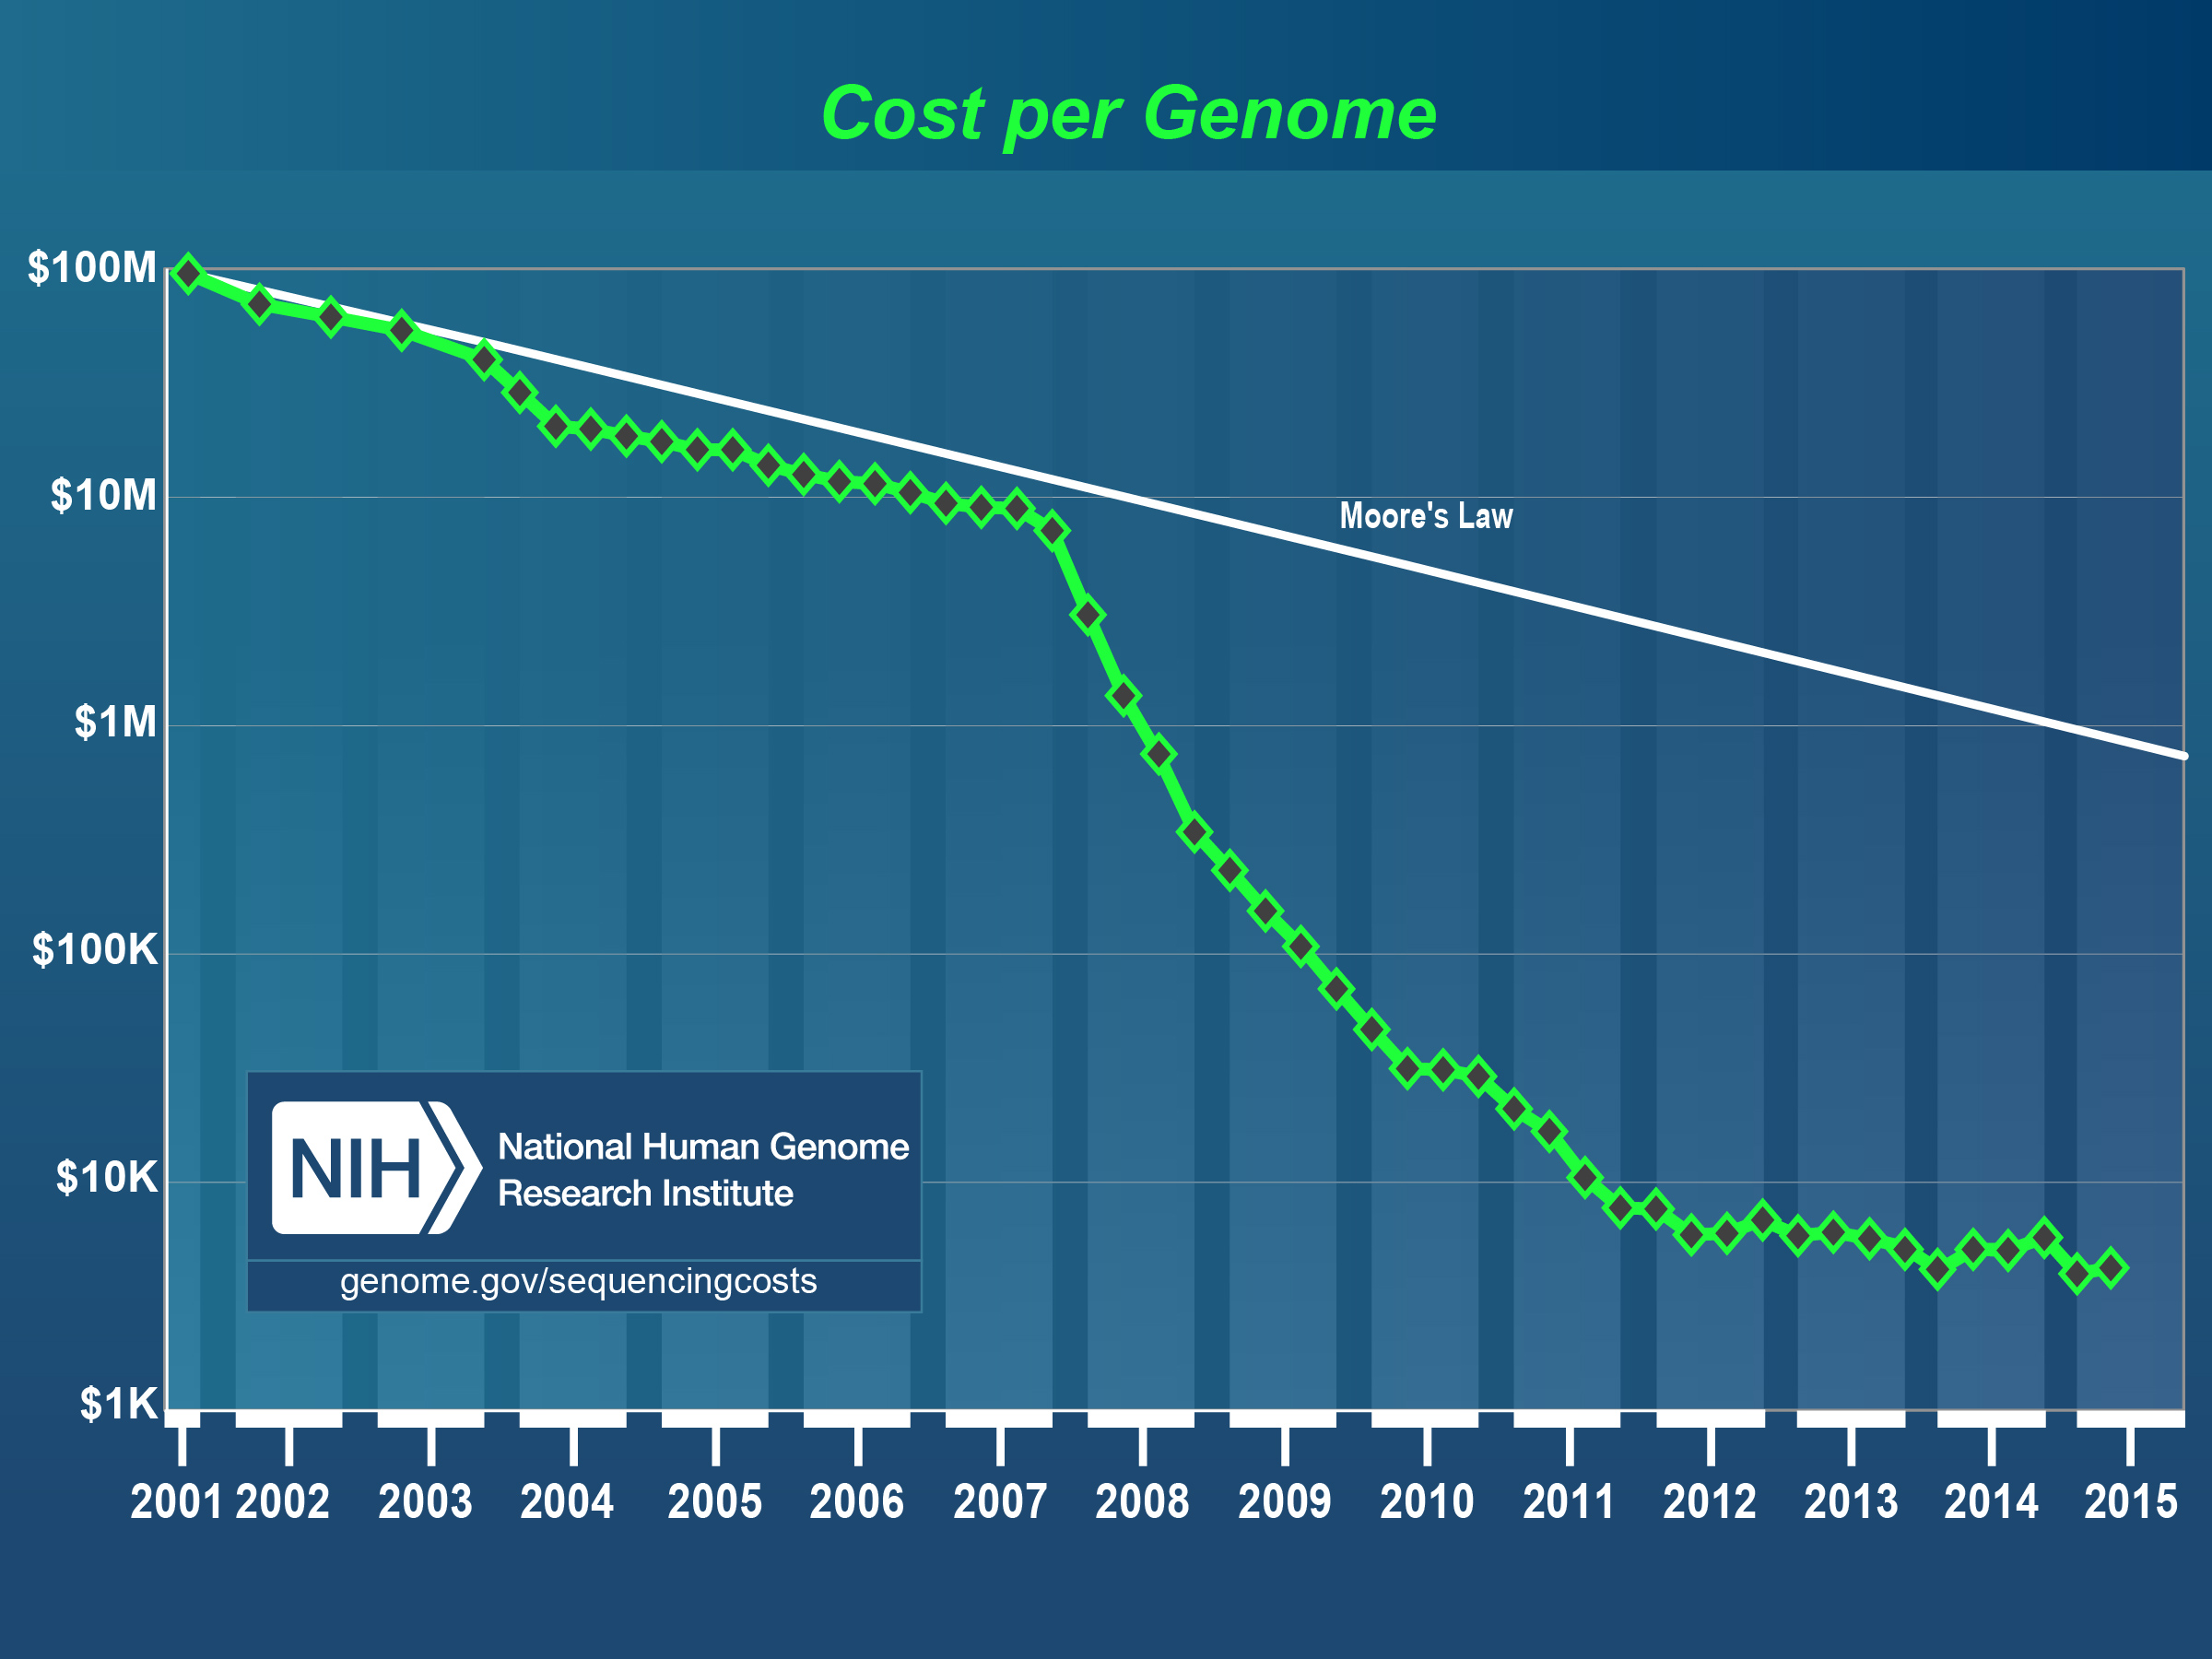
\includegraphics[width=0.7\textwidth]{cost_genome.jpg}
\end{center}





\cleardoublepage




\section{Contexte technologique}

\subsection{L'ADN et le séquençage}

Les bio-polymères, et notamment l'ADN (Acide DésoxyriboNucléique), sont les polymères qui constituent le vivant. Ils interviennent dans de nombreux processus clés en biologie.  L'ADN, avec l'ARN (Acide RiboNucléique) est le support de l'information génétique du vivant. \\

L'ADN, généralement contenu dans le noyau des cellules, a été pour la première fois isolé et identifié par Friedrich Miescher en 1869 à partir de globules blancs. En 1953, Francis Crick et James Watson mettent en évidence sa fameuse structure en double hélice \cite{watsoncrick}. Cette hélice est le reflet de la conformation dite double brin de l'ADN, il s'agit de l'appariement de deux chaînes dites simple brin qui sont complémentaires. Le simple brin d'ADN est une séquence de quatre monomères différents. Ces monomères, appelés nucléotides sont constitués de phosphate, de sucre et d'une des bases azotées, seul élément distinct entre nucléotides: l'adénine, la guanine (deux purines), ainsi que la cytosine et la thymine (deux pyridines). Via des liaisons hydrogènes (aussi appelée liaisons Watson-Crick dans le cas de l'ADN), les bases peuvent s'associer à leur complémentaire, adénine avec thymine et cytosine avec guanine. Les liaisons hydrogènes favorisent une forte affinité lors de l'appariement et contribuent avec les interactions orbitalaires entre cycles aromatiques des bases azotées à stabiliser cette structure hélicoïdale.

\begin{figure}[H]
\begin{center}
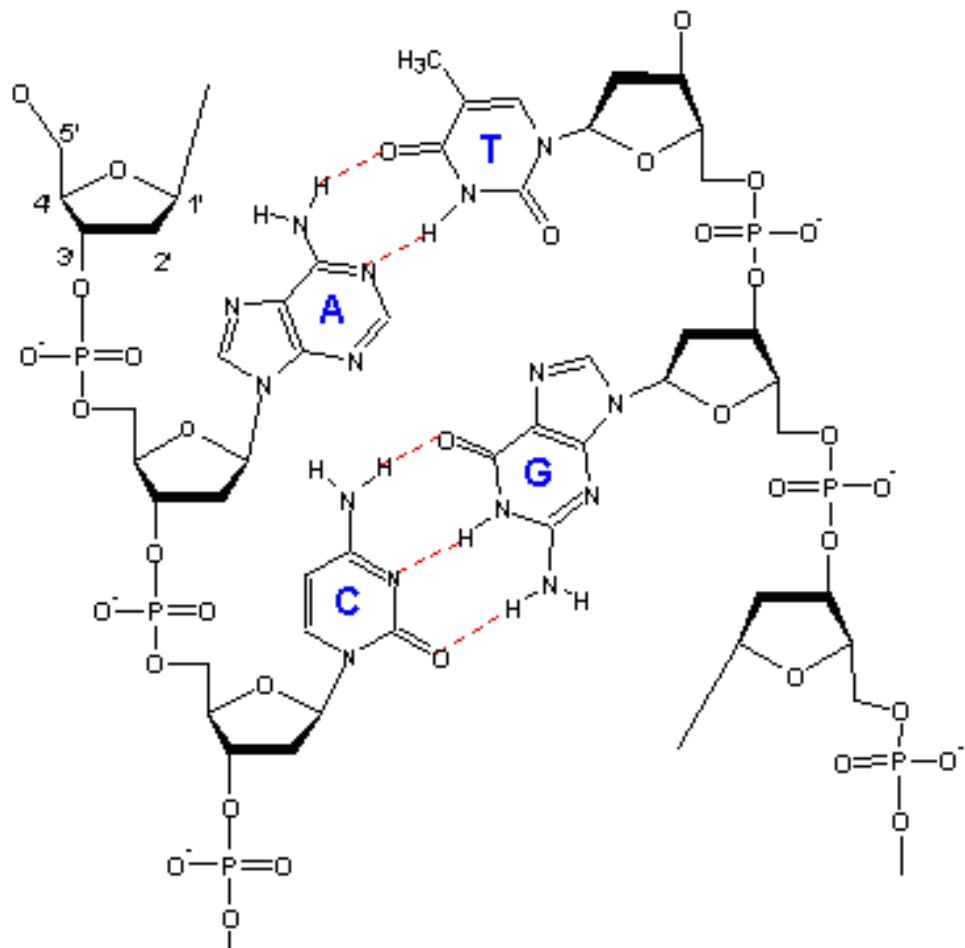
\includegraphics[width=0.63\textwidth]{adn.jpg}

\caption[Représentation de l'ADN]{Structure chimique de l'ADN. Le squelette est composé d'une succession de phosphates et de sucres liés entre eux. Chacun des sucres est de plus lié à une base azotée. Les bases azotées peuvent interagir par liaisons hydrogènes et interactions orbitalaires. Les bases s'associent plus facilement avec leur complémentaire (Adénine et Thymine ou Cytosine et Guanine) permettant une certaine variété de structure: repliement d'ADN simple brins ou encore association de deux cha\^{i}nes complémentaires formant l'hélice caractéristique de l'ADN dit double brins (image empruntée au cours de Sergei N. Smirnov \cite{adnjpg}).}
\label{adn}
\end{center}
\end{figure}

La structure chimique de l'ADN et ses interactions (rappelées sur la figure \ref{adn}) génèrent des propriétés qui sont fortement dépendantes de la séquence. L'influence de la séquence et la compréhension du vivant passe par la capacité à séquencer l'ADN, c'est à dire déterminer l'enchaînement des nucléotides. \\

Les applications sont potentiellement nombreuses: caractérisation d'espèces vivantes \cite{Sanggaard2014}, identification de souches pathogènes pour les virus ou bactéries \cite{Janda2007}, diagnostique des maladies génétiques \cite{Saunders2012}, étude de la phylogénie \cite{Neves2011}, analyse de la résistance aux antibiotiques  \cite{Davies2010}, identification de mutations \cite{Schneeberger2009}, médecine personnalisée \cite{Hamburg2010}, identification d'individu pour la police scientifique \cite{Wilson1995}.\\


Dès la deuxième moitié des années 70, les premières méthodes de séquençage voient le jours. Il s'agit de la méthode de Sanger \cite{Sanger1975} (voir figure \ref{sangermethod}) basée sur une synthèse enzymatique sélective (inspirée des travaux de Wu et al \cite{WU1972}, qui déterminèrent la première séquence de 24 paires de bases) et de la méthode Maxam et Gilbert \cite{Maxam1977} basée sur une dégradation chimique sélective. Gilbert et Sanger obtiennent tous les deux le prix Nobel de médecine en 1980 pour leurs méthodes. En 1977, grâce à sa méthode, Sanger parvient à séquencer le premier génome complet, il s'agit du bactériophage $\Phi$X174 \cite{Sanger1977}.\\

\begin{figure}[H]
\begin{center}
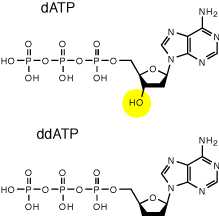
\includegraphics[width=0.5\textwidth]{ddatp.png}\hspace{1.3cm} 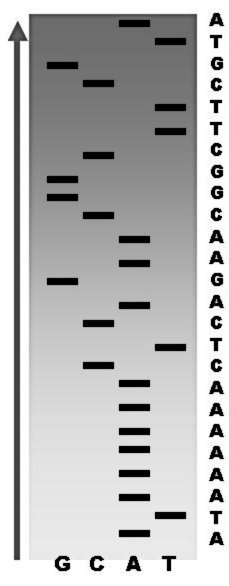
\includegraphics[width=0.21\textwidth]{gelelectrophoresis.jpg}
\vspace{0.5cm}

\caption[Séquencer par la méthode de Sanger]{Le séquençage par la méthode de Sanger : Le brin d'ADN à séquencer est répliqué parallèlement dans quatre milieux différents contenant chacun les quatre désoxyribonucléotides triphosphate (dATP, dCTP, dGTP, dTTP). Chacun des milieux présente en plus une faible quantité de l'un des didésoxynucléotides triphosphate (ddATP, ddCTP, ddGTP ou ddTTP), qui une fois incorporé dans la cha\^{i}ne empêche toute croissance supplémentaire (image de gauche). Chacun des quatre milieux présente alors des cha\^{i}nes de tailles variées terminant toutes par un même nucléotide. Les milieux sont alors analysés par électrophorèse sur gel, ce qui va trier les cha\^{i}nes par taille. On peut alors remonter à la séquence par lecture directe sur le gel (image de droite).}
\label{sangermethod}
\end{center}
\end{figure}



 
 La méthode de Sanger est rapidement préférée à celle de Maxam-Gilbert car elle nécessite moins de composés chimiques toxiques et de marqueurs radioactifs. Elle a été utilisée du début des années 80 jusqu'à la moitié des années 2000 avec principalement des avancées techniques:  marquage fluorescent \cite{Prober1987}, électrophorèse capillaire \cite{Swerdlow1991} ou encore automatisation des procédures \cite{Hunkapiller1991}.\\
 
  Afin de séquencer de longs génomes, les nouvelles techniques utilisent la méthode dite shotgun, élaborée par R. Staden \cite{Staden1979}, qui reconstruit un génome complet à partir de fragments de séquences moins coûteux et plus simples à séquencer (voir figure \ref{shotgun}).
 


\begin{figure}[H]
\begin{center}
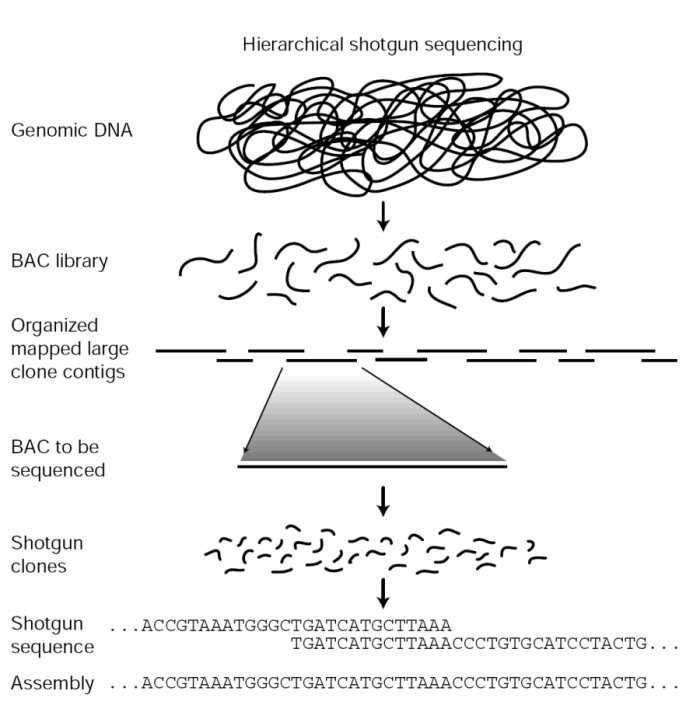
\includegraphics[width=0.75\textwidth]{shotgun.jpeg}
\vspace{0.5cm}

\caption[Méthode Shotgun]{Schéma de principe de la méthode shotgun (emprunt à l'article de revue de Eric S. Lander et al.\cite{Lander2001}). Le brin étudié est d'abord copié de nombreuses fois par PCR. Les brins sont ensuite fragmentés pour créer une banque de séquences aléatoires plus courtes (et moins compliquées à séquencer) qui sont également marquées. Ces fragments subissent à nouveau une PCR et forment de nombreux clones rassemblés chacun dans une colonie (ou polonie, contraction de PCR et colonie, voir figure \ref{pcr}). Chaque colonie est alors séquencée. De lourds traitements informatiques sont enfin employés pour reconstituer la séquence d'origine à partir des parties de génomes qui se chevauchent entre séquences.}
\label{shotgun}
\end{center}
\end{figure}

 En plus de nécessiter une librairie de base, ces techniques impliquent une amplification du signal ADN de départ par PCR (Polymerase Chain Reaction) \cite{Saiki1985}, de lourd traitements algorithmiques et sont sujettes à des erreurs notamment en ce qui concerne les parties de séquences redondantes dont certaines peuvent être omises. 


 \begin{figure}[H]
\begin{center}
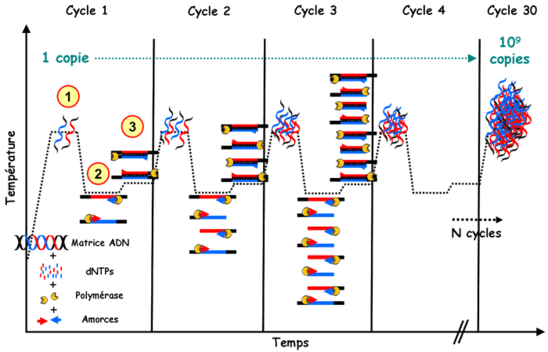
\includegraphics[width=0.85\textwidth]{pcr.png}

\vspace{0.5cm}

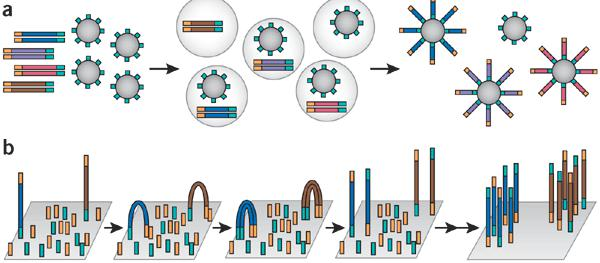
\includegraphics[width=0.85\textwidth]{bridgepcr.jpg}
\vspace{0.5cm}

\caption[PCR]{En haut, schéma de principe d'une PCR (Polymerase Chain Reaction), emprunt au site de l'université de Strasbourg \cite{pcrjpg}. Plusieurs cycles sont effectuées dans un milieu contenant la séquence à répliquer, des oligonucléotides amorces spécifiques, des polymérases et des nucléotides. La température est élevée jusqu'à 95°C pour dénaturé l'ADN et le rendre simple brin, elle est ensuite baissée entre 45 et 70°C pour que les amorces s'arriment aux brins de séquence à reproduire, et enfin la température est ré-élevée à 72°C pour réaliser la croissance des brins complémentaires par la polymérase. En bas, illustration de l'article de revue de Shendure \cite{Shendure2008}. a/ Une PCR réalisée en émulsion, les cycles successifs de température sont réalisés au sein d'une goûte en suspension. b/ Une PCR sur lame de microscope, la multiplication de l'ADN a lieu sur une zone restreinte grâce à un système de liaison covalentes avec les amorces de la réaction. Chaque goutte en suspension ou chaque zone sur la lame de microscope est appelée colonie d'ADN (ou polonie, contraction de PCR et colonie). Une polonie contient un unique fragment de la banque d'ADN. Les différents appareils commerciaux se distingueront dans un premier temps uniquement dans la façon d'effectuer la PCR et/ou de séquencer ces polonies.}
\label{pcr}
\end{center}
\end{figure}

Deux types de PCR seront successivement utilisées. La PCR en émulsion \cite{Williams2006}, puis la PCR directement sur lames de microscopes \cite{Shendure2005}. La figure \ref{pcr} présente le concept de PCR et ces deux exemples. Cette première génération de séquençage a permis en 2001 le premier séquençage complet du génome humain \cite{Lander2001,Venter2001}, Graal du Human Genome Project pour un coût total estimé de 3 milliards de dollars \cite{adncost}.


Brevetées dans les années 90 \cite{tsien1991dna,farinelli1998method}, les méthodes précédemment décrites vont être utilisées dans des appareils de séquençage commerciaux, ce qui va populariser l'utilisation du séquençage \cite{Schuster2007}. Ces appareils se distinguent principalement par les moyens utilisés afin de séquencer la banque d'ADN obtenue dans le cadre de la méthode shotgun. Le premier appareil de cette génération, le MPSS (Massively parallel signature sequencing \cite{Brenner2000}) voit le jour en 2000. Il repose sur une méthode tellement complexe qu'aucun appareil n'a été fourni à des laboratoires indépendants, les séquençages ayant lieux dans les locaux de la compagnie Lynx Therapeutics.

 D'autres appareils sont développés en parallèle. En 1996 le pyrosequencing \cite{Ronaghi1996}, séquençage qui repose sur la détection de l'activité de l'ADN polymérase par un pyrophosphate voit le jour. Ce procédé sera utilisé par un appareil commercial de la société 454 Life Sciences en 2005 \cite{Margulies2005}. Life Technologies avec le séquençage SOLiD \cite{mckernan2007reagents,Cloonan2008} (Sequencing by Oligonucleotide Ligation and Detection) commercialise son appareil en 2008. Il s'agit de séquençage par ligation, ce dernier repose sur une identification de la séquence par la forte spécificité de l'ADN ligase, qui va lier à l'aide d'une séquence de référence, un brin complémentaire, préalablement marqué, à la séquence inconnue. La partie liée est caractéristique de deux bases successives. 
% Quatre flurophores différents sont utilisés et chacun des fluorophores est donc caractéristique de quatre doublets de bases ( il y en a $2^{4}=16$ différents répartis sur quatre fluorophores).
 Des lectures successives en décalant les ligations d'une base permettent de déduire la séquence. Ce système a vu le jour dans un premier temps avec une PCR en émulsion puis une version utilisant une PCR sur support solide a été développée. Cette technique est efficace mais présente cependant des erreurs lors de la lecture de séquences formant des palindromes \cite{Huang2012}.
 
  La société Illumina en 2008 \cite{Bentley2008} sort le premier appareil basé sur une PCR sur support solide. Le séquençage est réalisé par la lecture de fluorophores lors de l’incorporation de bases modifiées au cours de la PCR. Le marquage est retiré à chaque étape de lecture. Life Technologies utilise quant à elle aussi le séquençage par semi conducteurs pour détecter les ions hydrogènes relâchés lors de la polymérisation de l'ADN (Ion semiconductor sequencing) \cite{Rusk2010}. Cette méthode est efficace, mais rencontre des  problèmes avec les répétitions d'homopolymères \cite{Rusk2010}. 

\begin{figure}[H]
\begin{center}
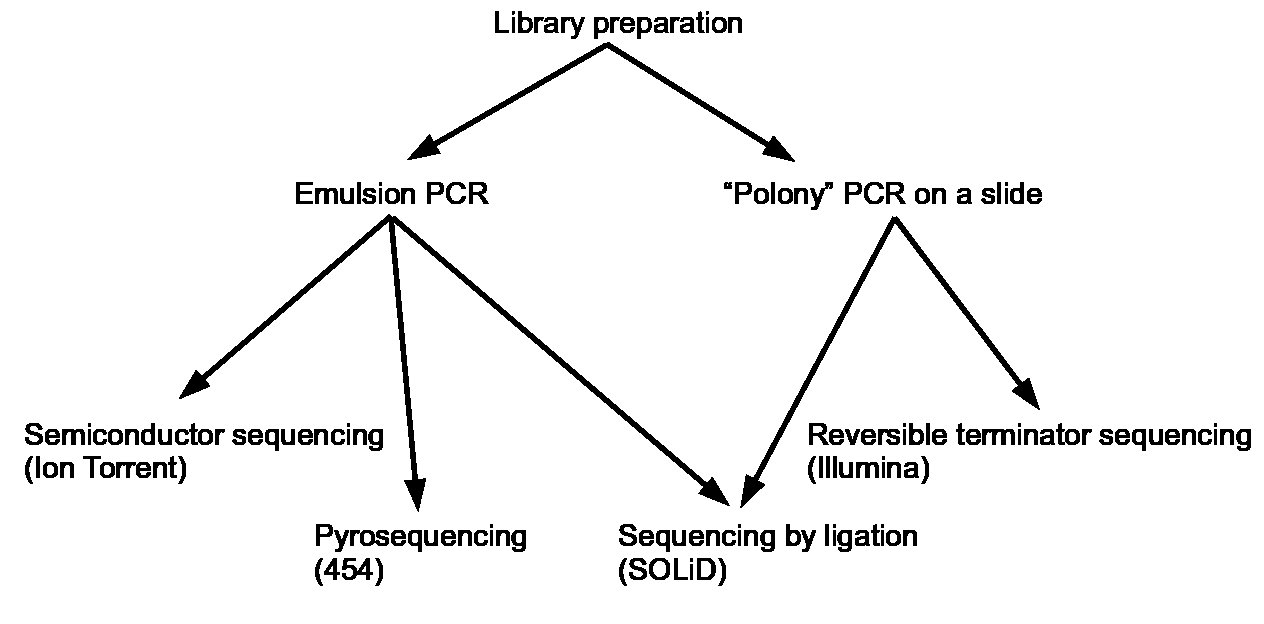
\includegraphics[width=0.8\textwidth]{ngsprinciple.jpg}
\vspace{0.5cm}

\caption[Principe du séquençage nouvelle génération]{Schéma récapitulatif du fonctionnement des premiers appareils de séquençage de nouvelle génération \cite{ngsprinciplejpg}.}
\label{ngsprinciple}
\end{center}
\end{figure}

Comme nous l'avons vu, ces procédés nécessitent une PCR pour amplifier le signal ADN de départ. Cette étape est source d'erreurs, en effet la PCR peut être biaisée et peut générer des artefacts \cite{Acinas2005}.



Deux autres techniques de lecture sans amplification sont développées, DNA nanoball sequencing \cite{Porreca2010} et Heliscope single molecule sequencing \cite{pmid20890904}, mais restent peu utilisées car elles ne sont utilisables que sur des fragments d'ADN très courts. Une approche originale est également commercialisée, il s'agit du séquençage en temps réel d'une molécule unique (Single molecule real time sequencing), un marquage fluorescent est détecté lors de la création du brin complémentaire lors de la copie de l'ADN \cite{Eid2009}. Cependant plusieurs lectures sont nécessaire pour obtenir une précision suffisante \cite{Chin2013}. Ces derniers appareils sont précurseurs de la troisième génération de séquençage en manipulant des molécules uniques.



Certains de ces appareils sont comparés dans les articles de revue de Quail et al. \cite{Quail2012} et de Liu et al. \cite{Liu2012}. 

\begin{figure}[H]
\begin{center}
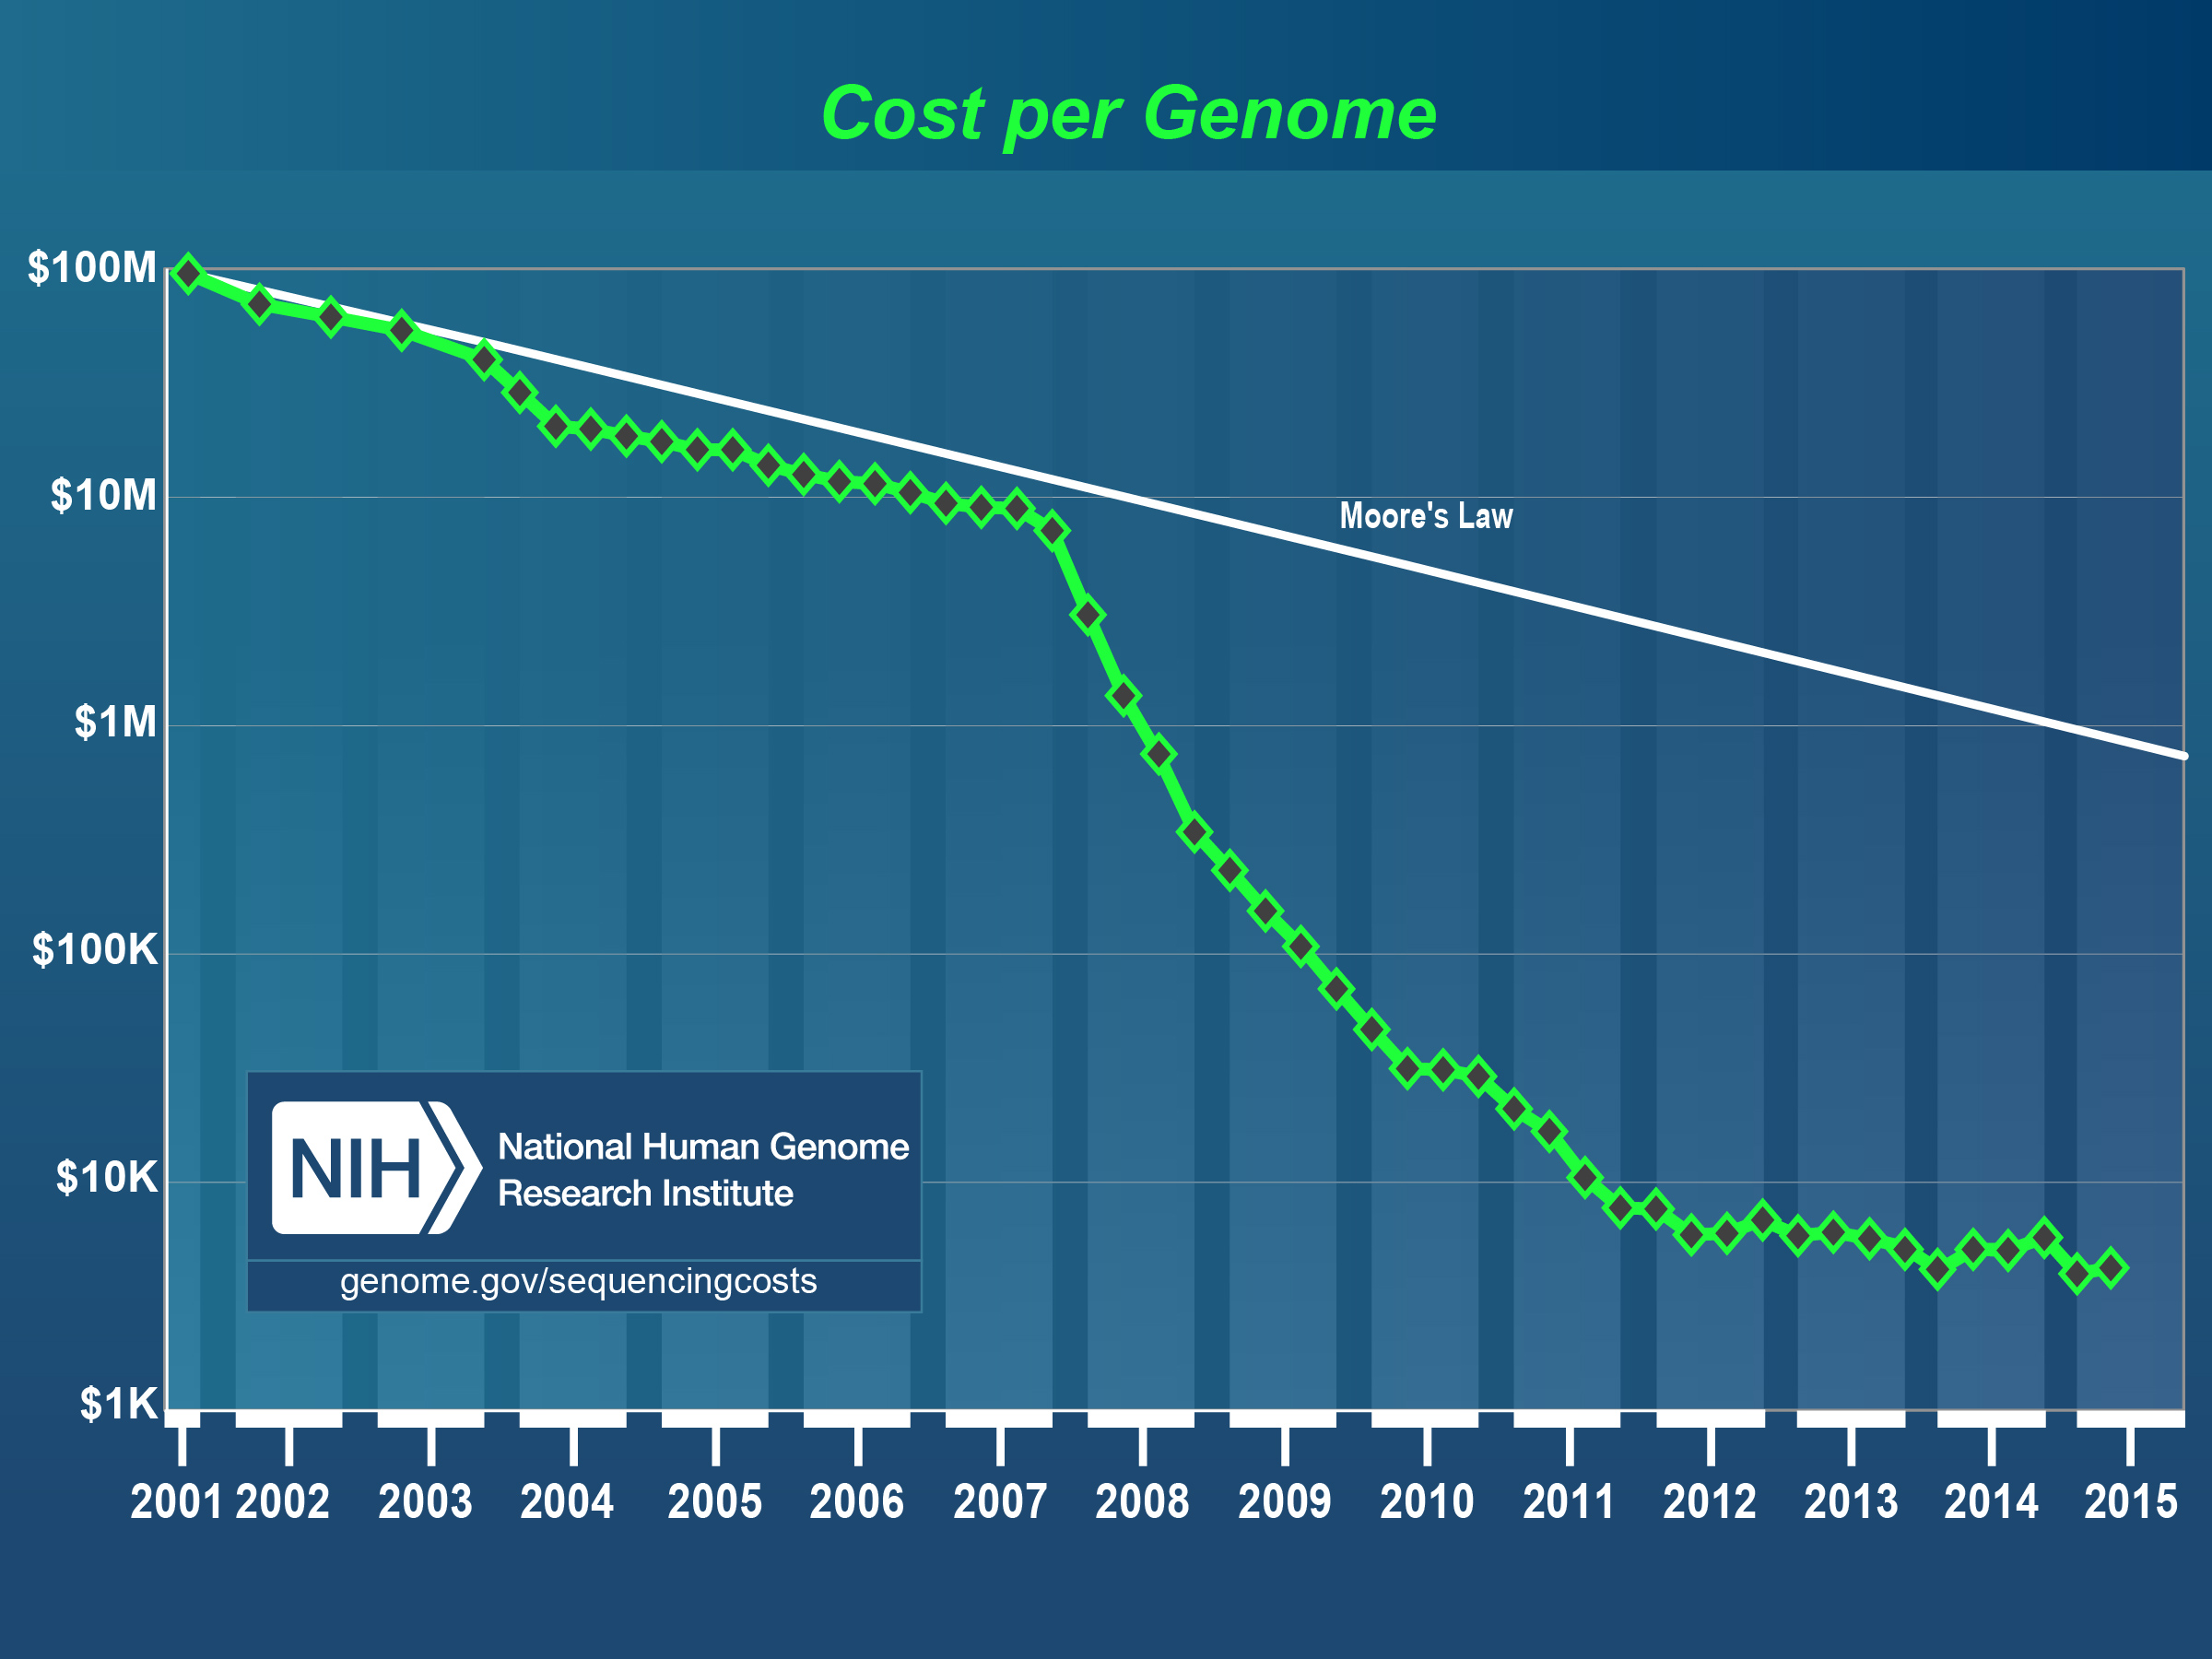
\includegraphics[width=0.7\textwidth]{cost_genome.jpg}

\caption[Coût du séquençage]{Evolution du coût du séquençage d'un génome complet selon le NIH \cite{adncost}. On observe au départ une diminution normale du coût suivant une loi de Moore. L'arrivée des premiers appareils commerciaux de séquençage de nouvelle génération se traduit par une rupture de pente très nette en 2007. Aujourd'hui, un plateau au dessus de l'objectif des 1000 USD pour un génome complet est atteint, d'où la nécessité de développer des méthodes dites de troisième génération.}
\label{seqcost}
\end{center}
\end{figure}


Tous ces appareils commerciaux  ont fait leurs preuves mais leur utilisation demeure trop coûteuse pour envisager leur usage à grande échelle. Une troisième génération de technique de séquençage est aujourd'hui envisagée. La figure \ref{seqcost} présente l'évolution du coût du séquençage d'un génome complet. Nous sommes toujours au dessus de l'objectif de 1000 USD \cite{Mardis2006}.
\\

Voici une liste de pistes envisagées pour les appareils de séquençage de troisième génération:

\begin{itemize}


\item Le séquençage par hybridation \cite{Zhang2003}. Ce procédé permet de reconnaître des séquences types par leur hybridation avec des bio-puces à ADN (de courtes séquences), cela nécessite un marquage fluorescent ainsi qu'un nombre important de produits chimiques et d'ADN de base.

\item L'utilisation de la spectroscopie de masse \cite{Edwards2005}. Basée sur la différence de masse entre les nucléotides, cette méthode semble être adaptée à la détection de substitution de bases dans différents gênes, mais pas pour séquencer des génomes de novo (dans leur intégralité). Elle s'avère utile cependant pour la médecine légale \cite{Howard2013}. 

\item La mise au point de techniques de microscopie électronique \cite{Bell2012}. Ces techniques sont complexes car elles nécessitent une modification des bases de l'ADN pour incorporer des atomes au numéro atomique élevé, afin d'obtenir un contraste suffisant.

\item La manipulation de bio-molécules avec pinces optiques, magnétiques ou AFM \cite{Pareek2011,Ding2012}.

\item La mesure du courant obtenu par effet tunnel lors du passage de l'ADN dans un canal microfluidique \cite{Ohshiro2012,DiVentra2013}.

\item \textbf{Le séquençage par nanopore.}


\end{itemize}


C'est cette dernière possibilité que nous explorons !

\subsection{Utilisation de nanopores et types de pores}

Le séquençage par nanopore a potentiellement de nombreux avantages sur les systèmes commerciaux déjà existants. En effet, cette technique laisse envisager la lecture de longues séquences (supérieurs à 5000 paires de bases) à vitesse élevée (1 paire de base par nanoseconde) \cite{Timp2010,Branton2008}. Aucun marquage chimique n'est nécessaire, l'utilisation d'enzymes est moindre et le signal ADN n'a pas besoin d'être amplifié (pas de PCR).

Exposons dans un premier temps les concepts de bases et définitions du séquençage par nanopore. On envisage de séquencer la séquence ADN au cours de sa translocation. Il s'agit du passage d'un polymère d'un coté, appelé cis, d'une membrane à l'autre, appelé trans, à travers un pore (voir figure \ref{translocbase}). Cette translocation peut être naturelle (non biaisée) ou pilotée par une force (biaisée). La translocation est un phénomène biologique fréquent, c'est le cas par exemple lorsqu'un virus infecte une cellule en y translocant son ADN.

\begin{figure}[H]
\begin{center}
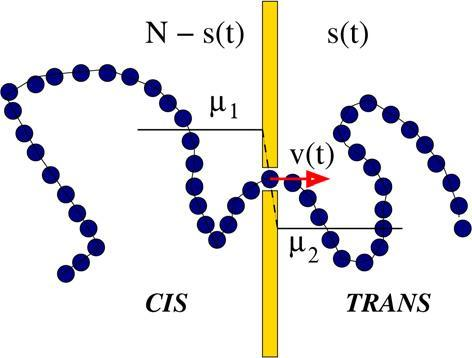
\includegraphics[width=0.44\textwidth]{translocation.jpg} 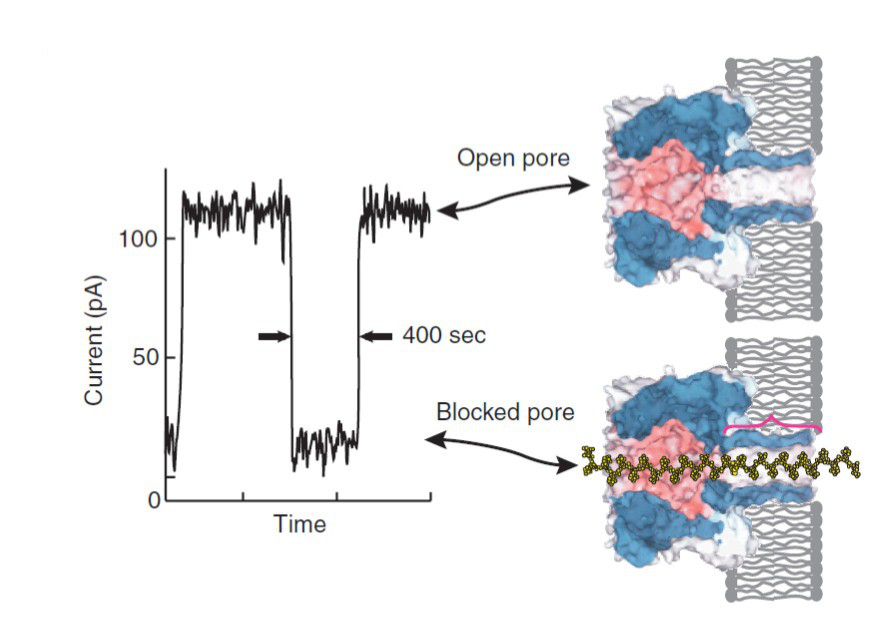
\includegraphics[width=0.55\textwidth]{translocissues.jpg}

\caption[Translocation et courant de blocage]{Translocation d'un polymère. A gauche: Illustration de la translocation biaisée d'un polymère par l'application d'une différence de potentiel chimique empruntée à l'article de revue de A. Milchev \cite{Milchev2011}. A droite: Translocation d'ADN à travers un bio-pore et mesure du courant de translocation illustrés par Branton et al. \cite{Branton2008}.}
\label{translocbase}
\end{center}
\end{figure}

Au cours de la translocation de l'ADN, on espère pouvoir séquencer en mesurant le courant de translocation. Le principe est simple, au cours de la translocation, l'occupation du pore entraîne une modification de sa résistance électrique, modification caractéristique de l'entité occupant ce pore. On peut alors espérer déterminer la nature de l'occupant du pore (typiquement la séquence pour l'ADN) en mesurant le courant ionique de blocage du pore (voir figure \ref{translocbase}). On dispose déjà de certaines applications de ce procédé, notamment pour le comptage de polymères \cite{Bezrukov1994}, la détection d'ADN et ARN \cite{Kasianowicz1996} ou encore la discrimination de certains polynucléotides \cite{Akeson1999,Meller2000,Ashkenasy2005}. Cette technique bien que prometteuse admet des limites de résolution spatiales et temporelles qui font qu'elle ne permettra pas de séquencer l'ADN \cite{Branton2008}. Nous expliquerons ces limites en décrivant les différent types de nanopores disponibles ainsi que les techniques alternatives qui s'inspirent de la mesure du courant ionique de blocage, dans le paragraphe suivant.

%\textcolor{red}{c'est démontré que courant ionique classique ne peut pas distinguer donc courant transverse ou fonctionnalisation. j en parlerais après description des différents nanopores.}

\subsubsection{Les biopores}


Historiquement, les premier nanopores utilisés sont ceux fournis par la nature. On peut employer la protéine F située sur la membrane extérieure de Escherichia Coli \cite{Danelon2006,Chimerel2008}) ou encore l'$\alpha$-hémolysine du Staphylocoque doré \cite{Bhakdi01121991}. Ce dernier est très utilisé car il est disponible commercialement, d'une reproductibilité parfaite et susceptible d'être employé avec de l'ingénierie génétique pour modifier certaines propriétés (blocage au passage d'ADN par exemple \cite{Howorka2001}). Il s'agit d'ailleurs du bio-pore utilisé par Kasianowicz et al. pour effectuer en 1995 la première translocation d'ADN \cite{Kasianowicz1996}.


\begin{figure}[H]
\begin{center}
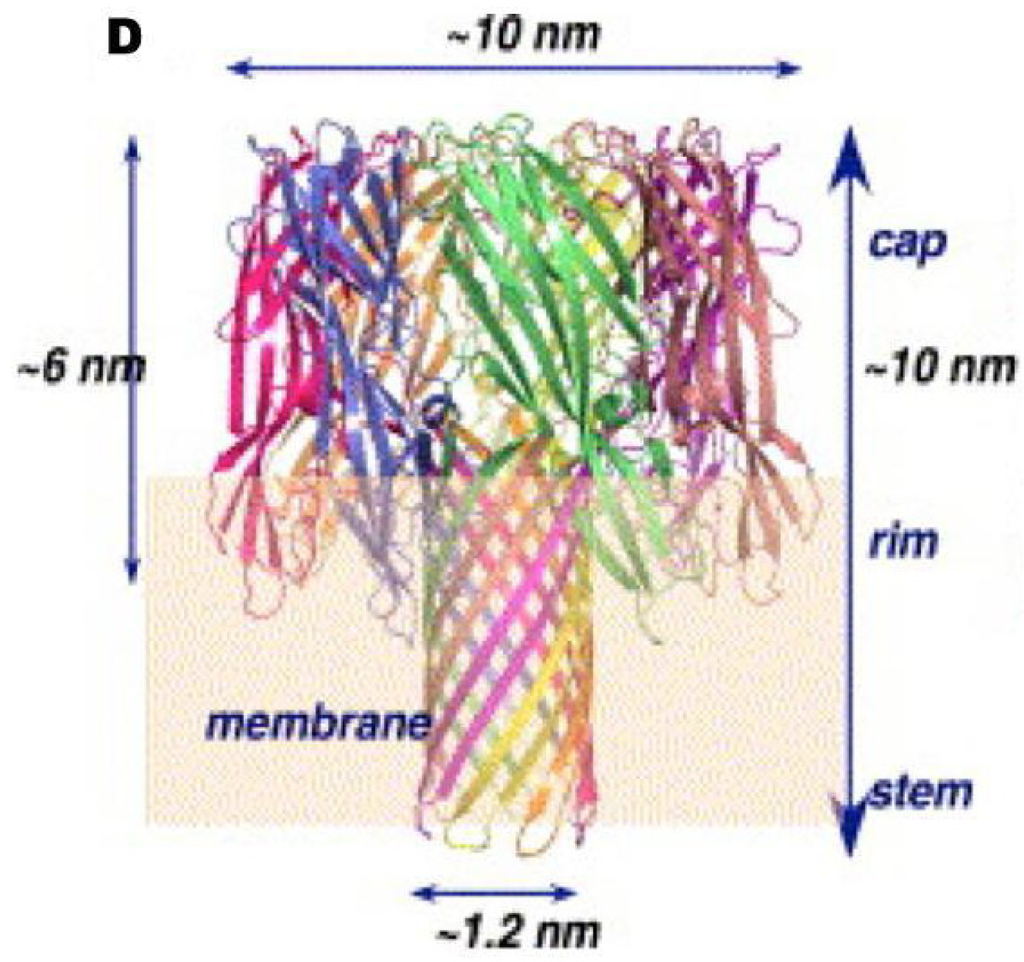
\includegraphics[width=0.51\textwidth]{bioporetoxine.png}
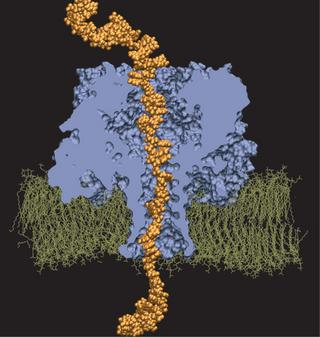
\includegraphics[width=0.42\textwidth]{biopore2.jpg}

\caption[Biopores]{Les bio-pores ont été les premiers pores utilisés à des fins d'étude ou d'emploi des phénomènes de translocation. A gauche, modèle du pore heptameric de B. cereus \cite{Ramarao2013}. A droite, simulation de translocation d'ADN à travers un bio-pore ($\alpha$-hémolysine) \cite{Aksimentiev2010}.}
\label{biopore}
\end{center}
\end{figure}


Ces bio-pores ont prouvé leur efficacité pour la translocation d'ADN et ARN simples brins ou encore pour des protéines dépliées \cite{Movileanu2005}. Ils demeurent trop étroit pour les formats double brins car leur diamètre n'est pas réglable. La nature fournie des outils efficaces, car avec l'utilisation en complément de protéines chaperonnes, il est possible d’empêcher l'inversion de la translocation \cite{DeLosRios2006} (phénomène qui inspira la fonctionalisation des autres types de pores dont nous allons parler par la suite). La figure \ref{bioporepossib} présente un inventaire succins des possibilitées offertes par les bio-pores. 
\begin{figure}[H]
\begin{center}
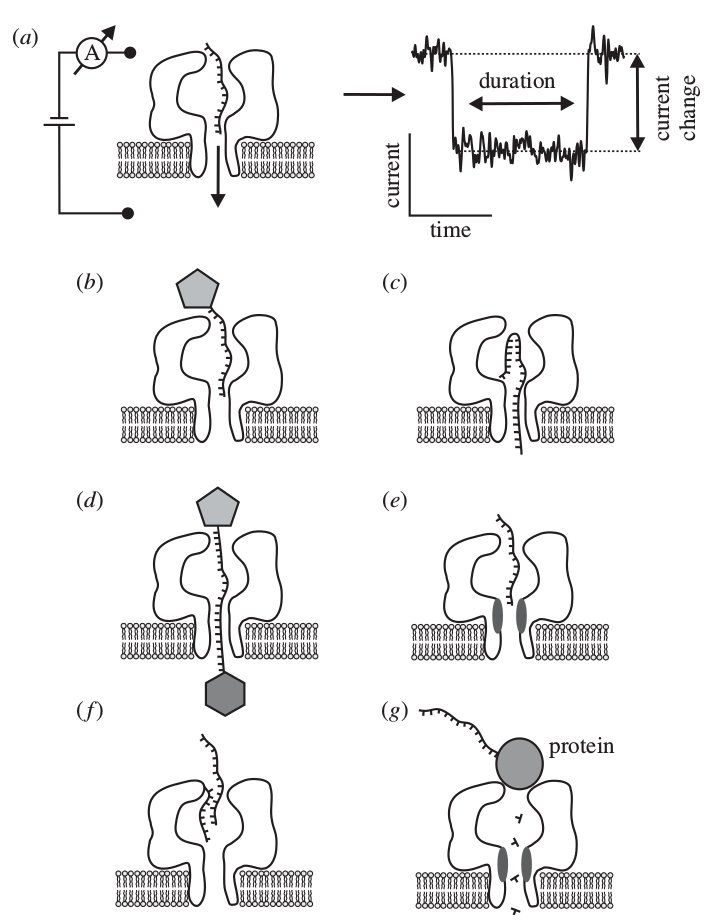
\includegraphics[width=0.85\textwidth]{bionanopore.jpg}


\caption[Manipulations sur bio-pores]{Différentes manipulation possibles avec les bio-pores (emprunt à l'article de revue de U. F. Keyser \cite{keyser}). a/ Mesure du courant ionique de translocation. b/ Une protéine plus large que le pore fixée sur l'ADN permet d'imposer le sens de la translocation. c/ Un brin replié sur lui même peut stopper la translocation. d/ Attacher une protéine à chaque extrémité de l'ADN peut conduire à une translocation à durée infinie. e/ La modification génétique du pore peut affecter la translocation. f/ Le pore peut être fonctionnalisé avec de l'ADN complémentaire d'une séquence à détecter. g/ Une endonucléase peut être combinée au nanopore pour réaliser une translocation base par base.}
\label{bioporepossib}
\end{center}
\end{figure}

Pour effectuer une translocation forcée à travers des bio-pores, l'outil principal demeure l'électrophorèse (potentiel électrique) \cite{Kasianowicz1996,Henrickson2000}. 
Dans une optique de séquençage, ils sont trop épais pour permettre de discriminer les séquences en cours de translocation car au sein du pore, se situent simultanément plusieurs dizaines de bases.

 L'utilisation d'une endonucléase (suggérée sur la figure \ref{bioporepossib}) par la société Oxford Nanopore Technologies est une possibilité pour surmonter ce problème. Un appareil commercial a vu le jour au cours de la thèse \cite{Mikheyev2014} et commence à être testé et utilisé \cite{Goodwin2015,Jain2015,Urban2015}. Leur technologie est décliné en plusieurs appareils allant du système portable au système de gros débit en format plus imposant \cite{oxfordnanopore} (voir figure \ref{oxfordnanopore}). 


\begin{figure}[h!]
\begin{center}

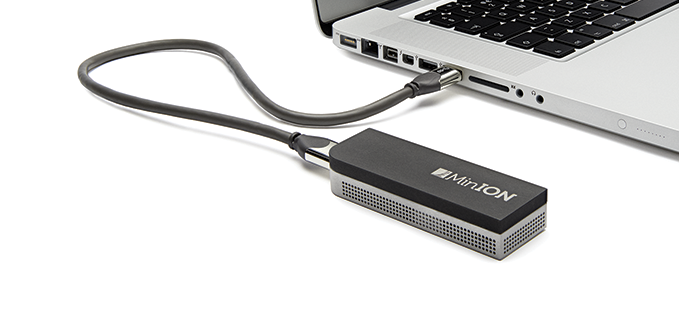
\includegraphics[width=0.5\textwidth]{MinION-Nanopore-technologies.png}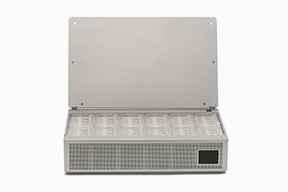
\includegraphics[width=0.5\textwidth]{PromethION-setup.jpg}

\caption[Séquenceur MinION]{Les appareils de séquençage, MinION et PromethION
de la société Oxford Nanopore Technologies \cite{oxfordnanopore}.}
\label{oxfordnanopore}

\end{center}
\end{figure}

Ces systèmes prometteurs présentent toujours des erreurs de lectures. Ces erreurs sont problématiques car la méthode est destructive pour l'échantillon. Afin de les contrôler il faudrait envisager une amplification du signal ADN de départ et donc l’utilisation de PCR et les mêmes inconvénients que nous avons vu précédemment. L'utilisation de bio-pores à des fins de séquençage est possible mais présente des contraintes auxquelles la communauté scientifique a rechercher un palliatif en développant des nanopores artificiels.



\subsubsection{Les premiers pores artificiels}


Les limites des bio-pores ont poussé les chercheurs à développer leur propres pores. En 2001 le premier nanopore artificiel est créé \cite{Li2001}. Un faisceau concentré d'ions ou d'électrons peut être utilisé pour creuser un pore dans une membrane de matériaux variés \cite{Wanunu2010}. Le silicium a été très utilisé. La figure \ref{artpore} illustre un pore typique vu par AFM.




\begin{figure}[h!]
\begin{center}
\begin{minipage}{0.45\linewidth}
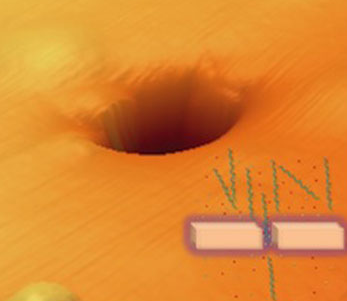
\includegraphics[width=\textwidth]{artificialpore.png}
\end{minipage}
\begin{minipage}{0.48\linewidth} 
\caption[Pores artificiels]{Vue par AFM d'un pore artificiel en silicium. Projet de l'université du texas \cite{artpore}. Bien que toujours épais, les nanopores de silicium présentent l'avantage d'être rigides, stables et de diamètres ajustables.}
\label{artpore}
\end{minipage}
\end{center}
\end{figure}

L'arrivée des nanopores artificiels a permis de travailler dans des conditions contrôlées. La possibilité de choisir le diamètre et les propriétés du pore s'accompagne du développement de techniques de manipulation pour forcer la translocation (voir la Figure \ref{solidstateporepossib}). L'électrophorèse est toujours possible \cite{Storm2005,2Storm2005,Wanunu2008}, cependant l'introduction des pores artificiels à également permis l'essort de l'utilisation de pinces magnétiques \cite{Peng2009} ou optiques \cite{Sischka2010}. Le ralentissement de la translocation en diminuant le diamètre du pore est également une possibilité \cite{Mirsaidov2010}. Afin de retrouver certaines propriétés des bio-pores, les pores artificiels peuvent aussi être fonctionalisés \cite{Mussi2010}. Certains ont même réalisé un couplage entre bio-pores et pore artificiels, en greffant une $\alpha$-hémolysine dans un nanopore de silicium \cite{Hall2010}, créant ainsi un pore hybride. La figure \ref{solidstateporepossib} montre les possibilités offertes par ces nanopore artificiels de première génération.


\begin{figure}[h!]
\begin{center}
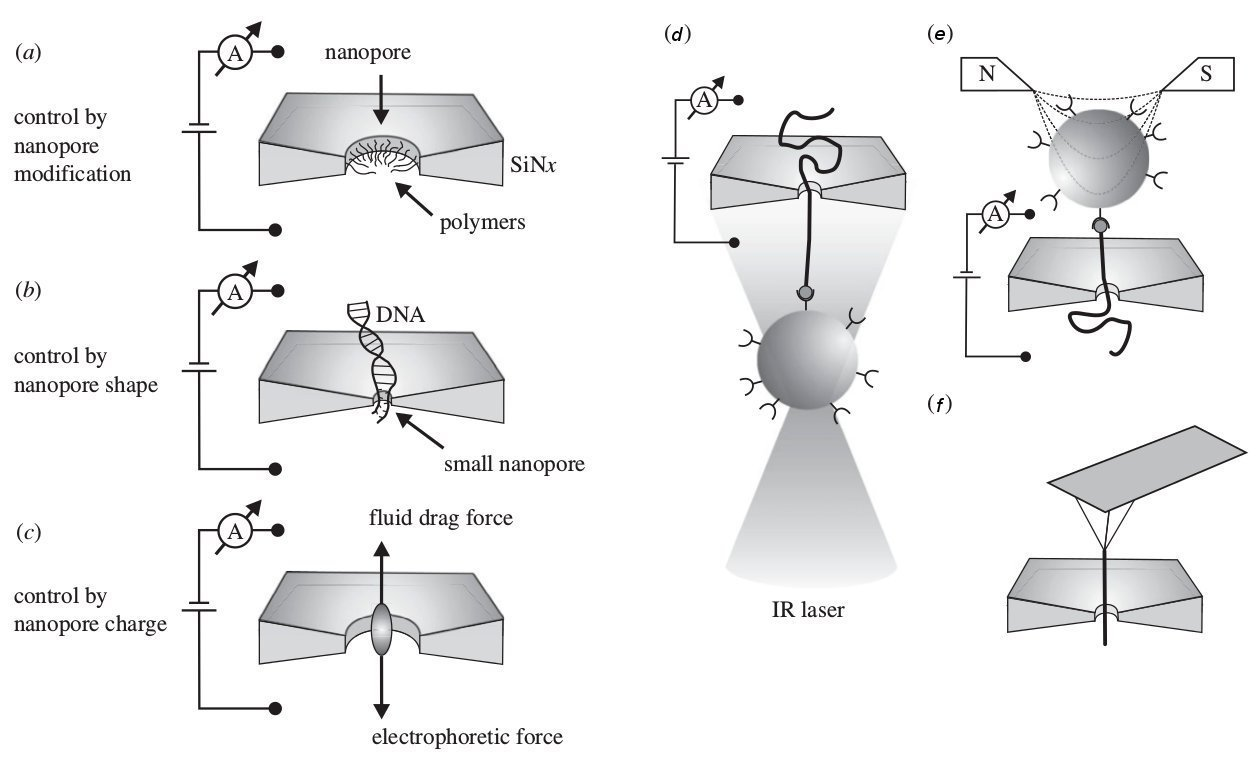
\includegraphics[width=1.0\textwidth]{solidstatenanopore.jpg}


\caption[Pores artificiels et manipulations]{A gauche, différentes modifications possibles avec les pores artificiels, à droite, les différents contrôles mécaniques possibles pour la translocation (emprunt à l'article de revue de U. F. Keyser \cite{keyser}). a/ Fonctionalisation du nanopore. b/ Gestion de la taille du nanopore. c/ Contrôle de la charge du pore (pouvant ralentir la translocation en générant une résistance hydrodynamique plus importante). d/ Utilisation de pinces optiques. e/ Utilisation de pinces magnétiques. f/ ADN accroché à une pointe d'AFM.}
\label{solidstateporepossib}
\end{center}
\end{figure}



Cette première génération de nanopores artificiels a permis d'effectuer des études quantitatives en variant certain paramètres, mais elle ne permet pas de relever le défi du séquençage non destructif. En effet l'épaisseur de ces dernier reste trop importante pour permettre la discrimination des séquences au cours de la translocation. Ceci fût un frein, jusqu'à l'isolation du graphène en 2004 par Andre Geim et Konstantin Novoselov \cite{Novoselov2004}. Ces derniers reçurent le prix Nobel de physique en 2010 pour leurs travaux sur le graphène.

\newpage

\subsubsection{Les pores artificiels fins}

L'arrivée du graphène marque le début d'une ère des possibles dans le domaine du séquençage par nanopores. En effet, le graphène étant un cristal bidimensionnel d'épaisseur mono-atomique stable, les problèmes de discrimination de la séquence au sein du pore sont potentiellement résolue par l'utilisation de membranes ultra fines. En 2010, Schneider et al. présentent la preuve expérimentale de la possibilité d'effectuer une translocation d'ADN à travers un nanopore dans une membrane de graphène\cite{Schneider2010}. L'utilisation du graphène présente de nouveau défis expérimentaux et théoriques car il présente, comme l'illustre la figure \ref{membvibgra}, des propriété vibrationnelles et est déformable.

\begin{figure}[h!]
\begin{center}
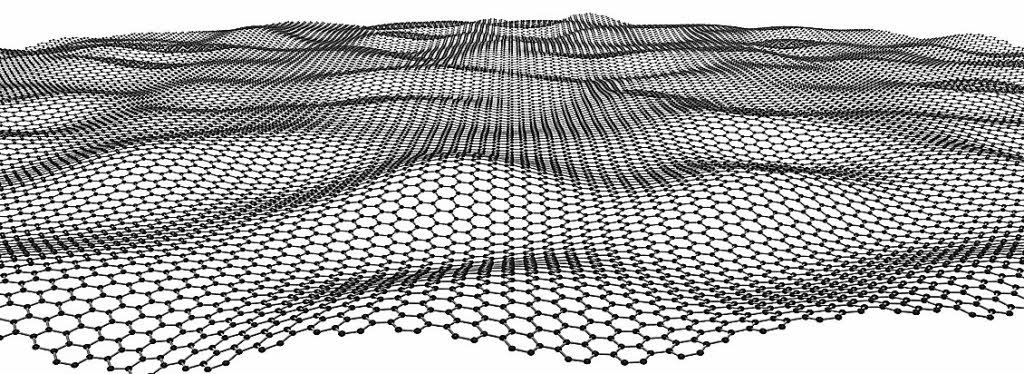
\includegraphics[width=0.84\textwidth]{vib.jpg}


\caption[Vibration et déformation d'une mono-couche de graphène]{Illustration de Jannik C. Meyer, qui a travaillé sur les membranes de graphènes \cite{Meyer2007}. La faible épaisseur des membranes monoatomiques entraîne une forte influence des vibrations, déformations et de la flexibilité.}
\label{membvibgra}
\end{center}
\end{figure}


Un autre cristal bidimensionnel est également envisagé, il s'agit du disulfure de molybdène \cite{Kang2014}, dans lequel des nanopores peuvent être creusés \cite{Feng2015} et une translocation effectuée \cite{2Feng2015}.

\begin{figure}[h!]
\begin{center}
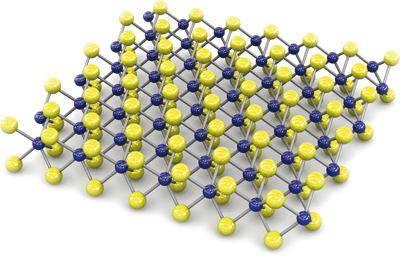
\includegraphics[width=0.78\textwidth]{MoS2.jpg}


\caption[Disulfure de molybdène]{Illustration de la structure du disulfure de molybdène \cite{Benameur2011}. Plus épais que le graphène, ce cristal bidimensionnel peut également être utilisé pour la translocation de polymères.}
\label{membvibmos2}
\end{center}
\end{figure}

Pour ces deux systèmes, il est possible d'effectuer une translocation mais sans pour autant pouvoir déterminer la séquence avec suffisamment de précision \cite{Schneider2010,2Feng2015}. Il est même possible d'envisager de créer des structures hybrides entre ces deux cristaux \cite{Roy2013}. Ces systèmes ont donc été modélisés pour voir comment améliorer la discrimonation des séquences (voir exemples de modèles sur la figure \ref{simultranslocboth}).

\begin{figure}[h!]
\begin{center}
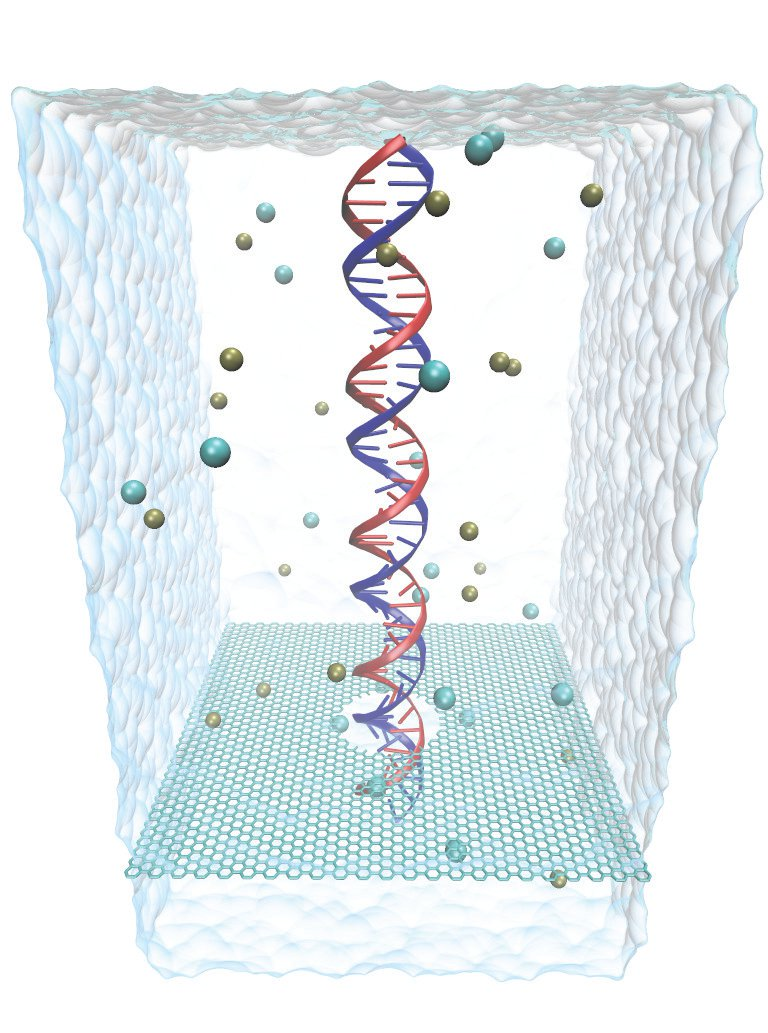
\includegraphics[width=0.45\textwidth]{dnatranslocsim.jpg}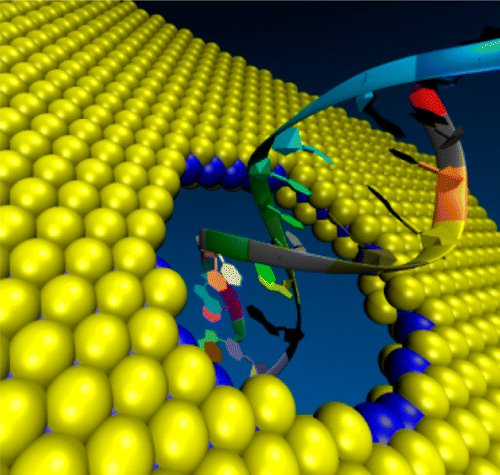
\includegraphics[width=0.55\textwidth]{mos2simul.jpg}

\caption[Translocation et cristaux bidimensionnels]{Simulations de la translocation d'ADN double brin à travers un nanopore dans des membranes de graphène \cite{Sathe2011} et de disulfure de molybdène \cite{Farimani2014}.}
\label{simultranslocboth}
\end{center}
\end{figure}

\newpage

\subsubsection{Les bio-pores fins}

En se basant sur la théorie développée par Seeman \cite{Seeman1982}, Rothemund a montré qu'il était possible de créer des Structures 2D d'ADN par autoassemblage \cite{Rothemund2006}. Le nom d'origami d'ADN a été donné à ses structures (pouvant également être développée à 3 dimensions \cite{Kuzuya2009}). Des exemples de structures 2D et 3D d'origami ADN sont présentés sur la figure \ref{origami}. 

\begin{figure}[H]
\begin{center}
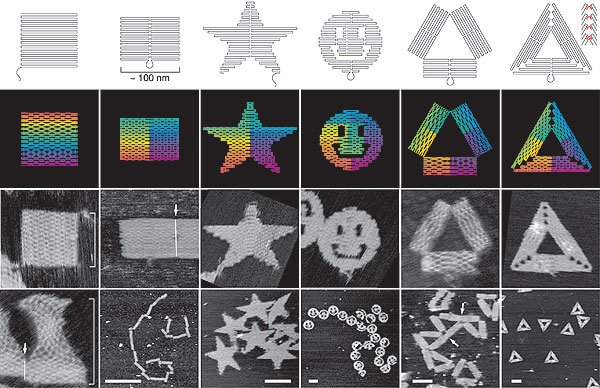
\includegraphics[width=0.8\textwidth]{origami2d.jpg}
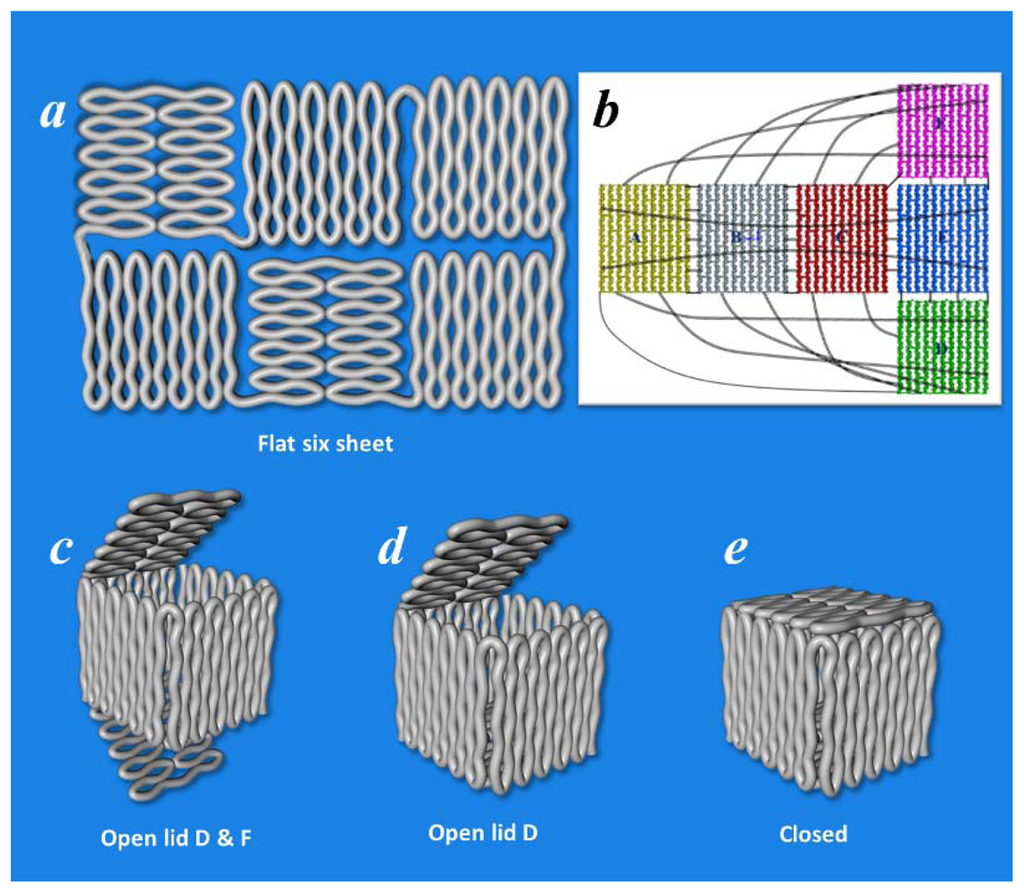
\includegraphics[width=0.8\textwidth]{origamis3d.png}

\caption[Origamis d'ADN]{Exemples de structures d'origamis ADN à 2\cite{Rothemund2006} et 3 dimensions \cite{Zadegan2012}.}
\label{origami}
\end{center}
\end{figure}

Ces structures d'ADN peuvent être utilisées afin de réaliser une membrane muni d'un nanopore \cite{2Bell2012}, au travers duquel il est possible d'effectuer la translocation d'un ADN \cite{HernndezAinsa2013}. de plus, comme l'illustre la figure \ref{origamitransloc}, ces pores peuvent être adaptés en taille et aisément fonctionnalisés.



\begin{figure}[H]
\begin{center}
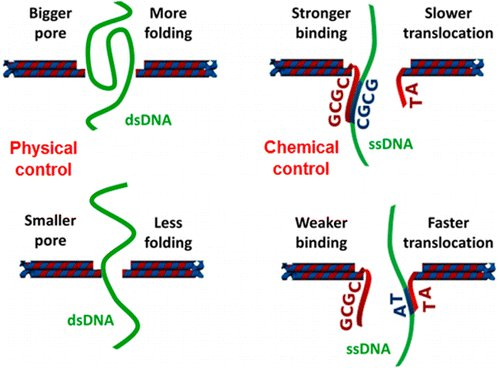
\includegraphics[width=0.8\textwidth]{origamitransloc.jpg}

\caption[Nanopore et origami d'ADN]{Un nanopore dans une membrane d'origami d'ADN \cite{HernndezAinsa2013}. Ce type de nanopore est de taille aisément adaptable et peut être fonctionnalisé facilement.}
\label{origamitransloc}
\end{center}
\end{figure}



Le fait de pouvoir travailler avec des membranes fines est une nouveauté qui laisse entrevoir une alternative à la mesure de courant ionique afin de déterminer la séquence de l'ADN en cours de translocation.





\newpage
\subsection{Mesures de courant et séquençage}

Comme nous l'avons vu précédemment, la mesure du courant ionique au cours de la translocation est l'idée maîtresse qui a guidé l'utilisation de nanopores afin de séquencer. Cependant l'arrivée des membranes fines laisse envisager une alternative: la mesure du courant transverse lors de la translocation. Illustrée sur la figure \ref{couranttransv1}


\begin{figure}[H]
\begin{center}
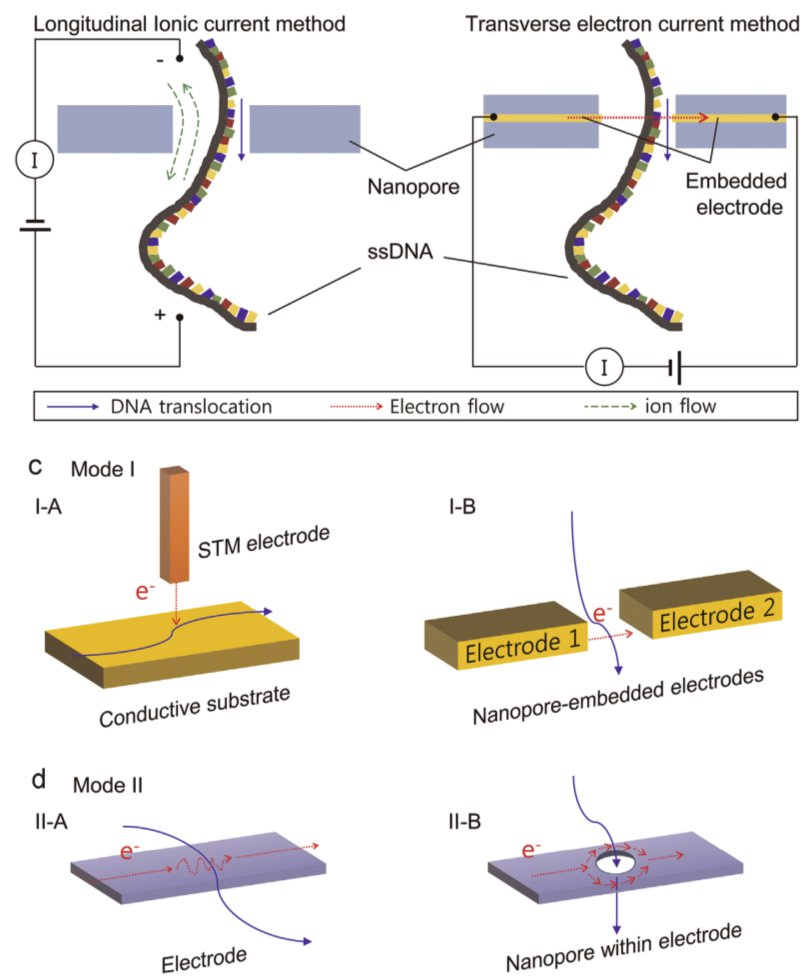
\includegraphics[width=0.8\textwidth]{introcouranttransverse.jpg}

\caption[Courants ioniques et transverses]{En plus de la mesure longitudiale du courant ionique lors de la translocation (a), il est possible avec les membranes fines de mesurer un courant électronique transverse (b) selon deux modes. Pour le premier mode (c), la translocation à lieu entre deux électrodes, alors que pour le deuxième mode (d), le nanopore est situé au sein d'une électrode.}
\label{couranttransv1}
\end{center}
\end{figure}

L'article de revue de Kim et al.\cite{Kim2015} présente plusieurs exemples de montages expérimentaux permettant de mesurer ce courant transverse (voir figure \ref{couranttransv2}). Les exemples donnés concernent le graphène mais il possible d'imaginer le même type de structure avec du sulfure de molybdène ou des origamis d'ADN dopés pour la conductivité.



\begin{figure}[H]
\begin{center}
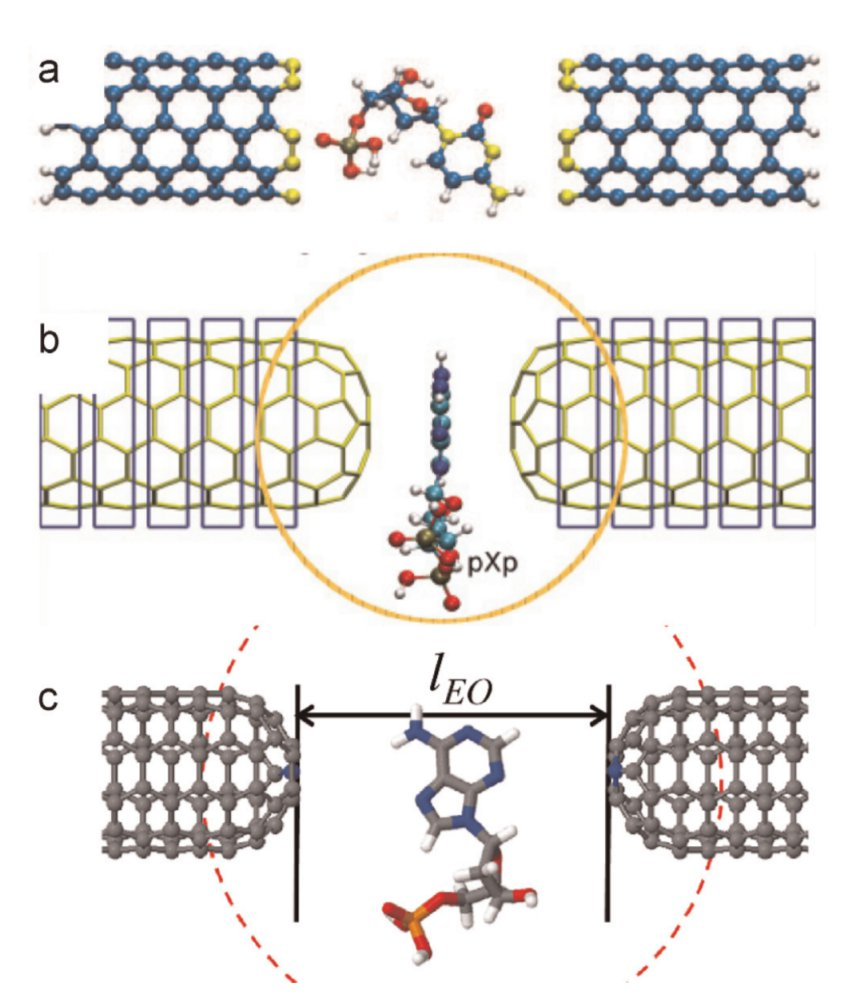
\includegraphics[width=0.7\textwidth]{couranttransv2.jpg}
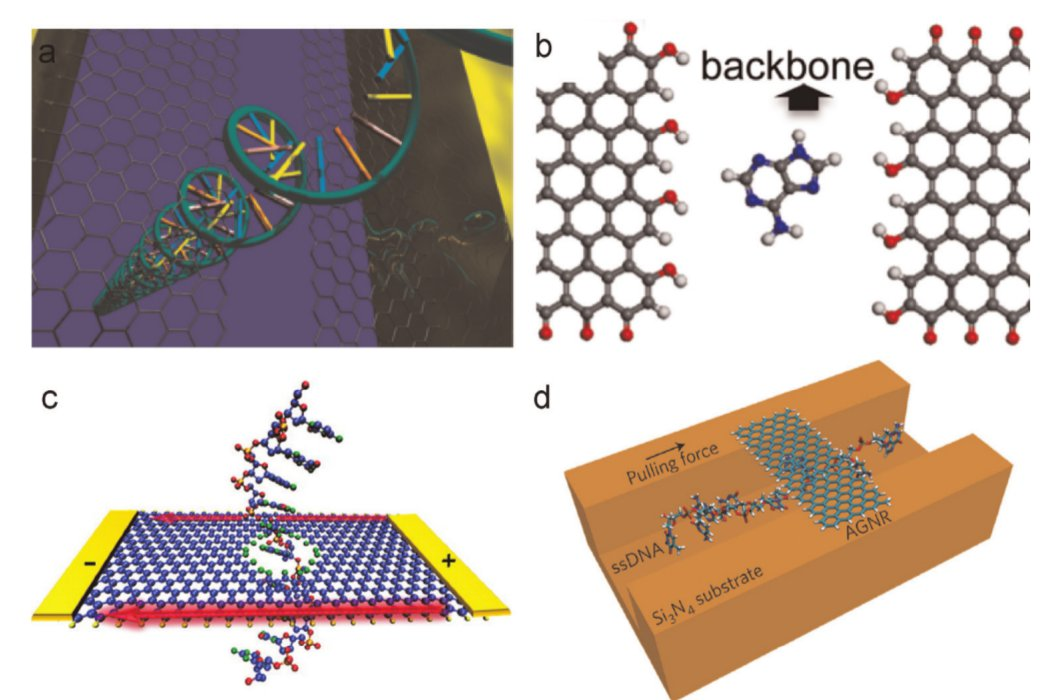
\includegraphics[width=0.7\textwidth]{couranttransv1.jpg}

\caption[Montages pour mesure du courant transverse]{Exemples de mesures de courant électroniques transverses lors de la translocation. En haut:  a/ membrane de graphène fonctionnalisée avec de l'azote \cite{Meunier2008} b/ nanotube de carbone utilisé comme membrane \cite{Chen2012} c/ nanotube de carbone fonctionnalisé avec de l'azote \cite{Kim2013}. En bas:  a/ nanopore constitué d'une bande \cite{Postma2010} b/ fonctionnalisation avec de l'oxygène \cite{Jeong2013} c/ nanopore au sein d'une électrode \cite{Saha2012} d/ Mesure de courant transverse perturbé par interactions orbitalaires \cite{Min2011}. Tous ces exemples concernent le premier mode sauf la figure c du bas qui montre un exemple de second mode.}
\label{couranttransv2}
\end{center}
\end{figure}







\section{Modélisation}


Après avoir vu le contexte technologique dans lequel s'inscrit le séquençage par nanopore, intéressons nous aux différentes manières de modéliser ce problème.





\subsection{Modèles théoriques}

Comme nous venons de le voir, l'utilisation de la translocation de l'ADN à des fins de séquençage est prometteur. Ce potentiel a créer un certain engouement au sein de la communauté scientifique. Dès 1996  Sung et Park proposent une première approche théorique de la translocation \cite{Sung1996} poursuivie en 1999 par Muthukumar \cite{Muthukumar1999}. Ils calculent une barrière d'énergie à franchir au cours de la translocation et proposent de résoudre l'équation de Fokker-Planck (propre des systèmes diffusifs \cite{shiriaev1992selected}). L'ADN, comme tout polymère, suit des lois générales de physique statistique (voir les travaux du prix Nobel Pierre-Gilles de Gennes \cite{Gennes197911} et notre \hyperref[resideal]{deuxième chapitre} qui y consacre une bonne partie), la difficulté réside dans le fait que pour la translocation, les conditions d'équilibres sont rarement remplies et de nombreuses tentatives d'explications théoriques ont eu lieu. Le \hyperref[translocmurfixe]{chapitre 3} consacre un long chapitre à toutes les théories développées afin de comprendre la translocation des polymères. Une approche théorique peut également être entreprise afin de prédire les courant ioniques au cours de la translocation \cite{Im2002,Noskov2004,Saraniti2006}. La comparaison aux expériences n'est pas toujours évidente et la mise en place de modèles numérique est nécessaire pour comprendre toutes les subtilités du problème.




\subsection{Echelles des modèles numériques}


Puisque l'ADN est un polymère  et en tant que tel suit des lois communes à tous les polymères, mais il présente également des propriétés qui lui sont propres. Pour attaquer le problème de la translocation, il faut d'abord choisir le niveau de détail souhaité. Si l'on souhaite comprendre le problème de la translocation de polymères en générale, des modèles simples, avec un faible niveau de détails, suffisent. Si l'on s'intéresse à la translocation d'une séquence particulière dans un pore ayant ses particularités, un niveau de détail fin, typiquement un modèle tout atomes, est nécessaire. De même si l'on souhaite déterminer le courant de translocation attendu. On peut également se situer à des échelles intermédiaires qui peuvent être un bon compromis, c'est le cas des modèles dit gros grains. La figure \ref{echellemodeles} présente trois modèles de niveaux de détails croissants.

\begin{figure}[H]
\begin{center}
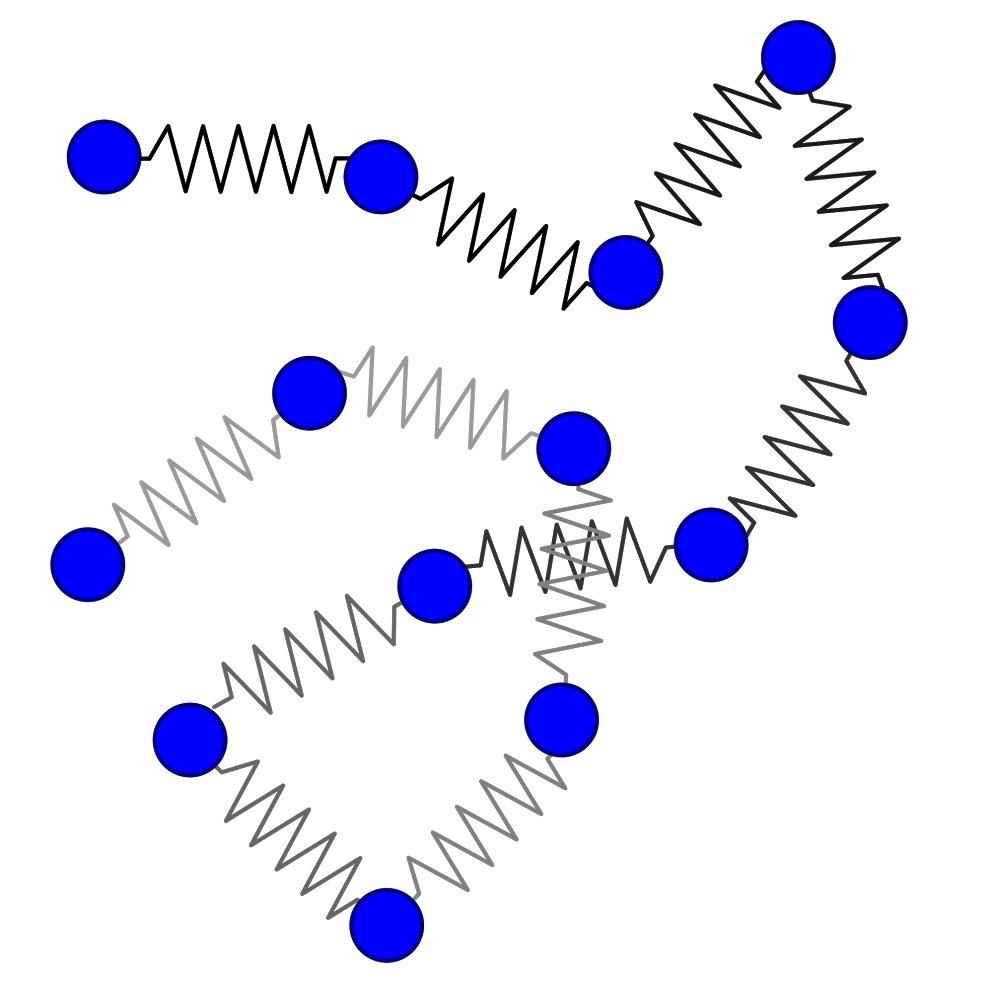
\includegraphics[width=0.3\textwidth]{beadspring.jpg}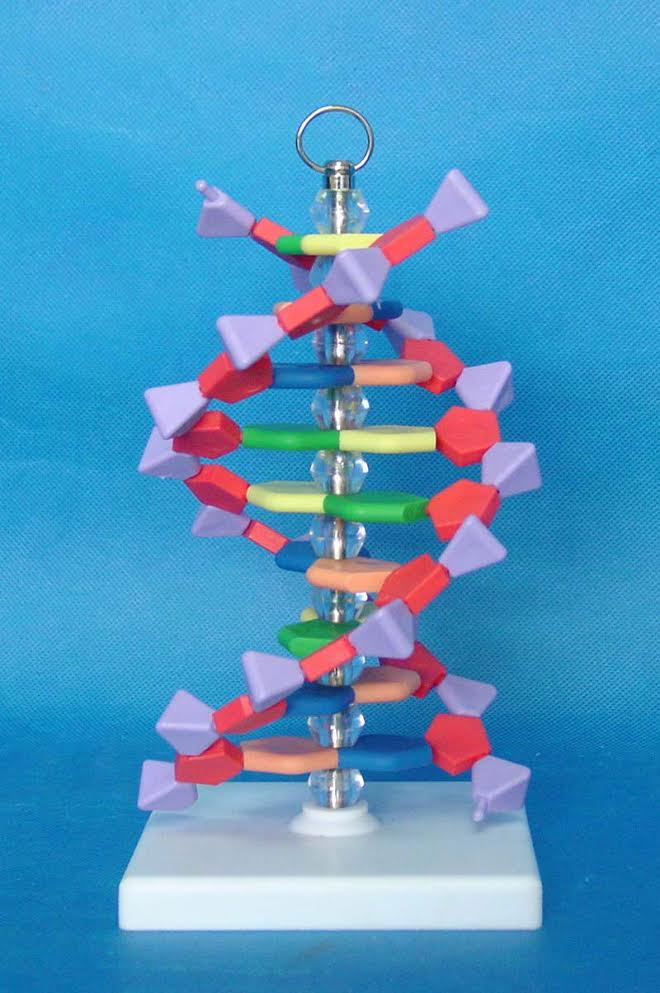
\includegraphics[width=0.21\textwidth]{coarsegraindnamodel.jpg}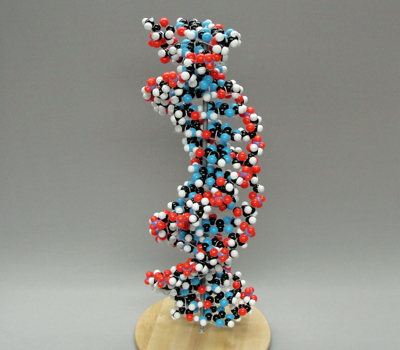
\includegraphics[width=0.36\textwidth]{fullatom.jpg}

\caption[Echelles de modèles]{Le modèle de Rouse \cite{Rouse1953} de niveau de détail faible est une simple succession de billes liées par des ressorts \cite{wikirouse}. Les modèles gros grains, rassemblant plusieurs atomes en une entité appelée grain présentent un niveau de détail intermédiaire \cite{coarsegrainmodna}. Le niveau de détail le plus fin est atteint par les modèles tout atomes \cite{fullatomdnamodel}.}
\label{echellemodeles}
\end{center}
\end{figure}



Le choix de l'échelle joue sur les comportements analysés. Un faible niveau de détail va faciliter l'obtention de lois de comportement générales car un ensemble statistique complet peut être investigué. En revanche si l'on souhaite regarder des propriétés particulières à certaines séquences d'ADN, un modèle à haute résolution est nécessaire. Une fois l'échelle choisie, il devient nécessaire d'employer un type de simulation adapté à cette échelle pour obtenir un modèle pertinent.


\subsection{Types de schémas numériques}

Il existe trois types de schémas numériques adaptés au problème de la translocation de polymères:
\begin{itemize}
\item Les méthodes de type Monte-Carlo
\item La Dynamique Moléculaire
\item Les simulations de type DFT (Density Functional Theory)

\end{itemize}

Chacun est adapté à certaines échelles et permet de vérifier des propriétés caractéristiques.\\

\subsubsection*{Les schémas numériques de type Monte-Carlo}  

Les méthodes de Monte-Carlo regroupent une large classe d'algorithmes de calculs qui se basent sur la répétition de tirages aléatoires pour obtenir des résultats numériques. Elles peuvent s'adapter à la résolution de tout problème probabiliste. La physique statistique des polymères donne un ensemble de loi probabilistes qui permettent d'intégrer des trajectoires de polymère par des algorithmes de type Monte-Carlo \cite{Verdier1962}. Typiquement, un maillage fin est réalisé dans le plan ou l'espace et un tirage de déplacements légers est imposé au parties constituante du polymère (voir figure \ref{montecarlotransloc}). Si l'énergie du nouveau tirage est inférieure à celle du précédent, il est conservé, sinon il est conservé avec une probabilité de $\exp(-\frac{\Delta H}{k_BT})$ ($H$ étant l'Hamiltonien du système) \cite{landau2009a}.

Ce type de modèle n'est efficace que pour un niveau de détails très faible et n'a été appliqué que pour des polymères linéaires simples. Les simulations de translocation de polymère par ces méthodes permettent de déterminer des comportements généraux (à travers des exposants critiques que nous définissons au \hyperref[taubiased]{chapitre 3}) \cite{Milchev2004,Kantor2004,2Luo2006,Tsuchiya2007,Dubbeldam2007}.



\begin{figure}[H]
\begin{center}
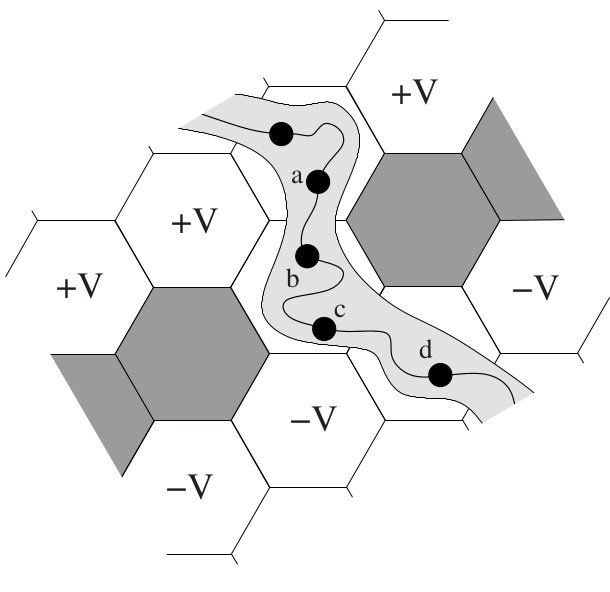
\includegraphics[width=0.6\textwidth]{montecarlotransloc.jpg}

\caption[Simulations de type Monte-Carlo]{Illustration d'un modèle de translocation de polymère résolu par une méthode de type Monte-Carlo \cite{these}. La translocation est biaisée par une différence de potentiel électrique, le polymère évolue dans un plan maillé par un réseau hexagonal.}
\label{montecarlotransloc}
\end{center}
\end{figure}





\subsubsection*{La Dynamique Moléculaire}

La dynamique moléculaire est une méthode de simulation numérique qui consiste en une intégration des équations du mouvement d'un système à N corps. Ces N corps (que l'on appellera grains) interagissent entre eux via des potentiels. Les équation de Newton sont ensuite résolues par un algorithme \cite{Verlet1967}. La force de la dynamique moléculaire est qu'elle peut s'adapter à toutes les échelles. En effet, si les N grains représentent des atomes, l'échelle tout atome est décrite, si ils représentent une chaîne d'oscillateurs couplés, un niveau de détail faible est modélisé et si ils représentent des molécules ou collections d'atomes, on obtient la description d'une échelle intermédiaire. Le problème de la translocation peut être abordé à n'importe quelle échelle grâce à la dynamique moléculaire.\\

Pour le niveau de détails le plus élevé, la première étape consiste à bien définir les interactions atomiques à l'aide d'un ensemble de champs de force moléculaires \cite{allen1987computer}. Ensuite il faut construire le système qui peut être, dans le cas du tout atome, identique aux conditions expérimentales \cite{Sathe2011,Farimani2014,Meunier2008,Chen2012,Kim2013,Postma2010,Jeong2013,Saha2012,Min2011,Aksimentiev2005,Aksimentiev2009,Heng2004,Heng2006}.
Bien que la précision soit alors très bonne, l'inconvénient de ce type de modèles est qu'il sont numériquement très gourmands en temps de calculs et les simulations sont donc limités à une échelle de temps réduite.

Des modèles simples, comme le modèle de Rouse par exemple peuvent également être utilisés pour déterminer des comportements généraux  \cite{Tian2003,Huopaniemi2006,Huopaniemi2007,Luo2008,Bhattacharya2009,Fyta2008,Luo2009,Ikonen2012}
(à l'instar des simulations de type Monte-Carlo). Nous allons nous même développer un modèle de polymère simple pour la translocation (voir \hyperref[porelargesimplepol]{chapitre 3}), avant d'augmenter le niveau de détails.

Il est possible de se situer entre ces deux échelles en utilisant des modèles dits gros grains. Les grains représentent alors un ensemble d'atomes. La translocation peut alors être abordée à l'échelle adaptée aux effets étudiés \cite{Forrey2007,Lansac2004,Ramachandran2011}. Nous utiliserons cette approche pour étudier la translocation d'un polymère structuré \hyperref[porelarge]{chapitre 3}.



\subsubsection*{La DFT}

La DFT n'est pas utilisée pour étudier la translocation a proprement parlé, elle est couplé à d'autres simulation afin de prédire les courants au cours de la translocation.





\cleardoublepage

\chapter{Modèle de polymères}
\label{polymerevalidation}

\cleardoublepage

{\Large\textbf{{Modèle de polymères}}}\\

\lettrine[loversize=0.6,lraise=0.1,findent=0.5em,nindent=0em]{D}{}ans ce chapitre, nous détaillons l'élaboration d'un modèle de polymères que nous utiliserons par la suite pour aborder la translocation. Nous avons opté pour un modèle gros grain et discutons de sa pertinence, des potentiels utilisés ainsi que des conditions dans lesquelles ont lieux les simulations. Ce modèle est ensuite testé et comparé à la théorie dans des situations statiques, dynamiques et de traction.\\

\minitoc

\begin{center}
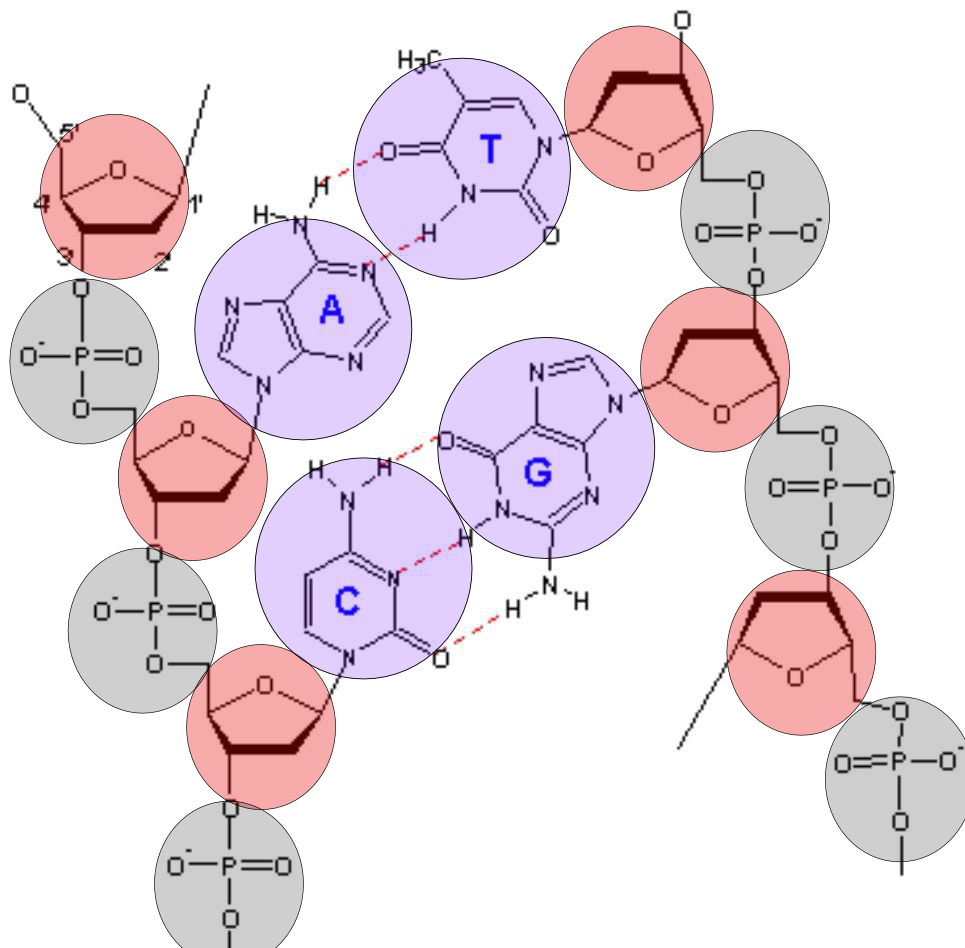
\includegraphics[width=0.7\textwidth]{coarsegraining.png}
\end{center}

\cleardoublepage







\section{Construction d'un modèle gros grain}

Comme nous l'avons vu dans le paragraphe précédent, l'utilisation de modèles gros grains, combinée à la dynamique moléculaire, permet de modéliser la translocation. Nous avons choisi cette méthode pour étudier le problème à une échelle qui n'a, à notre connaissance, pas encore était explorée. Nous nous proposons d'étudier un modèle suffisamment simple pour obtenir des résultats statistiquement pertinents, mais également suffisamment élaboré pour refléter certaines structures de l'ADN.

\subsection{Pertinence du modèle}
Avant même d'aborder le problème de la translocation, il est important de souligner la pertinence de l'utilisation de modèles gros grains et de la dynamique moléculaire dans l'étude de l'ADN. Comme nous l'avons signalé précédemment, une description du polymère prenant en compte tous les atomes est prohibitive en temps de calcul et inutile pour une analyse statistique complète. Il est donc nécessaire de rassembler plusieurs atomes dans un ensemble ( un grain) cohérent et de définir proprement les interactions entre ces ensembles. Rappelons que l'ADN est composé d'une chaîne principale, succession de phosphates et de sucres et de bases azotées greffées de manière latérale sur les sucres. Ces trois éléments sont des candidats idéaux pour une description de l'ADN constituée de trois types de grains, comme présenté sur la figure \ref{coarsegraindna}.

\begin{figure}[H]
\begin{center}
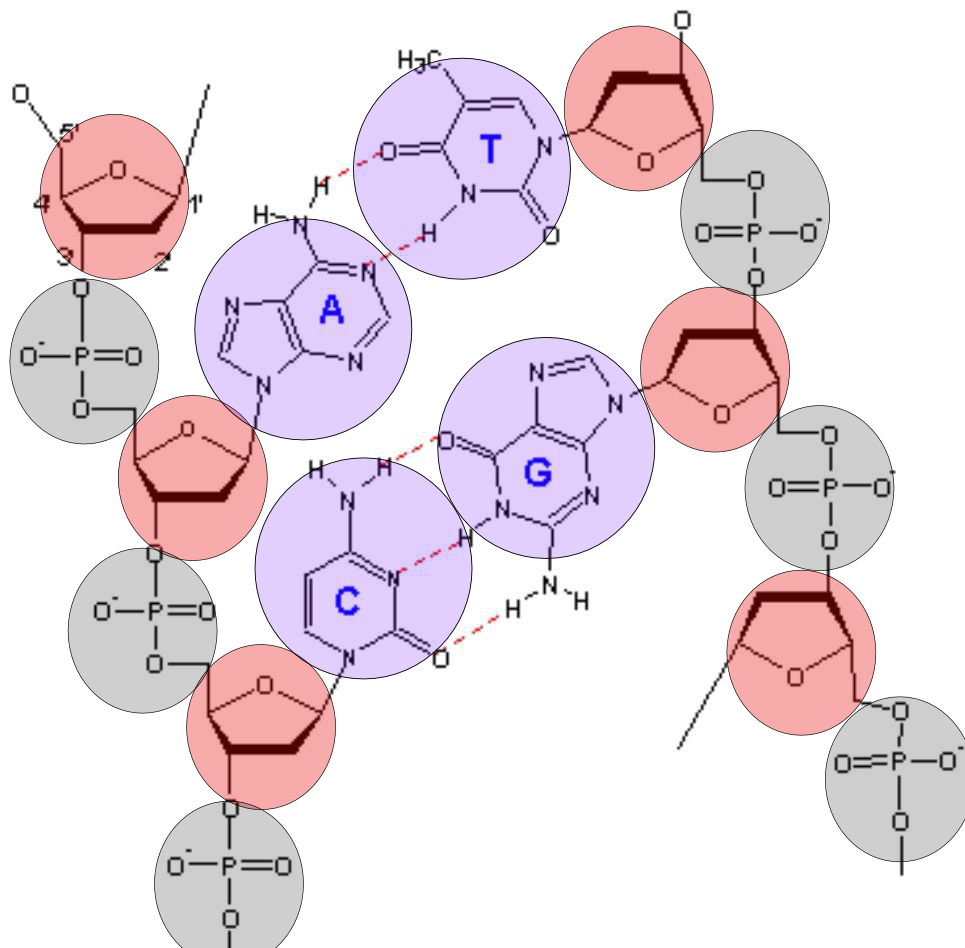
\includegraphics[width=0.65\textwidth]{coarsegraining.png}

\caption[Modèle gros grains]{Représentation gros grain de l'ADN. Trois types de grains représentant les phosphates, sucres et bases azotées composent un modèle d'ADN. De tailles proches, ces grains sont définis à partir d'éléments rigides et liés de manière covalente simple. Une fois la structure de grain définie, il faut définir leurs interactions.}
\label{coarsegraindna}
\end{center}
\end{figure}


En effet, plusieurs éléments justifient ce choix. Phosphate, sucres et bases azotées sont de tailles du même ordre de grandeur. Ils sont individuellement très peu déformables, de par sa géométrie pour le phosphate et par la présence de cycles rigides pour les sucres et les bases azotées. Les liaisons covalentes simples permettant une libre rotation sont situées entre ces grains. Une fois les grains choisis, il faut définir la manière dont ils interagissent entre eux. On définit donc des potentiels d’interaction. Pour l'ADN, on peut distinguer trois types de potentiels à définir: les interactions non spécifiques, la torsion au sein de la chaîne et les interactions entre bases azotées. Ces potentiels sont définis à partir d'étalons de distance ($\sigma$ et $R_0$) et d'énergie ($\epsilon$) qui traduisent les propriétés physiques du polymère. A partir de ces valeurs, on peut créer des échelles a-dimensionnées de temps, température, viscosité, force... On parle d'unités de Lennard-Jones. On discutera de la valeur de ces paramètres après avoir justifié les potentiels utilisés.


\subsection{Potentiels d'interaction}

\subsubsection{Interactions non spécifiques}

Il existe deux types d'interactions non spécifiques: les contacts entre grains et leurs liaisons. 

\begin{figure}[H]
\begin{center}
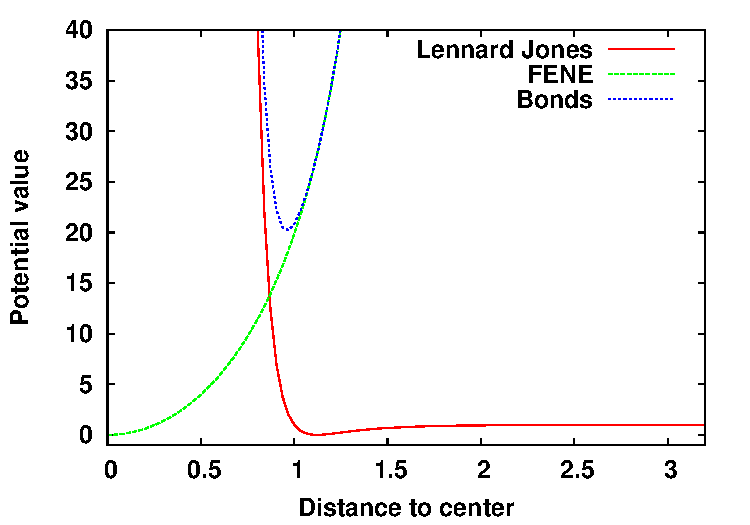
\includegraphics[width=0.75\textwidth]{nonspec.pdf}

\caption[Potentiels stériques]{interactions non spécifiques pour un modèle gros grain de bio-polymère. Le potentiel de Lennard-Jones représente les interactions de contacts stériques et de Van der Waals entre grains. Combiné avec un potentiel de type FENE, on obtient une bonne représentation de liaison covalente simple.}
\label{nonspecificinterac}
\end{center}
\end{figure}


Pour les contacts, nous avons choisi d'utiliser un potentiel de type Lennard-Jones (LJ) \cite{Jones1924}, très répandu dans la littérature du fait de son adéquation avec les résultats expérimentaux \cite{Bouanich1992}:

\begin{eqnarray}
U_{LJ}(r_{ij})= 4\epsilon_{ij} \left[\left(\frac{\sigma_{ij}}{r_{ij}}\right)^{12}-\left(\frac{\sigma_{ij}}{r_{ij}}\right)^{6}\right] + \epsilon_{ij} \text{ }, \text{ } U_{LJ}(r_{ij})=0 \text{ pour }  r_{ij}> 2^{1/6}\sigma_{ij}
\end{eqnarray}

\noindent $r_{ij}$ étant la distance entre les grains i et j, ce potentiel empêche l'interpénétration à faible distance. On définit une taille de grain $\sigma$ pour chaque type de grain, une taille moyenne est utilisée pour le contact de grains de tailles différentes ($\sigma_{ij}=\frac{\sigma_i+\sigma_j}{2}$). L'échelle d'énergie $\epsilon_{ij}$ sera dans notre cas toujours égal à $\epsilon$ quelque soient $i$ et $j$. ceci permettra de limiter le nombre de paramètres ajustables.

Les liaisons covalentes entre grains sont modélisées par un potentiel anharmonique de type FENE (Finitely Extensible Nonlinear Elastic) :
\begin{eqnarray}
U_{FENE}(r_{ij})= -15\epsilon \left(\frac{R_0}{\sigma_{ij}}\right)^2\text{ } \ln\left[1-\left(\frac{r_{ij}}{R_0}\right)^2\right]
\end{eqnarray}
Un développement limité montre le comportement harmonique à faible distance et le logarithme impose une extension maximale $R_0$ à la liaison, $R_0$ que nous avons pris égal à 1.5 la taille $\sigma$ moyenne des grains liés. Le potentiel FENE représentant la contribution attractive de la liaison covalente est utilisé en complément du potentiel de Lennard-Jones, répulsif à courte distance. Il en résulte une position d'équilibre très stable qui est caractéristique de la longueur de la liaison. Les potentiels des interactions non spécifiques sont tracés sur la figure \ref{nonspecificinterac}.

\subsubsection{Torsion et interactions entre bases}

Viennent ensuite les interactions spécifiques particulières à l'ADN. Au sein de la chaîne il y à une certaine rigidité qui peut être modélisée par un potentiel d'interaction à trois corps comme proposé par Linak, Tourdeau et Dorfman \cite{jchem}: 

\begin{eqnarray}
U_{BB}(\phi)= 12\epsilon \left( 1+cos(\phi)\right)^{2}
\end{eqnarray}

\noindent Avec $\epsilon$ une échelle d'énergie et $\phi$ l'angle formé dans l'axe Sucre-Phosphate-Sucre, la rigidité de la liaison est traduite par un angle d'équilibre de $\pi$, soit une chaîne droite, voir figure \ref{torsion}. La flexibilité de la chaîne est permise une dérivée second faible près de l'équilibre et un puit de potentiel assez large.

\begin{figure}[H]
\begin{center}
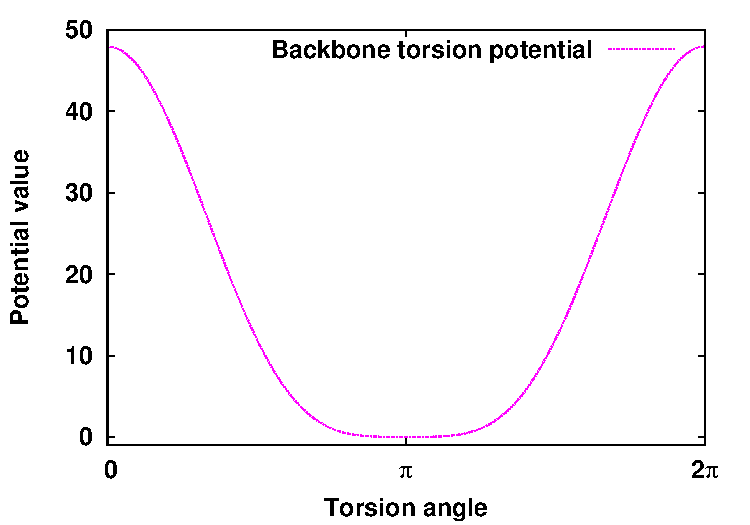
\includegraphics[width=0.7\textwidth]{backbone.pdf}

\caption[Potentiel de torsion]{La rigidité au sein de la chaîne peut être modélisée par un potentiel de torsion à trois corps. La position d'équilibre de $\pi$ favorise une chaîne linéaire mais le minimum peut prononcé, permet une certaine déformabilité pour les chaînes longues.}
\label{torsion}
\end{center}
\end{figure}

Parmi les interactions spécifiques, on identifie également les interactions entre bases azotées. Elles sont de deux types: liaisons hydrogènes et interactions orbitalaires directes ou croisées ($\pi$ stacking en anglais). Ces interactions peuvent (combinées à un potentiel de Lennard-Jones) être modélisées par le produit d'une fonction dépendante de la distance entre grains et d'une fonction caractéristique de leur orientation (avec un angle à définir). La figure \ref{hbonds} décrit un exemple de modélisation de ses interactions.


\begin{figure}[H]
\begin{center}
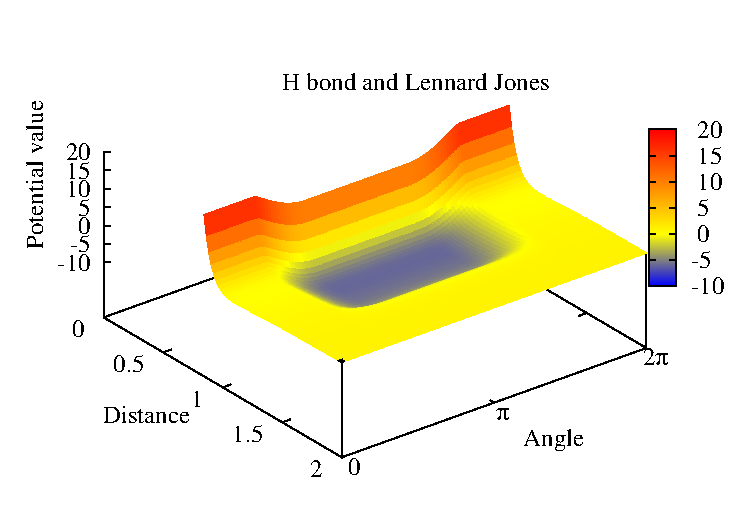
\includegraphics[width=0.9\textwidth]{bbhbonds.pdf}
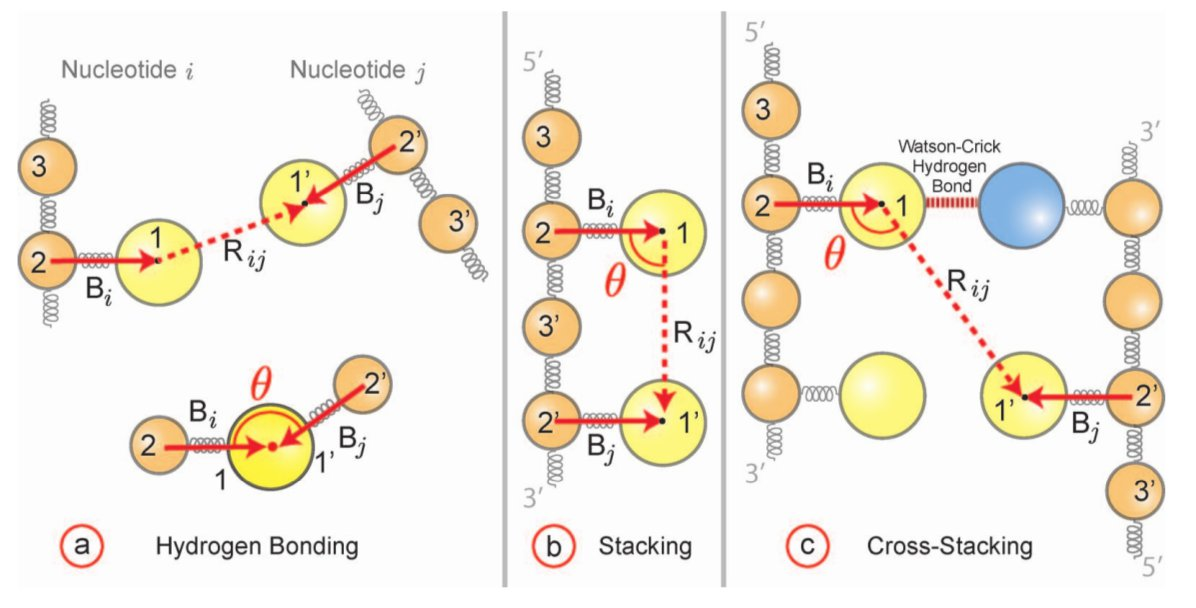
\includegraphics[width=0.9\textwidth]{specinterac.jpg}

\caption[Potentiels d'interaction spécifiques]{En haut: Exemple de potentiel permettant de décrire une liaison hydrogène. Le potentiel (auquel s'ajoute le potentiel de Lennard Jones) est modélisé par le produit d'une fonction caractéristique de l'éloignement des grains et d'une fonction représentant leur orientation. Le même type de potentiel peut être utilisé pour les interactions orbitalaires en définissant différemment l'angle de l'interaction. En bas: Exemple de définition d'angle \cite{jchem}.}
\label{hbonds}
\end{center}
\end{figure}

\subsubsection{Gains en coût de calcul}

Les potentiels décrits précédemment permettent de modéliser efficacement le comportement de l'ADN comme en attestent les travaux de Linak et al. \cite{jchem} qui décrivent l'ouverture d'épingles au sein de l'ADN ou le repliement d'un aptamère (petite séquence d'ADN synthétique capable de se fixer à un ligand spécifique). Cependant l'utilisation de potentiel élaborés augmente fortement le coût, en terme de calcul informatique, de résolution des trajectoires.

Ainsi, pour les potentiels simples à deux corps des interactions non spécifiques, il suffit de calculer la distance entre chaque couples de grains, une seule grandeur est calculée en une seule opération. On a alors un nombre de calculs à effectuer égal au nombre de paires possibles. Pour N grains on a alors un temps de calcul $\tau_c$ proportionnel à $N^2$ pour N grand comme le montre l'équation \ref{pairpot}.

\begin{eqnarray}
\tau_c(pairpotential) \propto \frac{N(N-1)}{2} \underset{N \rightarrow +\infty}{\sim} \frac{N^2}{2}
\label{pairpot}
\end{eqnarray}

On peut même utiliser pour N suffisamment grand des algorithmes plus efficaces basés sur l'utilisation de listes de plus proches voisins \cite{Vaidya1989} qui vont se comporter à l'infini en $O(Nln(N))$.

En ce qui concerne les potentiels à trois corps, le nombre de calculs nécessaires devient vite plus important. Ils nécessitent de définir un angle (il faut trois éléments pour cela). Le nombre d'opérations par rapport à une interaction non spécifique peut être identique, comme dans le cas du potentiel de torsion (uniquement le calcul de $cos(\theta)$ via un produit scalaire est nécessaire de par la symétrie du potentiel) ou doubler si le calcul de la distance est également nécessaire. On a alors un nombre de potentiels à calculer qui peut vite devenir prohibitif. Pour la torsion, le nombre de potentiels est lié au nombre de liaisons et va donc varier en $O(N)$. En ce qui concerne les interactions entre bases, avec un possible repliement du polymère et la création de structures en épingles, on a un nombre de potentiels à calculer proportionnel au nombre de triplets de grains représentant les bases et donc un temps de calcul décrit par l'équation \ref{3bodypot}, qui pourra éventuellement être amélioré par l'utilisation d'algorithmes de type liste de plus proches voisin, mais demeurant toujours extrêmement élevé.

\begin{eqnarray}
\tau_c(3bodypotential) \propto \frac{N(N-1)(N-2)}{6} \underset{+\infty}{\sim} \frac{N^3}{6}
\label{3bodypot}
\end{eqnarray}



Afin d'étudier la translocation de bio-polymères, nous allons utiliser des ADN simple brins et des chaînes relativement courtes, les potentiels d'interactions entre bases et de torsion en plus d'être gourmand en effort de calcul ne sont donc pas des plus pertinents. En effet, une chaîne courte représentera donc une tige rigide si on applique la torsion, on s'éloigne alors du problème réel. La différence de longueur de persistance pour un ADN simple brin reste limitée (de l'ordre de 1 à 2 bases), contrairement à la rigidité du double brin (longueur de persistance de l'ordre de 150 paires de bases) qui nécessite alors la prise en compte de la torsion. De plus nous n'avons pas pour objectif d'étudier les effets d'éventuelles épingles dans l'ADN sur la translocation, ce qui fait que des auto-interactions entre bases au sein du polymère ne sont pas non plus pertinentes.

Pour notre modèle de polymère, nous n'allons donc conserver que des interactions non spécifiques afin de créer un polymère simple mais structuré dans des proportions géométriquement proches de l'ADN. On aura uniquement des potentiels de type Lennard-Jones, éventuellement couplés à des potentiels de type FENE pour les liaisons covalentes entre grains.

\subsection{Conditions de simulation}

\subsubsection{Dynamique moléculaire et résolution des équations du mouvement}

Les potentiels choisis, il faut maintenant résoudre les trajectoires de translocation. Nous allons alors définir les conditions de simulation, les équations du mouvement à résoudre, les méthodes numériques utilisées et relier ce qui peut l'être aux conditions expérimentales.
Un fichier caractérisant le système ainsi qu'une liste d'instructions sont fournis à un solveur de dynamique moléculaire, LAMMPS \cite{lammps}, afin de réaliser nos simulations.

\subsubsection{Conditions thermodynamiques et équations du mouvement}



Pour résoudre nos trajectoires, nous nous plaçons dans l'ensemble canonique, nous travaillons donc avec un nombre de grains constant, un volume constant (avec des conditions aux limites périodiques) et température constante. La gravité, faible devant les autres grandeurs du problème n'est pas prise en compte.


Nous prenons en revanche en compte des interactions dont nous n'avons pas encore discuté, celles avec le solvant. Il est naturellement hors de question de représenter toutes les molécules de solvant et de calculer leurs trajectoires. Nous modéliserons la contribution du solvant de deux façons, une partie de frottement fluide (Stokes drag) qui représente le frottement et une partie de bruit thermique. 


%De plus, les dimensions nanométriques du systèmes impliquent un nombre de Reynolds\footnote{Le nombre de Reynolds est le rapport des échelles de temps caractéristiques inertielles et visqueuses.} très faible. On va donc négliger les termes inertiels des équations de Newton.

Nous obtenons ainsi pour les équations du mouvement appliquées à chacun des grains composants notre système, l'équation dite de Langevin \cite{Lemons1997} :

%dite de Langevin:
%\begin{eqnarray}
%\large{
%\frac{d \textbf{r}_n}{dt} = - \frac{1}{\nu_n}\frac{\partial U_{n}}{\partial \textbf{r}_n}   + \textbf{g}_n}
%\label{langevin}
%\end{eqnarray}
\begin{eqnarray}
\large{
m_n \frac{\partial^2 \textbf{r}_n}{\partial t^2} = -\frac{\partial U_{n}}{\partial \textbf{r}_n} - \nu_n \textbf{v}_n   + \textbf{g}_n}
\label{langevin}
\end{eqnarray}



Avec $\textbf{r}_n$ la position du grain $n$, $t$ le temps, $U_{n}$ la somme des différents potentiels appliqués au grain $n$, $\nu_n$ le coefficient de frottement de $n$ et $\textbf{g}_n$ la contribution brownienne au mouvement. Cette contribution brownienne présente les propriétés suivantes: sa moyenne est nulle, sa variance est proportionnelle à la température. C'est à dire:
\begin{eqnarray}
\left<\textbf{g}_n\right>\text{}=\text{} 0\text{ , } \left<\textbf{g}_n^2\right>\text{}=\text{} 2 k_B T\nu_n
\end{eqnarray}

 Notons que nous avons choisi de ne pas prendre en compte les interaction hydrodynamiques entre grains via le solvant (on en reparlera par la suite pour la théorie de la dynamique des polymères, voir figure \ref{hydrodyninterac}). De plus nous utiliserons une valeur $\nu_n$ identique pour chaque grain \\


\subsubsection{Paramètres du système et échelle d'unités réduites}

Nous avons défini la structure et les potentiels qui vont partiellement caractériser notre polymère, il reste à définir les paramètres et grandeurs physiques.

Pour les paramètres des potentiels conservés nous avons choisis les mêmes que Margaret C Linak et al. \cite{jchem} ont utilisé. La valeur de $\epsilon$ est fixée arbitrairement à 1 en unité LJ quelque soit le grain, en effet aucune contrainte sur l'échelle d'énergie ne s'applique pour l'instant. Par la suite, lorsque les unité ne seront pas explicitement précisées, elles seront en unité de Lennard-Jones. La taille d'un grain du squelette linéaire du polymère est prise pour référence: $\sigma=1$ correspondant à 0.3 nm pour de l'ADN. Les grains latéraux eux sont plus volumineux donc $\sigma_{L}=1.5$. Pour la distance maximale d'extension possible dans le potentiel de liaison FENE, $R_0=1.5\text{ } \sigma$ pour les liaisons du squelette et $R_0^{L}=1.5 \text{ }\frac{(\sigma+\sigma_{L})}{2} = 1.875\text{ } \sigma$. Pour la masse des grains, nous avons choisi  de simplifier le système en utilisant une même masse ($m$=1) pour tous les grains qui correspond alors à la masse moyenne des grains (1.6$\cdot 10^{-25} kg$, soit 100 fois la masse d'un atome d'hydrogène). La température que nous prendrons comme référence vaut 1.5 $\epsilon$ pour une température ambiante de 300 K. Le rapport des échelles de taille et d'énergie va nous donner une échelle de force ad-dimensionnée $\epsilon/\sigma$ dont l'unité correspond à 9.1 pN. De même, on peut définir une échelle de temps avec les échelles d'énergie, masse et de distance (voir tableau) pour obtenir une unité de temps de 1.3 ps. Le dernier paramètre qui va nous intéresser est le coefficient de frottement, caractéristique des interactions avec le solvant pour lequel on construit également une échelle.







\begin{table}
\setstretch{2}
\begin{center}
\begin{tabular}{|c|c|c|c|c|}
  \hline
  Quantité observée & Dimension & Symbol & Unité LJ & Valeur S.I. \\
  \hline
  Distance & $m$ & $\sigma$ & $\sigma$ & 0.3 nm\\
  Masse & $kg$ & $m$ & $m$ & 1.6$\cdot 10^{-25} kg$ \\
  Energie & $J$ & $\epsilon$ & $\epsilon$ & 2.74$\cdot 10^{-21} J$\\
  Température & $K$ & T & $\epsilon/k_B$ & 200 $K$\\
  Force & N  & F & $\epsilon/\sigma$ & 9.1$\cdot 10^{-12} N$ \\
  Temps & s & t ou $\tau$ & $\epsilon^{1/2} m^{-1/2} \sigma^{-1} $& 1.3$\cdot 10^{-12} s$\\
  Coefficient de frottement & $ m^3 J^{-1} s^{-1}$ & $ \nu$ & $ \sigma^4 \epsilon^{-3/2} m^{1/2}$ & 7.6$\cdot 10^{-9} m^3J^{-1}s^{-1}$\\
  
  \hline
\end{tabular}
\caption[Correspondance unités de Lennard Jones / S.I. ]{Correspondance entre les unités de Lennard Jones et du Système International}

\end{center}
\end{table}



On sera amenés par la suite à compléter ces paramètres et ce tableau en incluant les propriétés de la membrane à travers laquelle le polymère va effectuer une translocation et leurs interactions.

\section{Validation théorique du modèle}

\subsection{Statique. Polymères idéaux et non idéaux}

\subsubsection{Théorie}
Nous allons dans un premier temps présenter un modèle naïf de polymère idéal afin de poser les bases admises en physique des polymères \cite{Gennes197911,Flory195312,Doi199507,these}.\\

Le polymère évolue sur un réseau périodique de paramètre $\lambda$. La tête du polymère est placée sur un des nœuds du réseau. Les monomères consécutifs sont placés sur un des $z$ ($z=4$ pour un réseau carré à deux dimensions) sites plus proches voisins, le polymère réalise alors une marche aléatoire. Dans ce modèle de marche aléatoire simple, le marcheur ne se préoccupe pas de sa trajectoire passée qu'il peut éventuellement croiser (voir figure \ref{resideal}).

\begin{figure}[H]
\begin{center}
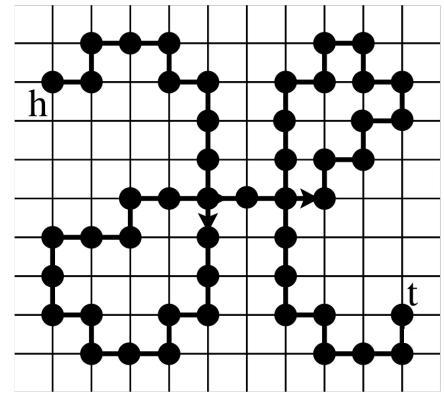
\includegraphics[width=0.45\textwidth]{resideal.jpg}

\caption[Marche aléatoire sur réseau]{Réseau carré montrant la marche aléatoire qui génère une configuration d'un polymère \cite{these}.}
\label{resideal}
\end{center}
\end{figure}

On déduit facilement que pour un degré de polymérisation $N+1$, il y a $Z_{ideal}=z^N$ polymères distincts possibles. Recalculons les résultats fondamentaux concernant la marche aléatoire génératrice du polymère. Ces résultats sont indépendants du réseau qui est un artifice de calcul et ne modifie pas les lois d'échelle. La plupart des modèles numériques n'utilisent pas de maillage. Soit $\textbf{r}$ le vecteur position du marcheur par rapport à l'origine et $b$ la taille d'un pas effectué par le marcheur. Soit $\textbf{r}_n$ le $n$-ième pas effectué, au bout d'un nombre de pas $N$, on a: 

\begin{eqnarray}
\textbf{r} = \sum_{n = 1}^{N} \textbf{r}_n
\end{eqnarray}

Pour la marche aléatoire idéale, il n'y a pas de corrélation entre les différents pas, ce qui mathématiquement se traduit par $\left<\textbf{r}_i \cdot \textbf{r}_j\right> = \delta_{i,j} b^2$. Ce qui implique les relations suivantes:

\begin{eqnarray}
\left<\textbf{r}\right>\text{} = \sum_{n = 1}^{N} \left<\textbf{r}_n \right>\text{} =\text{} 0 \text{ }, \text{} \left<\textbf{r}^2\right> \text{}= \sum_{i = 1}^{N} \sum_{j = 1}^{N} \left<\textbf{r}_i \cdot \textbf{r}_j\right> \text{}= \sum_{i = 1}^{N} \left<\textbf{r}_i^2\right> \text{}= b^2 N
\label{rdmwalk}
\end{eqnarray}

 Puisque la valeur moyenne de $\textbf{r}$ est nulle, on estime le comportement de la distance entre les extrémités (distance bout-à-bout) moyenne du polymère en prenant la racine carré de la valeur moyenne de $\textbf{r}^2$. Comme le montre l'équation \ref{rdmwalk} la taille du polymère sera proportionnelle à $N^\frac{1}{2}$.\\
 
 Une estimation correcte de la taille du polymère est obtenue en considérant le rayon de giration $R_g$. Il est défini de la manière suivante en notant $\textbf{r}_{CM}$ la position du centre de masse du polymère :
 \begin{eqnarray}
R_g^2\text{}=\text{}\frac{1}{N}\sum_{n = 1}^{N} \left<(\textbf{r}_n-\textbf{r}_{CM})^2\right>
\label{equ}
\end{eqnarray}
 Avec $\textbf{r}_{CM}=\frac{1}{N}\sum_{n = 1}^{N} \textbf{r}_n$, ou encore, de manière équivalente: 
  \begin{eqnarray}
R_g^2\text{}=\text{}\frac{1}{2N^2}\sum_{i,j}^N \left<(\textbf{r}_i-\textbf{r}_{j})^2\right>
\label{equbthnth}
\end{eqnarray}
 
 \noindent L'équivalence s'obtient en développant les termes des deux expressions et en les identifiant.\\


On va appliquer la dernière partie de l'équation \ref{rdmwalk} pour la marche aléatoire à l'équation \ref{equ} du rayon de giration en notant le fait qu'on effectue une marche aléatoire de $|i-j|$ pas pour aller du monomère $i$ au $j$ dans l'expression $\left<(\textbf{r}_i - \textbf{r}_j)^2\right>$.

\begin{gather}
R_g^2\text{}=\text{}\frac{1}{2N^2}\sum_{[|i-j|]} |i-j| b^2=\text{}\frac{1}{N^2}\sum_{[i>j]} |i-j| b^2\nonumber \\
=\text{}\frac{b^2}{N^2} \sum_{i=1}^N \sum_{j=1}^{i} j \\
 = \text{}\frac{b^2}{N^2}[\frac{1}{2}(\frac{N(N+1)(2N+1)}{6}+\frac{N(N+1)}{2})]\nonumber
\label{equationgyr}
\end{gather}

En prenant la limite $N \gg 1$ dans l'équation précédente, on obtient la loi d'échelle à laquelle le rayon de giration obéit:
\begin{eqnarray}
R_g^2\text{}\sim\text{}\frac{b^2}{6}N \Rightarrow R_g\propto N^{\frac12}
\end{eqnarray}

La distance bout-à-bout et le rayon de giration obéissent à la même loi d'échelle et sont caractéristiques de l'expansion spatiale du polymère.\\


Revenons à notre modèle sur réseau afin d'établir une équation différentielle sur la probabilité, $P(\textbf{r},N)$, du $N$-ième monomère d'être en $\textbf{r}$ (avec le premier monomère à l'origine). Pour cela, introduisons les z $\textbf{b}_i$  vecteurs les plus proches de la position $\textbf{r}$ pour obtenir:
\begin{eqnarray}
P(\textbf{r},N)= \frac{1}{z}\sum_{i=1}^{z} \left[P(\textbf{r}-\textbf{b}_i,N-1)\right]
\label{eqdifprob}
\end{eqnarray}

On effectue ensuite un développement limité à l'ordre 2 afin d'obtenir une équation différentielle à résoudre sur la probabilité de distribution. Avec pour hypothèse que $\textbf{r}\gg\textbf{b}_i$ et $N \gg 1$.

\begin{eqnarray}
P(\textbf{r}-\textbf{b}_i,N-1)=P(\textbf{r},N)- \frac{\partial P}{\partial N}-  \textbf{b}_{i\alpha} \frac{\partial P}{\partial r_{\alpha} } + \frac12 \textbf{b}_{i\alpha}\textbf{b}_{i\beta} \frac{\partial ^2 P}{\partial r_{\alpha}\partial r_{\beta} }
\end{eqnarray}

En utilisant la convention de sommation d'Einstein, $i$ varie de $1$ à $z$ et $\alpha$ et $\beta$ représentent les coordonnées spatiales. En considérant les résultats suivants:

\begin{eqnarray}
\sum_{i=1}^{z}\textbf{b}_{i\alpha}=0 \text{ },\text{ } \sum_{i=1}^{z}\textbf{b}_{i\alpha}\cdot\textbf{b}_{i\beta} = \frac{b^2\delta_{\alpha,\beta}}{3}
\end{eqnarray}

On obtient l'équation différentielle qui régit la probabilité de distribution de nos monomères:
\begin{eqnarray}
 \frac{\partial P}{\partial N} =   \frac{b^2}{6}\frac{\partial ^2 P}{\partial ^2 \textbf{r}}
 \label{eqdif}
\end{eqnarray}

Cette équation différentielle (\ref{eqdif}) a pour solution avec pour condition initiale $\textbf{r}=0$ quand $N=0$ :
\begin{eqnarray}
P(\textbf{r},N)=\left(\frac{3}{2\pi N b^2}\right)^\frac{3}{2}\exp\left(-\frac{3\textbf{r}^2}{2 N b^2}\right)
\end{eqnarray}

La distribution de probabilité de présence des monomères est donc gaussienne, un polymère idéal est d'ailleurs souvent dit gaussien.\\

Remarquons dors et déjà que le logarithme de la distribution de probabilité donne par définition l'énergie libre du système qui n'est pas sans rappeler celle d'un ressort:
\begin{eqnarray}
F(\textbf{r})= - k_B T \ln(P(\textbf{r},N))= F(0)+\frac{3k_BTr^2}{2Nb^2}
\label{elibre}
\end{eqnarray}
$k_B$ est la constante de Boltzmann. Cette énergie sera utilisée par la suite pour décrire des propriétés dynamiques du polymère.\\



Bien entendu ce modèle est simpliste, un vrai polymère ne peut en aucun cas s'auto-intersecter, il peut ne pas être linéaire...\\

 Traitons le cas d'un polymère qui ne peut s'intersecter lui-même. Les configurations sont alors générées par des marches aléatoires auto-évitantes (Self Avoiding Walks ou SAW). Soit $v_c \propto b^3$ le volume exclusif occupé par un monomère. La probabilité qu'un monomère de la chaîne de volume $R^3$ ne se superpose pas à un autre est $(1-v_c/R^3)$, il y a $\frac{1}{2}N(N-1)$ paires de monomères. La probabilité totale de non superposition est donc:
 \begin{eqnarray}
P_{ns}(N)= \left(1-\frac{v_c}{R^3}\right)^{\frac{N(N-1)}{2}} = \exp\left[\frac{N(N-1)}{2}\text{ }\ln\left(1-\frac{v_c}{R^3}\right)\right]
\end{eqnarray}

La probabilité de distribution d'une SAW est donc le produit des deux probabilités précédentes, ce qui donne dans la limite $N \gg 1$, $R \gg v_c$:
\begin{eqnarray}
P_{SAW}(R,N)=P_{ns}(N) P(R,N)=\exp\left[-\frac{3R^2}{2 N b^2}-\frac{v_cN^2}{2R^3}\right]
\end{eqnarray}

La taille caractéristique du polymère est alors donnée par la valeur $R^*$ qui maximise la probabilité de distribution, d'où:

\begin{gather}
\frac{\partial P_{SAW}(R,N)}{\partial R} \Huge{|} _{R=R^*}=0 \nonumber\\
\Rightarrow \frac{3R^{*2}}{Nb^2}-\frac{3v_cN}{2R^{*4}} =0 \\
\Rightarrow R^* \propto N^\frac{3}{5}\nonumber
\end{gather}


La taille caractéristique du polymère croit donc plus rapidement avec le nombre de monomères que dans le cas idéal précédent. L'exposant 3/5 trouvé est très proche de l'exposant de Flory, $\nu=0.588$, qui fait consensus parmi les différentes simulations numériques. \\


Le cas de la chaîne auto évitante est adapté aux polymères dilués en solution. Le modèle de la chaîne idéale décrit paradoxalement très bien un contexte de polymères en forte concentration en contacte les uns des autres. En effet les termes de volumes exclus s'appliquent pour le polymère aussi bien pour sa propre chaîne que pour la présence de chaînes voisines. L'espace précédemment libre est occupé, le volume exclu apporte une contribution énergétique uniforme dans tout l'espace. Les termes de volumes exclus se compensent donc tous, ce qui permet de se retrouver uniquement avec la contribution d'une chaîne idéale.

Comparons ces prédictions théorique à nos résultats numériques.

\subsubsection{Résultats numériques}
Pour tous les résultats que nous présentons, ici et par la suite, les barres d'erreurs sur la moyenne d'une valeur $A$ sont calculées avec l'équation \ref{errorbar}, $M$ étant le nombre de mesures de la valeur $A$.

\begin{eqnarray}
\sigma=\sqrt{\frac{\left<A^2\right>-\left<A\right>^2}{M}}
\label{errorbar}
\end{eqnarray}

De plus quand nous parlerons de la taille $N$ d'un polymère, nous parlerons d'un polymère ayant une chaîne comprenant $N$ grains. Il y a donc $N$ monomères consécutifs pour les modèles simples. Pour le modèle structuré, nous avons choisi de le symétriser (pour pouvoir par la suite redéfinir une des extrémité à laquelle on va appliquer une force). On a alors un nombre impair $N$ de grains formant la chaîne et $(N-1)/2$ grains latéraux.\\


Dans cette partie concernant la statique des polymères, nous avons observé les valeurs de la distance bout-à-bout et du rayon de giration pour des polymères laissés libres d'évoluer sans contraintes dans un milieu vide (Les interactions avec le solvant demeurent). Nous avons étudié en plus de notre système structuré, des polymères linéaires dont un polymère idéal (les seuls potentiels utilisés sont LJ et FENE uniquement pour les liaisons, l'interpénétration est possible entre grains non liés) et un polymère présentant des volumes exclus \footnote{Modèles réalisés par Gaël Radou lors d'un stage de Master 2 avant mon arrivée au laboratoire.}. Les valeurs des exposants caractéristiques sont légèrement supérieures en raison de la taille finie des modèles. En ce qui concerne notre modèle, nous nous attendons aussi à une valeur plus élevée. En effet les même sources d'augmentation sont présentes. De plus, la présence d'un grain latéral sur le squelette linéaire va augmenter la rigidité de notre polymère. Cette rigidité supplémentaire va augmenter les effets de taille fini. Le squelette sera alors plus longiligne, ce qui aura pour effet d'augmenter plus fortement sa taille effective lorsque $N$ croît. Comme le montre la figure  \ref{statiquenum}, dans le cas d'un polymère idéal, pour la distance bout-à-bout comme pour le rayon de giration, on approche la valeur théorique de $R\propto N^\frac{1}{2}$ par le haut ($R\propto N^{0.529}$ et $R_G\propto N^{0.512}$ respectivement). Pour le polymère linéaire avec volumes exclus, on trouve des valeurs de $\nu$, l'exposant de Flory, plus élevées ($R_G \propto N^{0.639}$) pour les raisons que nous avons avancées et ces valeurs sont encore plus augmentées dans le cas du polymère structuré ($R\propto N^{0.706}$ et $R_G \propto N^{0.697}$). \\


\begin{figure}[H]
\begin{center}
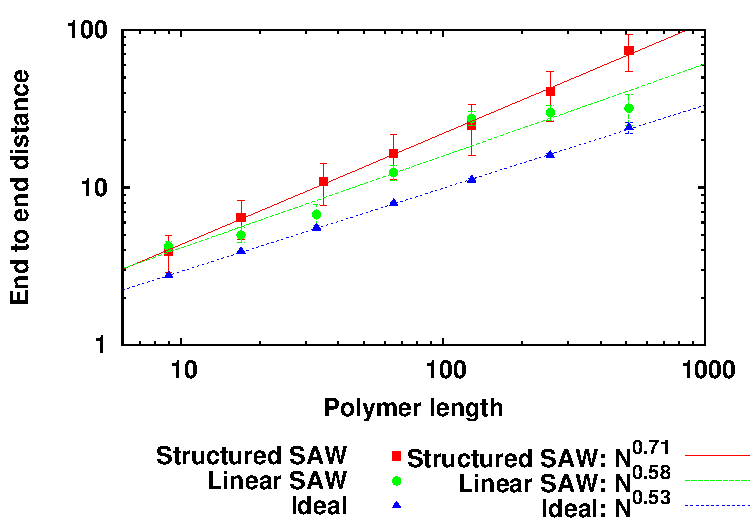
\includegraphics[width=0.9\textwidth]{endtoenddistance.pdf}

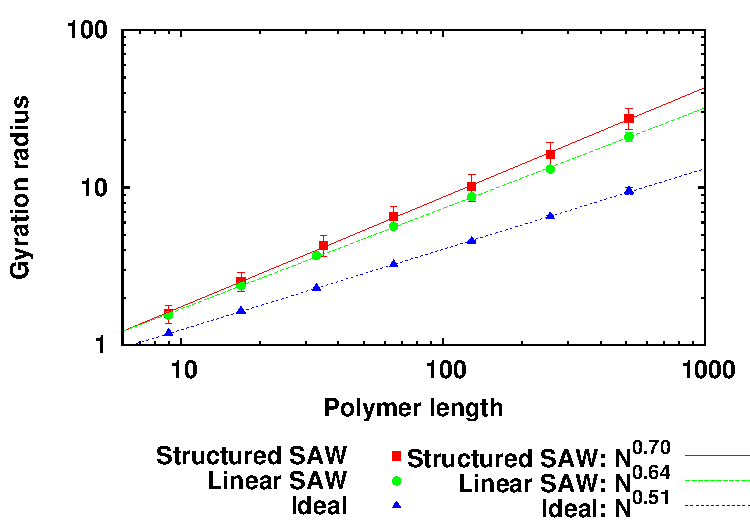
\includegraphics[width=0.9\textwidth]{gyration.pdf}

\caption[Résultats numériques: caractéristiques statiques.]{En haut: évolution de la distance bout-à-bout du polymère. En bas: évolution du rayon de giration du polymère. Des effets de tailles finies, amplifiés par une rigidité accrue dans le cas du polymère structuré, entraînent une estimation surévaluée des exposants prévus, mais ces derniers sont en bon accord avec la théorie. D'un point de vue statique, les différents modèles de polymères ont un comportement tout à fait normal.}
\label{statiquenum}
\end{center}
\end{figure}

\subsection{Dynamique des polymères}
\subsubsection{Théorie}

Nous allons maintenant proposer un modèle permettant d'aborder la dynamique d'une chaîne. Il s'agit du modèle de Rouse \cite{Rouse1953} (Figure \ref{rouse}). Comme nous l'avions signalé, l'énergie libre d'un polymère idéal présente les caractéristiques d'un potentiel harmonique de type ressort (cf: équation \ref{elibre}), ce qui justifie cette modélisation.

\begin{figure}[H]
\begin{center}
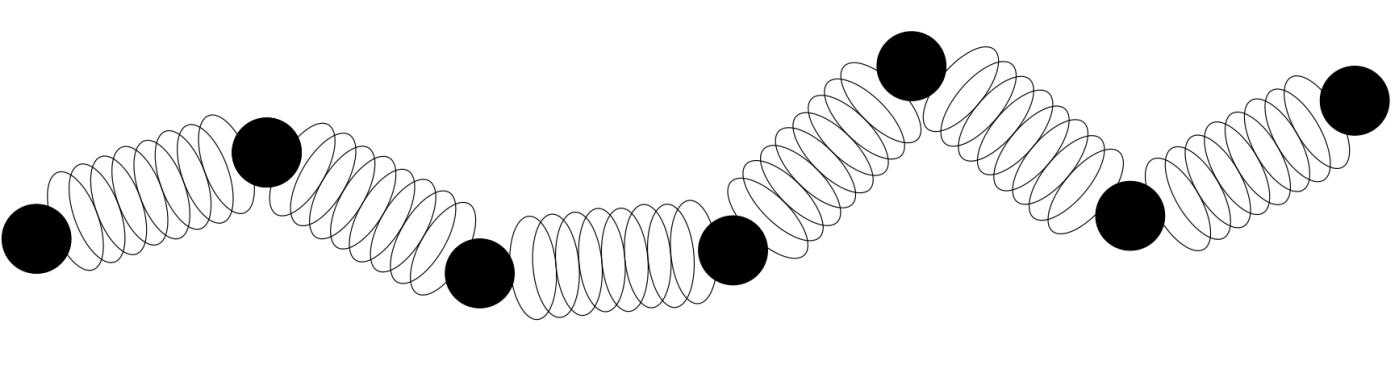
\includegraphics[width=0.8\textwidth]{rouse.jpg}

\caption[Modèle de Rouse]{Modélisation du polymère par une chaîne d'oscillateurs \cite{these}, appelé modèle de Rouse.}
\label{rouse}
\end{center}
\end{figure}

Le polymère est modélisé par une chaîne d'oscillateurs (de type billes/ressorts). Physiquement, le ressort ne représente pas une liaison entre monomères mais plutôt une partie du polymère assez longue pour que la statistique gaussienne puisse lui être appliquée. De l'équation \ref{elibre} obtenue précédemment on déduit l'énergie élastique du ressort connectant les billes $n$ et $n+1$ séparées par une distance d'équilibre moyenne $b$:


\begin{eqnarray}
F_{n,n+1} = \frac{3 k_B T}{2} \frac{(\textbf{r}_{n+1}-\textbf{r}_n)^2}{b^2}
\end{eqnarray}

Nous nous plaçons dans des conditions simples en modélisant l'effet du solvant par un simple terme de frottement visqueux (ou Stokes drag), la trajectoire est donc donnée par l'équation de Langevin ( \ref{langevin}). De plus, les dimensions nanométriques du systèmes impliquent un nombre de Reynolds\footnote{Le nombre de Reynolds est le rapport des échelles de temps caractéristiques inertielles et visqueuses.} très faible. On va donc négliger les termes inertiels dans l'équation de Langevin qui s'écrit ici:

\begin{eqnarray}
\large{
\frac{d \textbf{r}_n}{dt} =  \frac{3k_BT}{\nu_n b^2}( \textbf{r}_{n+1} +\textbf{r}_{n-1} -2\textbf{r}_n )  + \textbf{g}_n}
\end{eqnarray}

On va résoudre cette équation en prenant $n$ comme variable continue.

\begin{eqnarray}
\large{
\frac{d \textbf{r}}{dt} =  \frac{3k_BT}{\nu b^2}\frac{\partial ^2 \textbf{r}}{\partial  n^2} + \textbf{g}_n}
\end{eqnarray}

Avec les conditions limites $\frac{\partial  \textbf{r}}{\partial  n}=0$ en bouts de chaîne, on peut résoudre le système en le séparant en plusieurs modes à  partir de coordonnées normalisées: 
\begin{eqnarray}
\textbf{x}_p= \frac{1}{N} \int_0^N \cos \left(\frac{n\pi p}{N}\right) \text{ }\textbf{r}(n,t)\text{ } dn \text{ , } \frac{d \textbf{x}_p}{dt} =  -\frac{k_p}{\nu _p} \textbf{x}_p + \textbf{g}_p
\end{eqnarray}



\begin{eqnarray}
\nu_0=  N \nu \text{ , } \nu_p= 2 N \nu  \text{ , }  k_p=\frac{6k_BT\pi^2 p^2}{N b^2}  \text{ , }  \left<\textbf{g}_{p\alpha}(t) \cdot \textbf{g}_{q\beta}(t')\right> = 2\delta_{p,q} \delta_{\alpha ,\beta} \frac{k_BT}{\nu_p} \delta(t-t')
\end{eqnarray}

En travaillant dans la nouvelle base orthogonale, on peut montrer que:


\begin{eqnarray}
\left<(\textbf{x}_{0}(t)-\textbf{x}_{0}(0))_\alpha \cdot (\textbf{x}_{0}(t)-\textbf{x}_{0}(0))_\beta \right> = 2 \delta_{\alpha ,\beta} \frac{k_BT}{N\nu}t
\end{eqnarray}

\begin{eqnarray}
\left<\textbf{x}_{p\alpha}(t) \cdot \textbf{x}_{q\beta}(0)\right> = 2\delta_{p,q} \delta_{\alpha ,\beta} \frac{k_BT}{k_p} \exp\left(-\frac{t}{\tau_p}\right) \text{ , } \tau _p = \frac{\nu N^2 b^2}{3\pi^2p^2k_BT}
\end{eqnarray}

La distance bout-à-bout et le rayon de giration sont des combinaisons linéaires des $\textbf{x}_p$ et sont donc assujettis  au temps de relaxation le plus long, $\tau_1$ qui obéit à la loi d'échelle : $\tau_1 \propto N^2$. De même la position du centre de masse est donnée par $\textbf{x}_0$, ce qui permet d'en déduire le coefficient de diffusion du polymère:


\begin{eqnarray}
\left<(\textbf{r}_{CM}(t)-\textbf{r}_{CM}(0))^2\right>=\frac{6 k_B T}{N \nu} t = 6 D_R t
\label{fluctudissip}
\end{eqnarray}




L'équation précédente (\ref{fluctudissip}) traduit le théorème de fluctuation dissipation  en prenant en compte $N \nu$, le coefficient de Stokes global du polymère. Le temps de relaxation peut également être vu comme le temps mis par le centre de masse pour parcourir sa longueur.

 Le temps nécessaire au parcours d'une certaine distance est indépendant de la présence d'interactions entre monomères (chaîne idéale ou SAW), mais la longueur du polymère dépend des conditions du modèle. On a alors $\tau \propto \frac{R^2}{D}$, soit $\tau \propto N^2 $ dans le cas idéal ou $\tau \propto N^{1+2\nu} $ dans le cas de la marche auto-évitante. 

Expérimentalement, on ne retrouve pas ces résultats car le modèle néglige les interactions hydrodynamiques, des interactions à longue portée entre les monomères via le solvant. La figure \ref{hydrodyninterac} illustre ce phénomène. Le modèle de Rouse complété par l'ajout d'interactions hydro- dynamiques s’appelle le modèle de Zimm \cite{Zimm1956}.


\begin{figure}[H]
\begin{center}
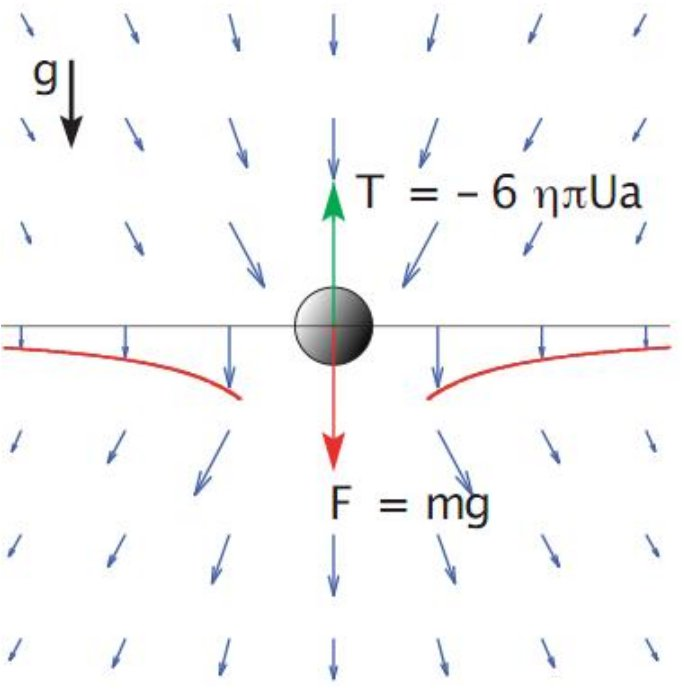
\includegraphics[width=0.4\textwidth]{hydrodyninterac.jpg} 

\caption[Interactions hydrodynamiques]{Mouvement de fluide généré par une bille en chute libre. Pour chaque objet en mouvement, le fluide déplacé génère un champ de vitesse, ces champs de vitesse décroissent en l'inverse de la distance et se superposent, il y a advection des objets par le fluide. Illustration de Bloen Metzger \cite{bloen}.}
\label{hydrodyninterac}
\end{center}
\end{figure}

La compréhension de la dynamique des polymères permet de s'attaquer à l'élaboration de modèles pour la translocation comme nous l'avons vu précédemment.


\subsubsection{Résultats numériques}



Afin de connaître l'évolution de la taille de notre système avec le nombre de monomères nous avons laissé évoluer librement notre polymère pendant un nombre important de pas de dynamique moléculaire (jusqu'au milliard pour les chaînes les plus longues). Cela génère un nombre important de configurations du polymère à l'équilibre. Toutefois, ces configurations ne sont pas indépendantes les unes des autres.\\

Pour connaître l'indépendance de nos configurations, nous avons défini une fonction d'auto-corrélation, $G(H,\tau)$ qui dépend d'une observable $H$ et du temps $\tau$ écoulé entre deux mesures de cette observable.
\begin{eqnarray}
G(H,\tau)=\frac{\left<H(t+\tau)H(t)\right> -\left<H(t)\right>^2}{\left<H(t)^2\right> -\left<H(t)\right> ^2}
\end{eqnarray}

Un script en langage C a été utilisé afin de calculer la fonction d'auto-corrélation pour le rayon de giration et la distance bout-à-bout à partir des données brutes générées par LAMMPS. Dans un premier temps la moyenne et la variance de l'observable sont calculées. Ensuite, un balayage avec une fenêtre de largeur glissante est effectué avec plusieurs valeurs de $\tau$ afin de calculer la quantité $\left<H(t+\tau)H(t)\right>$. Un fit exponentiel est alors effectué afin de déterminer un temps de corrélation. La figure \ref{correl} présente $G(R,\tau)$ du rayon de giration et de la distance bout-à-bout pour différentes tailles de chaîne. Une fois ces temps de corrélation défini, nous pouvons nous intéresser à leur évolution en fonction de la taille de notre polymère.

Le fit exponentiel n'est pas toujours parfait, notamment dans la zone des corrélations fortes, mais il a le mérite d'être une bonne définition du temps de corrélation car au bout de 5 $\tau_c$, la corrélation entre les différentes valeurs des mesures que nous avons prises est nulle. On utilise donc ce fit exponentiel pour estimer nos temps de corrélation. 

L'évolution avec la taille du polymère du temps de corrélation ainsi défini a été étudiée pour la distance bout-à-bout et le rayon de giration comme le montre la figure \ref{dyntpscorrel}. Nous trouvons respectivement $\tau_c \propto N^{2.13}$ et $\tau_c \propto N^{2.19}$ pour la distance bout-à-bout et le rayon de giration. Ces valeurs sont très proches de la valeur théorique $\tau_c \propto N^{1+2\nu} \approx N^{2.18}$. Nous avons vu que nos estimations précédentes de $\nu_{static}$ étaient surévaluées à cause des effets de taille finie. En ce qui concerne les propriété dynamiques, ces effets sont inexistants avec un $\nu_{dynamic}$ bien plus proche de la valeur théorique.

\begin{figure}[H]
\begin{center}
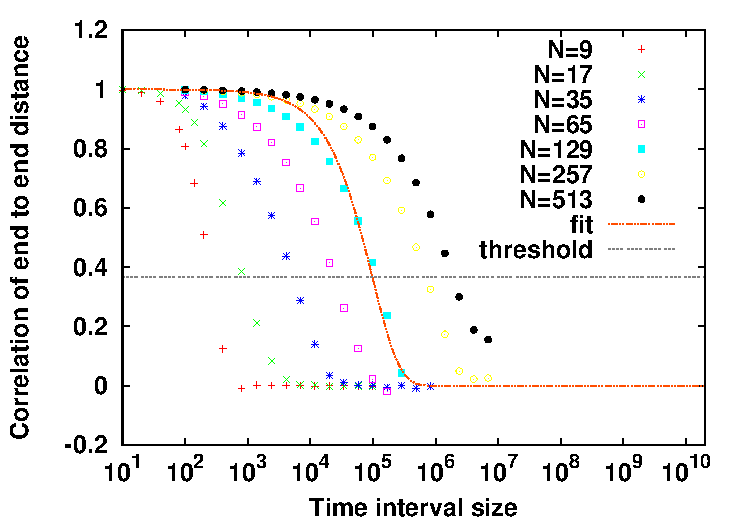
\includegraphics[width=0.9\textwidth]{correlendtoend.pdf}
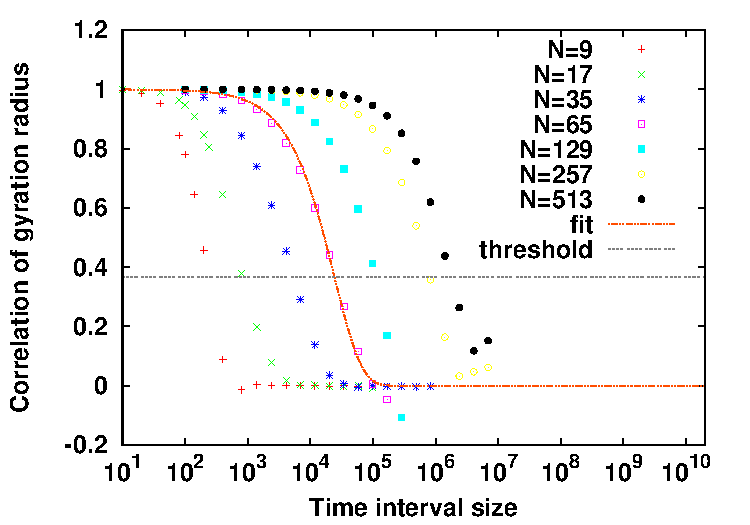
\includegraphics[width=0.9\textwidth]{correlgyr.pdf}

\caption[Résultats numériques: estimation des temps de corrélation]{Auto-corrélation associées à la distance bout-à-bout et au rayon de giration pour différentes longueurs de chaîne du polymère structuré. Le fit exponentiel n'est pas toujours parfait, mais il donne une bonne estimation du temps de corrélation.}
\label{correl}
\end{center}
\end{figure}

\begin{figure}[H]
\begin{center}
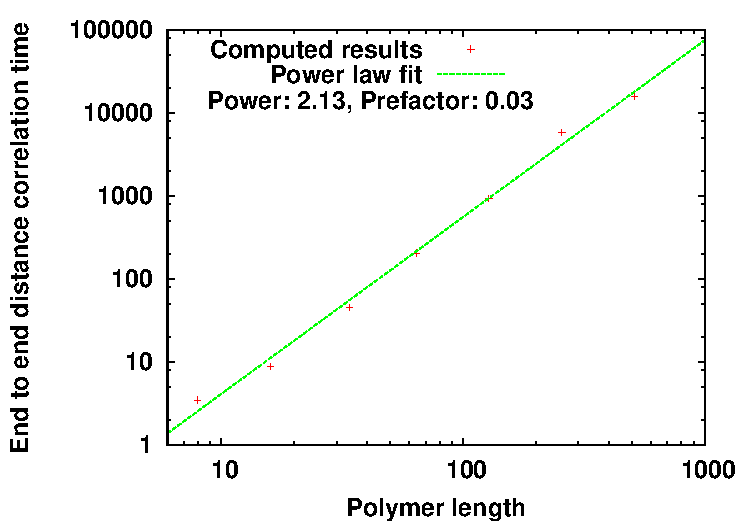
\includegraphics[width=0.9\textwidth]{tpscorrelendtoend.pdf}

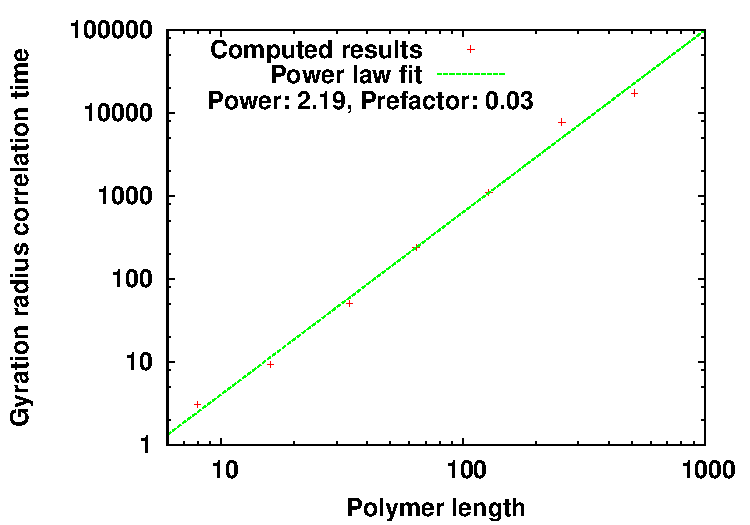
\includegraphics[width=0.9\textwidth]{tpscorrelgyr.pdf}

\caption[Résultats numériques: évolution des temps de corrélation]{En haut: évolution du temps de corrélation de la distance bout-à-bout du polymère. En bas: évolution du temps de corrélation du rayon de giration du polymère. Les valeurs numériques sont très proches de la valeur théorique $\tau_c \propto N^{1+2\nu}$ soit environ $N^{2.176}$. Les effets de taille finie limitent les configurations accessibles et augmente l'exposant de Flory statique $\nu_{static}$, par contre ils ne contraignent pas les fluctuations et les temps nécessaires aux transitions entre configuration, on a donc $\nu_{dynamic}$ bien plus proche de la valeur théorique.}
\label{dyntpscorrel}
\end{center}
\end{figure}


Dans l'étude de la dynamique de notre polymère, nous nous sommes également intéressés au coefficient de diffusion D et à son évolution avec la taille du polymère.

\begin{eqnarray}
\left<(\textbf{r}_{CM}(t)-\textbf{r}_{CM}(0))^2\right>= 6 D_R t
\label{defd}
\end{eqnarray}

Comme le rappel l'équation \ref{defd}, le coefficient de diffusion est lié au déplacement carré moyen du centre de masse. Il ne s'agit pas d'une fonction qui s'évalue à un instant t mais d'une fonction qui s'évalue sur un intervalle de temps. La fonction d’auto-corrélation que nous avons défini précédemment ne peut donc pas être utilisée ici. Nous avons alors fait varier l'intervalle de temps utilisé pour estimer D. On obtient la figure \ref{dexptime}. On remarque que la valeur ainsi évaluée atteint exponentiellement sa valeur réelle de plateau. Le temps caractéristique pour atteindre ce plateau ne dépend pas de la taille de notre polymère. Ce temps ne dépend en effet que d'efforts extérieurs browniens dus à la température. La figure \ref{fluctu-dissip} montre, en accord avec la théorie que D varie bien de manière inversement proportionnelle à la longueur du polymère.

\begin{figure}[H]
\begin{center}
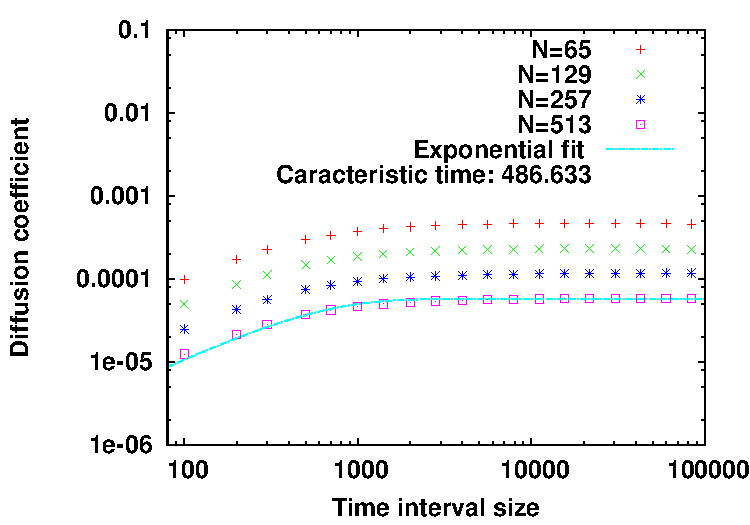
\includegraphics[width=0.8\textwidth]{dexptime.pdf}

\caption[Résultats numériques: estimation du coefficient de diffusion]{Le coefficient de diffusion $D$ est caractéristique de la distance au carrée moyenne parcourue par le centre de masse en un temps $\Delta t$ : $\left<r^2\right> =D\cdot \Delta t$. Nous avons évalué différentes valeurs de $D$ à l'aide de fenêtres glissantes de tailles $\Delta t$ différentes. Pour les petites fenêtres, la valeur de $D$ est fortement sous évaluée. Nous avons remarqué qu'un fit exponentiel de type $D\left(1-\exp\left(-t/\tau\right)\right)$ fonctionne bien et donne quasiment la même valeur de $\tau$ quelque soit le nombre de monomères. $D$ est une caractéristique du centre de masse, il est normal que son amplitude varie avec $N$ car le frottement fluide total évolue avec $N$, et que $\tau$ reste inchangé car il résulte d’efforts extérieurs. Nous avons choisi une fenêtre de taille $5\cdot \tau$ pour évaluer $\left<D(N)\right> $.}
\label{dexptime}
\end{center}
\end{figure}

\newpage

\begin{figure}[H]
\begin{center}
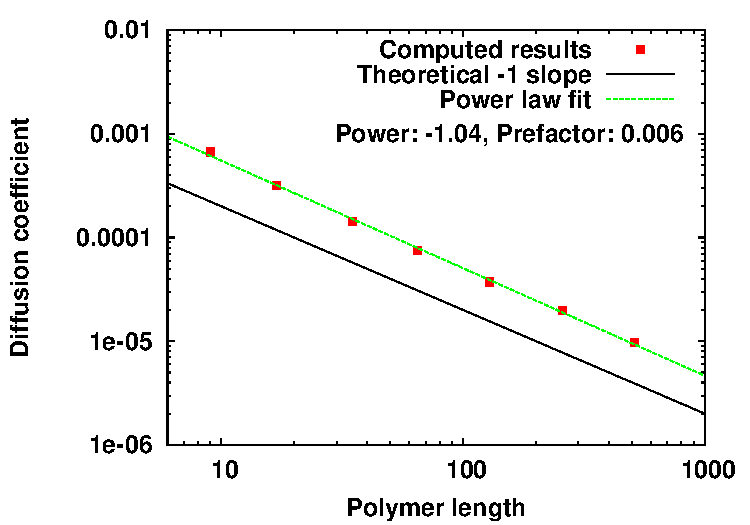
\includegraphics[width=0.9\textwidth]{diffusioncoefficient.pdf}

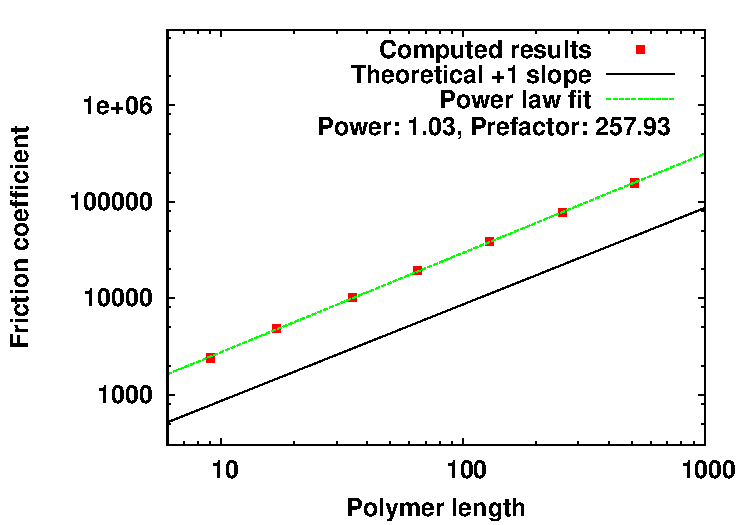
\includegraphics[width=0.9\textwidth]{penteforce.pdf}

\caption[Résultats numériques: évolution des coefficients de diffusion et de friction]{En haut: Décroissance inverse du coefficient de diffusion avec la taille du polymère. En bas: Evolution linéaire du coefficient de friction total avec la taille du polymère.  Le produit des pré-facteurs (1.548 $\epsilon$) donne une bonne estimation de la température du système (défini à 1.5 $\epsilon$). Le théorème de fluctuation-dissipation est ainsi bel et bien vérifié. }
\label{fluctu-dissip}
\end{center}
\end{figure}



Reste maintenant à vérifier le théorème de fluctuation dissipation. Pour cela nous avons imposé une force à une des extrémités du polymère. On observe alors un déplacement linéaire du centre de masse (voir figure \ref{linfrot}). La pente de ce déplacement est calculée pour estimer le coefficient de frottement total du polymère. L'évolution du coefficient de frottement est linéaire. Cette linéarité est attendue car le frottement total est la somme du frottement sur chaque grain. Comme l'illustre la figure \ref{fluctu-dissip}, le calcul de la valeur de ce coefficient de frottement et du coefficient de diffusion sont en accord avec le théorème de fluctuation dissipation.

\begin{figure}[H]
\begin{center}
\includegraphics[width=0.8\textwidth]{traction.pdf}

\caption[Résultats numériques: centre de masse en traction]{Evolution de la position, le long de l'axe de traction du centre de masse pour un polymère de longueur N=129. Le centre de masse évolue linéairement dans l'axe de la force imposée à une extrémité du polymère. Cette évolution linéaire permet d'estimer un coefficient de frottement fluide global pour notre polymère.}
\label{linfrot}
\end{center}
\end{figure}


\subsection{Traction du polymère}

Afin de vérifier le théorème de fluctuation dissipation, nous avons imposé une traction à notre polymère. Par la suite, au cours de nos simulations de translocation, le polymère sera également tracté à travers le pore. Il nous a donc semblé intéressant d'exploiter les données ainsi créées.

\subsubsection{Théorie}

En restant dans le cadre du modèle théorique présenté dans la partie précédente, rappelons l'équation du mouvement régissant note polymère:

\begin{eqnarray}
\large{
\frac{d \textbf{r}(n,t)}{dt} =  \frac{3k_BT}{\nu b^2}\frac{\partial ^2 \textbf{r}(n,t)}{\partial  n^2} + \textbf{g}(n,t)}
\end{eqnarray}

Introduisons maintenant une force en bout de chaîne comme le suggèrent Sakaue et al. \cite{Sakaue2012}:

\begin{eqnarray}
\large{
\frac{d \textbf{r}(n,t)}{dt} =  \frac{3k_BT}{\nu b^2}\frac{\partial ^2 \textbf{r}(n,t)}{\partial  n^2} + \textbf{g}_n} + \frac{\textbf{f}(n,t)}{\nu}
\label{equmvt}
\end{eqnarray}

\begin{eqnarray}
\textbf{f}(n,t) = 2f\delta(n)\cdot\textbf{e}_{y} \text{, tel que} \int_{0}^{N} \textbf{f}(n,t) dn = f \cdot \textbf{e}_{y} 
\end{eqnarray}

On a donc une force f appliquée au monomère $n=0$. Par définition, la position du centre de masse peut s'écrire: 

\begin{eqnarray}
\mathbf{r}_{CM}(t) = \frac{1}{N}\int_{0}^{N} \textbf{r}(n,t) dn
\end{eqnarray}

Et sa vitesse s'obtient en dérivant cette expression et en substituant l'équation \ref{equmvt} dans l'intégrale:


\begin{eqnarray}
\textbf{V} = \left<\mathbf{\dot{r}}_{CM}(t)\right> = \frac{f \cdot \textbf{e}_{y}}{N\nu} 
\label{linearfriction}
\end{eqnarray}
Cette équation \ref{linearfriction} justifie la relation linéaire dont nous parlions précédemment (voir figure \ref{traction}).

La déformation de la chaîne peut être calculée en étudiant les modes normaux déjà définis précédemment. On peut déduire la relation suivante:


\begin{eqnarray}
\left<\mathbf{r}(n,t)-\mathbf{r}_{CM}(t)\right> = \frac{Nb^2f}{k_BT}\left[\frac{1}{9}-\frac{1}{3}\left(\frac{n}{N}\right)+\frac{1}{6}\left(\frac{n}{N}\right)^2\right] 
\label{distmonom}
\end{eqnarray}

Et par conséquence pour $L$, l'élongation de la chaîne: 

\begin{eqnarray}
L=|\left<\mathbf{r}(0,t)-\mathbf{r}(N,t)\right> | = \frac{Nb^2f}{6k_BT} 
\end{eqnarray}

On peut également déterminer la propagation de la tension le long de la chaîne du polymère:

\begin{eqnarray}
T(n) = -\frac{3k_BT}{\nu b^2}\left<\frac{\partial  \textbf{r}(n,t)}{\partial  n}\right> \cdot \textbf{e}_{y} = f \left(1-\frac{n}{N}\right)
\end{eqnarray}

$T(n)$ peut être reliée à la taille moyenne $\xi(n)$ du "blob" \cite{Pincus1976} formé en $n$ (voir figure \ref{sakauetraction}):

\begin{eqnarray}
\xi(n) \simeq \frac{3k_BT}{T(n)}
\end{eqnarray}


Bien entendu, ce modèle ne prend pas en compte l'extension maximale finie des liaisons du polymère, il n'a une certaine validité que pour les faibles forces. A forte force, la distance entre monomères atteint l'extension maximale en début de chaîne.

Regardons la taille de la première liaison en utilisant l'équation \ref{distmonom}:

\begin{eqnarray}
\left<|\mathbf{r}(1,t)-\mathbf{r}(0,t)|\right> = \frac{Nb^2f}{3k_BT} \left(\frac{1}{N}-\frac{1}{2N^2} \right) \underset{N\to+\infty}{\longrightarrow} \frac{b^2f}{3k_BT}
\end{eqnarray} 

On remarque que pour une force critique $f_c$, l'extension maximale $b$ est atteinte.

\begin{eqnarray}
f_c=\frac{3k_BT}{b} 
\end{eqnarray} 

Le modèle décris précédemment n'est plus valable dès que $f$ dépasse $f_c$. Considérons la chaîne étirées sur $m$ segments depuis le point d'application de la force, on a alors une extension jusqu'au monomère m où la tension est égale à $f_c$. Pour les $N-m$ segments restants, le modèle précédent demeure pertinent.
L'extension totale est alors la somme des deux segments:

\begin{eqnarray}
L=  m b + \frac{(N-m)b^2f_c}{6k_BT} = mb + \frac{(N-m)b}{2} = \frac{(N+m)b}{2}
\end{eqnarray}

Il est alors possible de relier $m$ à $f_c$ et de déterminer L:
\begin{eqnarray}
f=  N\nu V = f_c + m\nu V \rightarrow m= \frac{f-f_c}{\nu V} = N\left(1-\frac{3k_BT}{fb}\right)
\end{eqnarray}
\begin{eqnarray}
L= Nb\left(1-\frac{3k_BT}{2
fb}\right)
\label{fc}
\end{eqnarray}



\begin{figure}[H]
\begin{center}
\includegraphics[width=0.6\textwidth]{sakauetraction.jpg}
\caption[Traction d'un polymère]{Modèle simple de l'élongation d'un polymère en traction dans un solvant basé sur un polymère suivant la dynamique de Rouse proposé par Sakaue et al.\cite{Sakaue2012}. En dessous d'une certaine force $f_c$, on observe une légère perturbation de la marche aléatoire du polymère (figure du haut). Le polymère est alors une succession de "blobs" dont la taille dépend de la tension. Lorsque la force de traction est élevée, la chaîne est étirée au maximum jusqu'à ce que la tension retombe à la valeur $f_c$ (en bas).}
\label{sakauetraction}
\end{center}
\end{figure}

Ces résultats théoriques sont valables pour un polymère idéal. Dans notre cas, avec des volumes exclus. Sakaue et al. \cite{Sakaue2012} ne proposent plus de résolution analytique, mais uniquement des raisonnement basés sur des lois d'échelles à faible force (à forte force, les volumes exclus n'interviennent plus sur un polymère étiré).

\subsubsection{Résultats numériques}

Lors de l'évaluation du coefficient de friction de notre polymère, nous l'avons tracté avec une force donnée en bout de chaîne. Précédemment pendant l'évolution du polymère libre, nous avions évalué sa distance bout-à-bout en analysant les coordonnées des monomères de tête et de queues. Ces coordonnées sont maintenant exploitées dans le cas de la traction. 


\begin{figure}[H]
\begin{center}
\includegraphics[width=0.5\textwidth]{xdistribution35.pdf}\includegraphics[width=0.5\textwidth]{xdistribution129.pdf}\\
\includegraphics[width=0.5\textwidth]{ydistribution35.pdf}\includegraphics[width=0.5\textwidth]{ydistribution129.pdf}

\caption[Résultats numériques: distributions pendant la traction]{Distribution des composantes perpendiculaires et parallèles à la force de traction de la distance bout-à-bout de notre polymère. Lorsque la chaîne est tractée à forte force (ici dans la direction y), elle s'étire. On voit comme conséquence de cet étirement que selon la coordonnée x (x queue - x tête),  les effets de volumes exclus de la SAW n'interviennent plus. Les distributions perpendiculaires à la force appliquée retrouvent une distribution gaussienne. Cependant la largeur de cette distribution dépend de la force de traction ; plus on tire fort, plus la queue est rabattue vers le centre. En ce qui concerne la direction y, on constate qu'il existe une distribution également gaussienne qui est de plus en plus éloignée de la tête et de plus en plus resserrée au fur et à mesure que la force augmente. }
\label{traction}
\end{center}
\end{figure}

Pour des forces faibles, on observe des distributions qui ne sont pas gaussiennes car les effets des volumes exclus sont importants sur le polymère qui peut se replier car la traction n'efface pas la diffusion. Pour des forces de traction plus élevées, le polymère est étiré et on a alors des distributions qui redeviennent gaussiennes comme le montre la figure \ref{traction}.


L'élongation de notre polymère a été évaluée grâce aux moyennes de la distribution (y queue - y tête) présentées sur la figure \ref{traction}. Cette élongation est comparée au model théorique simple proposé précédemment dans la figure \ref{elongtraction}. Les résultats obtenus sont satisfaisants, car il n'y a pas de paramètre ajustable, et permettent de valider notre modèle de polymère lorsqu'il est tracté.


\begin{figure}[H]
\begin{center}
\includegraphics[width=0.9\textwidth]{elongation.pdf}

\caption[Résultats numériques: élongations en traction]{Comparaison de l'extension de notre polymère de taille N=129 en traction avec le modèle simple proposé par Sakaue et al. \cite{Sakaue2012}. A très faible force, on observe une déviation qui est due à la présence de volumes exclus, les grains latéraux ayant tendance à favoriser l'élongation du polymère. A forte force, la comparaison est plus juste, notre extension est légèrement plus élevée, ce qui peut venir de l'utilisation d'un potentiel pour les liaisons présentant une longueur d'équilibre de 1$\sigma$, mais une possibilité d'extension maximale (à force infinie) de 1.5$\sigma$.}
\label{elongtraction}
\end{center}
\end{figure}


Ces prédictions théoriques et résultats numériques semblent être en accord avec les images obtenues expérimentalement lors de la traction d'un ADN marqué par fluorophores \cite{Wirtz1995}.\\

Notre modèle de polymère étant consistant, nous pouvons à présent nous intéresser au problème de la translocation.

\cleardoublepage

\chapter{Translocation avec membrane fixe}
\label{translocmurfixe}
\cleardoublepage
{\Large\textbf{Translocation avec membrane fixe}
}\\

\lettrine[loversize=0.6,lraise=0.1,findent=0.5em,nindent=0em]{D}{}ans ce chapitre, nous discutons dans un premier temps des préliminaires afin d'aborder la translocation. Après avoir défini la membrane et les conditions d'équilibration précédent la translocation, nous présentons les différentes théories de la translocation non biaisée puis de la translocation forcée et terminons sur les distributions de temps de translocation attendues. Dans un second temps, nous testons notre polymère dans le cas simple de la translocation à travers une membrane fixe. Cette deuxième partie permet de comparer polymère linéaire simple et polymère structuré ainsi que pore large et pore étroit. Nous proposons également un modèle théorique permettant d'expliquer les différentes phases de la translocation biaisée par l'application d'une force en bout de chaîne et de déterminer le temps de translocation.\\

\minitoc

\begin{center}
\includegraphics[width=0.7\textwidth]{confinit.jpg}
\end{center}



\cleardoublepage








\section{Préparation à la translocation}

\subsection{Définition de la membrane}

Bien que d'autres cristaux bidimensionnels existent, le graphène reste le candidat principal pour le séquençage en utilisant des nanopores dans des membranes fines. Nous avons donc considéré un modèle de membrane proche de ce dernier.
Afin de modéliser la membrane à travers laquelle notre polymère va effectuer une translocation, nous avons choisi de respecter les dimensions relatives  entre le graphène et l'ADN. Un réseau hexagonal de paramètre de maille $\frac{\sigma}{2}$ a été généré (voir figure \ref{reseau}). Le plan de graphène est suffisamment étendu pour qu'avec des conditions aux limites périodiques (pour simuler un plan infini), le polymère le plus grand utilisé ne puisse jamais se retoucher lui même, soit 5488 grains. Cette étendue importante implique que les atomes de notre membrane seront les atomes majoritaires.

\begin{figure}[H]
\begin{center}
\includegraphics[width=0.65\textwidth]{lattice.pdf} 

\caption{Réseau héxagonal constituant la membrane}
\label{reseau}
\end{center}
\end{figure}

Le réseau est ensuite amputé en son centre de tous les grains situés dans un rayon fixé pour créer le pore. Dans ce chapitre, les grains de la membrane sont fixes, les équations du mouvement ne sont pas intégrées pour la membrane, elle n'existe qu'à travers l’Interaction avec le polymère par des potentiels stériques de type Lennard-Jones. Afin d'éviter que le polymère ne pénètre entre les grains de notre membrane, nous avons choisi $\sigma_{ij}=\sigma$ pour toute interaction avec un grain de la chaîne du polymère et $\sigma_{ij}=1.25\sigma$ pour un grain latéral. Cette valeur est supérieur à l'espacement entre grains de la membrane. Physiquement, dans le cas du graphène ces tailles correspondent à la taille des orbitales atomiques de type $\pi$ du graphène avec lesquelles le polymère interagit.


\subsection{Polymère greffé et configurations initiales}

Dans un premier temps, rappelons comme nous l'avons décrit dans le \hyperref[intro]{chapitre 1} que la translocation peut se dérouler dans différents contextes. Elle peut être due uniquement aux fluctuations thermiques, on parle alors de translocation non biaisée, ou être pilotée par une force extérieure, on parle alors de translocation forcée (driven translocation). Les forces extérieures peuvent être de natures variées, on citera notamment l'utilisation de champs électriques (électro- phorèse), de gradients de potentiels chimiques, de flux imposé sur le solvant, ou encore l'emploi de pinces (optiques ou magnétiques) \cite{keyser}. Nous avons choisis de nous placer dans ce dernier cas, notre polymère est donc tracté par une de ses extrémités. En effet, l'alternative plus courante d'appliquer une force au centre du pore (ce qui représente un gradient de potentiel chimique ou électrique) impose de définir une zone d'application de la force qui est clairement définie dans les modèles simples, mais qui deviendrait vite compliquée dans les cas de déformation de la membrane, comme nous l'envisagerons au \hyperref[chapitrememflex]{chapitre 4}. Puisque nous souhaitons que les conditions soient comparables, nous opterons pour la traction de notre polymère en bout de chaîne.



Nous avons dans le \hyperref[intro]{chapitre 1} parlé d'une barrière d'énergie à franchir pour effectuer la translocation d'un polymère, calculons la. Pour cela, nous devons dans un premier temps détermi- ner la probabilité de distribution d'un polymère idéal greffé à une paroi. La chaîne idéale présente comme conditions aux limites, la non pénétration des monomères à travers la paroi. On note $P(\textbf{r},\textbf{r}_0,n)$ la probabilité de trouver le $n$-ième monomère en position $\textbf{r}$, pour $n \gg 1$, le premier monomère étant greffé en $\textbf{r}_0$. $P_0$ est la distribution calculée dans le \hyperref[eqdif]{chapitre précédent} pour un polymère idéal libre:

\begin{eqnarray}
P_0(\textbf{r},\textbf{r}_0,n)=\left(\frac{3}{2\pi n b^2}\right)^\frac{3}{2}\exp\left(-\frac{3(\textbf{r}-\textbf{r}_0)^2}{2 n b^2}\right)
\end{eqnarray}

A l'instar de nombreux problèmes d'électromagnétisme ou de mécanique des fluides, on utilise la méthode des images miroirs afin de déterminer $P(\textbf{r},\textbf{r}_0,n)$. En effet, on a:

\begin{eqnarray}
P(\textbf{r},\textbf{r}_0,n) \propto P_0(\textbf{r},\textbf{r}_0,n)-P_0(\textbf{r},-\textbf{r}_0,n)
\end{eqnarray}

La membrane joue alors le rôle de miroir plan (analogie optique \cite{lipson2011optical}), de conducteur (analogie électrostatique \cite{jackson1999classical}) ou encore d'obstacle sur lequel rebondi un jet (source miroir en mécanique des fluides \cite{kundu2008fluid}).

Dans le cas idéal, la probabilité de distribution du monomère de queue est à variables séparables. En posant $\textbf{r}_0= \epsilon y$ avec $\epsilon \ll 1$, un développement limité au premier ordre donne:

\begin{eqnarray}
P(\textbf{r},\textbf{r}_0,n) \propto \left(\frac{3}{2\pi n b^2}\right)^\frac{3}{2} \left(\frac{6 y \epsilon}{n b^2}\right)\exp\left(-\frac{3\textbf{r}^2}{2 n b^2}\right)
\end{eqnarray}

Cette probabilité est à variables séparables, c'est à dire qu'elle peut s'écrire comme le produit d'une fonction de x, d'une fonction de y  et d'une fonction de z. Selon x et z (la membrane occupant le plan y=0), la distribution reste inchangée (et donc gaussienne) par rapport au cas du polymère libre, il n'y a une influence sur les configurations interdites par la membrane que selon l'axe y. Pour le cas d'un polymère non idéal, les termes supplémentaires introduits dans $P_0$ ne permettent pas de séparer les variables et d'obtenir une expression analytique. Cependant l'allure de la distribution du monomère de queue reste proche du cas idéal tout en présentant des caractéristiques dues aux volumes exclus (voir figure \ref{polagainstwall}). Afin d'aborder la translocation, nous avons dû créer des configurations indépendantes de polymères à l'équilibre, juste avant l'application d'une force. Lors de ce processus de génération, nous avons laissé le polymère évoluer librement en fixant une extrémité au centre du pore. Les 1000 configurations initiales sont toutes séparées d'au moins dix temps de corrélation du polymère afin de garantir qu'elles soient statistiquement indépendantes.


\begin{figure}[H]
\begin{center}


\includegraphics[width=0.7\textwidth]{confinit.jpg}
\includegraphics[width=0.9\textwidth]{probdistribution.pdf}


\caption[Polymère greffé sur une membrane]{En haut: Capture d'écran de la visualisation avec VMD \cite{HUMP96,STON2001} d'une configuration de notre polymère structuré évoluant avec une extrémité fixée au centre du nano-pore. En bas, probabilité de distribution théorique du monomère de queue pour un polymère idéal et résultats numériques pour notre polymère (N=35 grains latéraux). Parallèlement à la membrane, la distribution gaussienne idéale est aplatie au centre à cause de la zone d'exclusion des autres monomères. De même pour la direction perpendiculaire, le pic maximum est repoussé par la présence d'autres monomères. Dans les deux cas, l'éloignement maximal n'est pas modifié car le cas idéal correspond déjà à des chaînes étirées sans superposition de monomères. }
\label{polagainstwall}
\end{center}
\end{figure}

\section{Théories de la translocation}

\subsection{Théories de la translocation non biaisée}


La probabilité de distribution du polymère accolé à une membrane permet, à partir de la fonction de partition stérique, $Z_S(n)= \int_{y>0} P(\textbf{r},\textbf{r}_0,n) \textbf{dr}$, de calculer l'énergie libre d'origine entropique d'un tel système. Dans la limite $n \gg 1$, le premier terme non nul du développement limité impose la loi d'échelle: $Z_S(n) \propto n^{\gamma'-1}$ (on aura un facteur $\gamma'$=1/2 pour un polymère gaussien, 0.68 pour un polymère avec volumes exclus,  ($\nu$=0.588) ou 1 pour une chaîne rigide). Pour un polymère idéal de $N$ monomères en cours de translocation, lors du passage du $n$-ième monomère, Sung et Park \cite{Sung1996} décrivirent les premiers la valeur de l'énergie libre en prenant en compte les effets entropiques de part et d'autre de la membrane:
\begin{eqnarray}
F(N,n)= -k_BT\ln\left(Z_S(n)Z_S(N-n)\right)= \frac{1}{2} k_BT \ln \left(n(N-n)\right) +cste
\label{energbar}
\end{eqnarray}

Cette barrière d'énergie à franchir au cours de la translocation peut être altérée en appliquant une différence de potentiel, chimique ou électrique, ou encore en appliquant directement une force sur la chaîne. La Figure \ref{energiebarrier} montre cette barrière d'énergie.
 Dans le cas d'un polymère non idéal avec volumes exclus, Muthukumar \cite{Muthukumar1999} a montré que l'équation du polymère idéal \ref{energbar} était une simplification de l'équation suivante plus générale:

\begin{eqnarray}
\frac{F(N,n)}{k_BT}= (1-\gamma_2')\ln(n)+ (1-\gamma_1')\ln(N-n)+cste
\label{energbarsaw}
\end{eqnarray}

avec $\gamma_i'$ l'exposant caractéristique de la taille du polymère dans le milieu i ($\gamma_i'$=0.5 pour un polymère idéal ou un milieu saturé en polymère,$\gamma_i'$=0.68  pour un polymère avec volumes exclus ($\nu$=0.588) ou encore 1 pour des polymères ultra rigides ou rod-like en anglais).

Dans le cas général, $\gamma_1'$=$\gamma_2'$ et la translocation est biaisée par une différence de potentiel (chimique, électrique...), on alors la relation:

\begin{eqnarray}
F(N,n)= -k_BT(1-\gamma')\ln \left(n(N-n)\right) + n \Delta \mu +cste
\label{energbargen}
\end{eqnarray}

Dans notre cas, nous n'avons pas une différence d'énergie qui s'applique à la barrière entropique, mais la contribution du travail d'une force (sa transmission le long de la chaîne sera discutée avec les résultats).

Sung, Park et Muthukumar \cite{Sung1996,Muthukumar1999} utilisent cette énergie pour résoudre l'équation dite de Fokker-Planck qui traite l'évolution de la probabilité d'avoir $n$ monomères qui ont effectué la translocation:
\begin{eqnarray}
\frac{\partial P(n,t)}{\partial t} =   \mathcal{L}_{FP}(n) P(n,t)
\label{equfokkerplank1}
\end{eqnarray}

Avec l'opérateur $\mathcal{L}_{FP}(n)= (1/b^2)(\partial/\partial n) D(n)[\exp(-F(N,n)/k_BT)](\partial/\partial n)[\exp(F(N,n)/k_BT)]$

Chuang, Kantor et Kardar \cite{Chuang2001} notèrent que cette équation, dans le cas non biaisé, peut être réduite à:

\begin{eqnarray}
\frac{\partial P(n,t)}{\partial t} =   \frac{\partial ^2 P(n,t)}{\partial ^2 n} +(1-\gamma') \frac{\partial  }{\partial  n}\left(P(n,t)\frac{1-2n}{(1-n)n}\right)
\label{equfokkerplank2}
\end{eqnarray}
grace aux changements de variable:
$n \rightarrow nN$ et $t \rightarrow tD/N^2$


Gardons à l'esprit que ces équations sont valables dans la mesure où le polymère demeure à l'équilibre thermodynamique au cours de la translocation, hypothèse de travail qui sera remise en cause par la suite.



\begin{figure}[H]
\begin{center}
\includegraphics[width=0.7\textwidth]{transelec.jpg} \includegraphics[width=0.5\textwidth]{transpotchim.jpg}

\caption[Translocation, barrière d'énergie d'origine entropique]{Modification de la barrière entropique par une différence de potentiel électrique (en haut \cite{these}) et de potentiel chimique (en bas \cite{Sung1996}). A: différence de potentiel opposée à la translocation, B: différence de potentiel nulle, C: différence de potentiel favorable.}
\label{energiebarrier}
\end{center}
\end{figure}

L'équation précédente \ref{equfokkerplank2} ne faisant plus apparaître $N$, on peut en déduire qu'il existe un paramètre $\alpha$ universel qui permet de décrire le temps de translocation.
\begin{eqnarray}
\tau \propto N^\alpha
\label{tauunbiased}
\end{eqnarray}


 Reste à déterminer $\alpha$. En utilisant des conditions aux limites appropriées (réfléchissante en 0 pour empêcher le retour du polymère et absorbante en bout de chaîne) la résolution de l'équation de Fokker-Planck donne $\tau \propto N^{2}/D$. Le coefficient de diffusion à utiliser est sujet de discorde, Sung et Park \cite{Sung1996} considèrent le coefficient de diffusion comme étant celui du polymère libre et donc inversement proportionnel à $N$ (\hyperref[fluctudissip]{voir chapitre 2}), ce qui leur fait prédire $\tau \propto N^{3}$, Muthukumar \cite{Muthukumar1999} lui, considère que c'est le coefficient de diffusion du polymère au sein du pore qui est pertinent (D est donc une constante) d'où son affirmation $\tau \propto N^{2}$.
 
  Cependant, ses exposants sont vite remis en question par Chuang, Kantor et Kardar \cite{Chuang2001}. Ils arguent que le temps de translocation ne peut pas être plus court que le temps de relaxation du polymère, proportionnel à $N^{1+2\nu}$(comme nous l'avons vu au \hyperref[fluctudissip]{chapitre 2}), qui est caractéristique d'un déplacement du polymère sur une distance de l'ordre de son rayon de giration (comme si il n'y avait pas de membrane à franchir). Si l'exposant associé au temps de translocation est plus faible que le temps de relaxation, cela voudrait dire que la chaîne n'a pas le temps de s'équilibrer au cours de la translocation et donc qu'on ne peut pas appliquer l'équation de Fokker-Planck au système. On a alors un phénomène de translocation sous-diffusif.
  
   Des essais de résolution ont été menés en utilisant une équation de Fokker-Planck fractionnelle \cite{Metzler2003} (qui s'applique dans un cas plus général) et trouvent $\tau \propto N^{2+2\nu-\gamma'}$. Une approche suggère une translocation avec plusieurs échelles de temps représentant l'équilibration des liaisons et la diffusion, on aurait alors $\tau \propto N^{2+\nu}$. Une autre tentative d'approche théorique est à partir de l'équation de Langevin généralisée \cite{Panja2010} et prédit $\tau \propto N^2$ pour un polymère idéal, $\tau \propto N^{2+\nu}$ dans le cas de Rouse et $\tau \propto N^{1+2\nu}$ dans le cas de Zimm (avec interactions hydrodynamiques). Il est intéressant de noter que Luo et al. \cite{2Luo2006} trouvent une évolution de $\alpha=1+2\nu$ à $\alpha=1$ lorsque la longueur du pore augmente.
   
   Les simulations numériques effectuées n'apportent pas de consensus et estiment des exposants compris entre 2.2 et 2.6, suggérant une forte dépendance aux conditions de simulation et une possibilité d'existence de différent régimes en fonction de l'importance de la friction. En effet une transition entre les deux exposants $1+2\nu$ et $2+\nu$ a été reportée \cite{Panja22010}. Le lecteur intéressé pourra trouver un tableau récapitulatif des valeures de $\alpha$ obtenues lors de la translocation non biaisée dans l'article de revue de Palyulin, Ala-Nissila et Metzler \cite{Palyulin2014}.\\

\subsection{Théories de la translocation forcée}

La question de la translocation non biaisée qui ne fait pas consensus n'a pas empêché la communauté scientifique d'aborder le cas de l'introduction d'une force pour faciliter le phénomène. Il vient naturellement à l'esprit que la contribution d'une force appliquée vers le côté trans va favoriser la translocation et on s'attend donc à pouvoir décrire le temps de translocation de la manière suivante, toujours avec un paramètre $\alpha$ caractéristique du nombre de monomères et un nouvel exposant critique $\delta$ pour la force:

\begin{eqnarray}
\tau \propto N^\alpha / f^\delta
\label{taubiased}
\end{eqnarray}

Il est évident que l'amplitude de la force va influer sur la valeur des exposants critiques $\alpha$ et $\delta$. Dans le cas d'une force extrêmement faible, on s'attend à se retrouver dans le cas précédent de la translocation non biaisée avec $\alpha$ compris entre 2.2 et 2.6. En ce qui concerne l'autre extrême, une force très importante, la translocation est entièrement régie par la force (il n'y a plus la moindre influence de la température) et on attend $\tau \propto 1/f$.
 La plupart des études théoriques et numériques se concentrent sur le cas de l'application de la force au sein du pore. Le cas du polymère tracté est plus rarement abordé.
 
 Dans le cas général, l'hypothèse de quasi-équilibre utilisée pour résoudre analytiquement le cas de la translocation non biaisée est maintenant encore moins pertinente avec l'ajout d'une force. Il est par contre toujours possible de définir une limite inférieure à la valeur de $\alpha$. En effet si on considère le cas de l'application d'une force en l'absence de membrane, la translocation est effectuée quand le polymère a franchi une membrane virtuelle, il a donc été déplacé sur une distance de l'ordre de son rayon de giration. Or avec la friction, la vitesse moyenne du centre de masse s'écrit: $v \propto f/N$, d'où $\tau \propto N^{1+\nu}/f$. On envisage donc $\alpha=1+\nu$ comme limite inférieure \cite{Kantor2004}.
 
 Dans le cas d'une force appliquée au sein du pore, cet exposant a été tantôt confirmé tantôt infirmé. Une transition entre exposants allant de $\alpha=2\nu$ à $\alpha=1+\nu$ a vite était observée dans des modèles à deux dimensions \cite{Huopaniemi2006,2Luo2006,Luo2007}. Pour les simulations à 3 dimensions, Luo et al. \cite{Luo2009} suggèrent de distinguer la translocation lente donnant une valeur de $\alpha$ proche de $1+\nu$ trouvée par certains auteurs \cite{Kantor2004,Gauthier2008}, de la translocation rapide donnant une valeur de $\alpha$ plus faible $\alpha \approx 1.4$ \cite{Bhattacharya2009,Luo2008,Sakaue2007} (ce qui va à l'encontre de la limite inférieure proposée). Pour de faibles forces, une équation de Fokker-Planck fractionnelle en prenant en compte des effets de mémoire à longue portée \cite{Metzler2000}, un coefficient $\alpha = 1+ 2\nu - \gamma' = 1.56$ (proche $1+ \nu=1.59$) est proposé par Dubbeldam et al.\cite{Dubbeldam2007}. En utilisant la théorie de la réponse linéaire avec effets de mémoire, Vocks et al.\cite{Vocks2008} s'opposèrent aux explications de Dubbeldam et al. en proposant $\alpha= \frac{1+2\nu}{1+\nu} =1.37$. Luo et al.\cite{Luo2009} ont donc permis, comme l'illustre la figure \ref{slowandfast} de distinguer deux régimes d'application différents pour ces approches avec un phénomène fortement hors équilibre à fortes forces.
 
 
\begin{figure}[H]
\begin{center}
\includegraphics[width=0.9\textwidth]{slowandfasttransloc.jpg}


\caption[Translocations rapides et lentes]{Régimes proposés par Luo et al. de translocations rapides et lentes dépendants de la friction \cite{Luo2009}.}
\label{slowandfast}
\end{center}
\end{figure}

Pour la valeur de $\delta$, à force modérée, la valeur 1 ( $\tau \propto 1/f$) semble faire consensus. En revanche, à fortes forces certains auteurs trouvent un exposant modifié : $\tau \propto 1/f^{0.8}$ pour Luo et al. \cite{Luo2009} ou encore $\tau \propto 1/f^{0.95}$ pour Ikonen et al. \cite{2Ikonen2012}.

 Un tableau (\ref{tableautransloc}) résumé des différentes valeurs obtenues pour $\alpha$ et $\delta$ permet d'y voir un peu plus clairs dans les resultats et théories très variés.



\begin{table}
\setstretch{1.6}
\begin{center}


\begin{tabular}{|c|c|c|c|}
  \hline
  Valeur de $\alpha$ & Valeur de $\delta$ & Méthode & Auteur et référence \\
  \hline
  1 & \_ & 3D MC & Chern \cite{Chern2001}\\
  1 & \_  & Théorie & Lubensky \cite{Lubensky1999} \\
  1 & \_  & Expérience & Meller \cite{Meller2002} \\
  1 & 1  & 3D BD & Tian \cite{Tian2003} \\   
  1.65 $\pm$ 0.08 & \_  & 3D MC & Milchev \cite{Milchev2004} \\
  1+$\nu$, 2 (traction) & 1  & Théorie, 2D MC & Kantor \cite{Kantor2004} \\
  1+$\nu$ & \_  & Théorie & Matsuyama \cite{Matsuyama2004} \\
  1.6 & \_  & 3D MC & Tsuchiya \cite{Tsuchiya2007} \\
  1.46 $\pm$ 0.01 (courts) & \_  & 2D FB & Luo \cite{Luo2006} \\
  1.72 $\pm$ 0.06 (longs) & \_  & 2D FB & Luo \cite{Luo2006} \\
  1.50 $\pm$ 0.01 (courts) & \_  & 2D LD & Huopaniemi \cite{Huopaniemi2006} \\
  1.69 $\pm$ 0.04 (longs) & \_  & 2D LD & Huopaniemi \cite{Huopaniemi2006} \\
   1.40 (courts) & \_  & Expérience & Wanunu \cite{Wanunu2008} \\
  2.28 (longs) & \_  & Expérience & Wanunu \cite{Wanunu2008} \\
  1+2$\nu-\gamma'$ & 1  & 3D MC & Dubbeldam \cite{Dubbeldam2007} \\
  $\approx$1.9 (traction) & 0.94 $\pm$ 0.01  & 2D LD, Théorie & Huopaniemi \cite{Huopaniemi2007} \\
  $\frac{1+2\nu}{1+\nu}\approx1.37$ & 1 & 2D,3D Théorie MC  & Panja, Vocks \cite{Panja22010,Vocks2008} \\
  1.27 & \_  & Expérience & Storm \cite{Storm2005} \\
  1.42 $\pm$ 0.01 & \_  & 3D MD & Luo \cite{Luo2008} \\
  1.36 $\pm$ 0.01 & \_  & 3D LD & Bhattacharya \cite{Bhattacharya2009} \\
 1.36 $\pm$ 0.03 & \_  & 3D LD & Fyta \cite{Fyta2008} \\
 1+$\nu$ (lente) & 1  & 3D LD & Luo \cite{Luo2009} \\
 1.37$\pm$ 0.02 (rapide) & 0.79$\pm$ 0.02  & 3D LD & Luo \cite{Luo2009} \\
 1+$\nu$ & 1  & Théorie & Saito \cite{Saito2012} \\
 1+$\nu$ (lent) & 0.9-1 fortes forces & Théorie & Ikonen \cite{Ikonen2012} \\
 1+$\nu$ (lent) & 0.9-0.95 fortes forces& 3D LD et BD & Ikonen \cite{Ikonen2012} \\
  
  \hline
\end{tabular}
\caption[Valeurs des exposants critiques]{Valeurs des exposants critiques $\alpha$ et $\delta$ trouvées dans la littérature avec différentes méthodes. Courts ou longs fait référence à la taille du polymère. Abréviations: MC: Monte Carlo, FB: Fluctuating
Bond method, LD: Langevin Dynamics, MD: Molecular Dynamics, BD: Brownian Dynamics.}
\label{tableautransloc}
\end{center}
\end{table}
 
 
 En ce qui concerne la compréhension physique du phénomène, dans une série de papiers, Sakaue et al. \cite{Sakaue2007,Sakaue2010,Saito2011,Saito2012,Sakaue2012} 
 affirment que lorsqu'une force est appliquée sur le polymère, elle n'est pas ressentie directement dans tout le polymère. Il y a alors un front de propagation de la tension. Pour la translocation forcée, avec force au sein du pore, ils distinguent quatre régimes (voir figure \ref{regimeprofiles}).
 
 \begin{figure}[H]
\begin{center}
\includegraphics[width=0.8\textwidth]{regimesprofiles.jpg}
\includegraphics[width=0.5\textwidth]{regimedistrib.jpg} 

\caption[Régimes possibles au cours de la translocation]{Régimes proposés par Sakaue \cite{Saito2011}. (a) Régime d'équilibre (EQ) lors des translocation très lentes. (b) Régime trompette (TP): propagation de la tension le long de blob jusqu’au front où le polymère est à l'équilibre . (c) Régime Tige-fleur (SF: Stem-Flower): Une partie du polymère sous tension est étirée. (d) Régime d'étirement fort (SS: Super-Stretched): La totalité du polymère qui ressent la tension est étirée. La frontière entre les régimes (EQ) et (TP) $f_{\#}$ décroit en $N^{-\nu}$. La valeur $f^*$ entre les régimes (TP) et (SF) correspond à $f_c$ que nous avons défini au \hyperref[fc]{chapitre précédent}. La frontière entre (SF) et (SS), $f^{**}$, évolue elle en $N^{\nu}$. }
\label{regimeprofiles}
\end{center}
\end{figure}
 
  Pour une force très faible (régime avec $\alpha$ compris entre $2+\nu$ et $1+2\nu$), le polymère est toujours à l'équilibre et la translocation est lente, Il n'y a pas propagation de la tension le long de la chaîne car les fluctuations thermiques dominent. Pour une force qui augmente, mais qui ne dépasse pas la valeur $f_c$ définie au \hyperref[fc]{chapitre 2} on observe un régime en trompette. Le polymère présente alors des blobs de tensions jusqu'au front de propagation de la tension qui sépare les blobs de la partie toujours à l'équilibre. Ensuite apparaît le régime tige fleur. Pour une force supérieure à $f_c$, une partie du polymère est en extension comme dans le \hyperref[fc]{chapitre 2}, jusqu'à ce que la tension retombe à $f_c$ (partie tige), puis on observe un schéma similaire au régime trompette (partie fleure composée des blobs et de la partie à l'équilibre). A force très importante, s’installe le régime d'étirement fort. Le polymère est composé d'une partie étirée jusqu'au front de propagation et d'une partie à l'équilibre qui n'a pas encore ressenti la force. Sakaue et al.\cite{Saito2011} trouvent alors dans les 3 régimes (TP), (SF) et (SS), $\alpha=1+\nu$ et des valeurs de $\delta$ définies pour chaque régime. Ce modèle est alors utilisé et corrigé par plusieurs travaux \cite{Ambjrnsson2005,2Ambjrnsson2005,Rowghanian2011,Dubbeldam2012}. 
  
  
La continuation la plus pertinente de ces travaux provient de Ikonen et al., qui ont construit la théorie de la propagation de la tension-dynamique brownienne  (Brownian Dynamics-Tension Propagation theory ou BDTP) \cite{Ikonen2012,2Ikonen2012,Ikonen2013}. Leur théorie est basée sur la combinaison de la dynamique brownienne appliquée à la coordonnée de réaction (le nombre de monomères ayant effectué la translocation) avec une description explicite de la propagation du front de tension dans la chaîne qui génère un terme de mémoire dépendant du temps. Cette théorie prédis que $\alpha=1+\nu$ dans les trois régimes (TP, SF et SS) lorsque N tend vers l'infini. En ce qui concerne l'exposant lié à la force, un passage de $\delta \approx 0.9$ à $\delta=1$ pour les fortes forces est prédit \cite{Ikonen2013}.

\begin{figure}[H]
\begin{center}
\includegraphics[width=0.9\textwidth]{bdtpalpha.jpg}

\caption[Evolution de $\alpha$ selon la théorie BDTP]{Evolution du paramètre $\alpha$ en fonction de la friction prévue par la théorie BDTP \cite{Ikonen2013}. Lorsque N tend vers l'infini, la limite est $\alpha=1+\nu$. Les simulations numériques usuelles trouvant des valeurs inférieures n'utilisent pas des valeurs de N suffisamment élevées.}
\label{bdtp}
\end{center}
\end{figure}

L'aspect le plus intéressant de cette théorie est qu'elle permet d'expliquer la large disparité des valeurs de $\alpha$ trouvées dans la littérature. En effet, le terme correctif lié à la propagation de la tension est assez grand et linéaire en N, ce qui explique que même pour des valeurs aussi élevée que $10^5$, $\alpha$ soit sous évalué (voir figure \ref{bdtp}). Ce terme correctif est physiquement en partie du à la phase dite de rétractation de la queue du polymère (voir figure \ref{tailretractation}). Dans leur article de revue, Palyulin, Ala-Nissila et Metzler \cite{Palyulin2014} présentent un tableau de comparaison entre cette théorie et des simulations numériques de plusieurs références. 



\begin{figure}[H]
\begin{center}
\includegraphics[width=0.75\textwidth]{tailretractinpore.jpg}
\includegraphics[width=0.75\textwidth]{tailretractpulling.jpg} 

\caption[Temps d'attente et rétractation de la queue du polymère]{Temps d'attente des monomères et rétractation de la queue du polymère en fin de translocation. Le temps d'attente d'un monomère est le temps moyen qu'il passe au sein du pore. Haut: cas d'une force exercée au sein du pore \cite{2Ikonen2012}. La rupture de la pente correspond à la période de rétractation de la queue du polymère, la tension s'est entièrement propagée au bout du polymère dont la translocation s'accélère. Bas: cas d'un polymère tiré \cite{Huopaniemi2007}. La rupture de pente se fait sur un plateau.}
\label{tailretractation}
\end{center}
\end{figure}

Cependant, leur prévision $\delta=1$ pour les fortes forces semble ne pas être vérifiée dans les simulations de dynamiques moléculaires \cite{2Ikonen2012}. Certains auteurs avancent une explication liée à l'encombrement du pore du côté trans \cite{Palyulin2014}, d'autres privilégient une influence d'une friction trop forte et/ou de liens trop faibles dans les simulations de dynamique moléculaire \cite{2Ikonen2012}. Pour la translocation forcée par une force située au sein du pore, la théorie BDTP est aujourd'hui celle qui semble la plus robuste.\\


En ce qui concerne le cas du polymère tiré par une de ses extrémités, les travaux sont beaucoup moins nombreux \cite{Kantor2004,Grosberg2006,Huopaniemi2007,Panja2008}. Pourtant, l'évolution du temps d'attente moyen des monomères présenté dans la figure \ref{tailretractation} ou la distribution du polymère au cours de la translocation présentée dans la figure \ref{translocshape}, montrent que les deux façons de forcer la translocation ne sont pas équivalentes.


\begin{figure}[H]
\begin{center}
\includegraphics[width=0.49\textwidth]{transshapeintopore.jpg}\includegraphics[width=0.49\textwidth]{shapetractiontransloc.jpg} 

\caption[Force dans le pore et force en bout de chaîne]{Différence entre force dans le pore et force en bout de chaîne. A gauche: Contours de distribution de type champignon du côté trans qui peut être encombré lorsque la force est générée au sein du pore \cite{Dubbeldam2012}. A droite: Configuration typique lorsque la force est exercée à une extrémitésdu polymère, la partie du polymère du côté trans est étirée et ne crée pas d'encombrement \cite{Huopaniemi2007}.}
\label{translocshape}
\end{center}
\end{figure}




Kantor et Kardar les premiers étudièrent ce cas \cite{Kantor2004} et prédirent $\tau \propto N^2/f^{2-\frac{1}{\nu}}$ pour un polymère idéal tracté à force faible (ce qui correspond à $f<f_c$, définie précédemment). Ces valeurs $\alpha=2$ et $\delta=2-\frac{1}{\nu}$ sont des valeurs limites obtenues par analyse d'échelle. Dans le cas d'une absence de membrane, le temps de translocation du polymère correspond à la distance à parcourir sur la vitesse moyenne. La vitesse moyenne est $V \propto f/N$. Pour la distance à parcourir, ils considèrent que le polymère est formé par loi d'échelle d'une succession de blobs comprenant $N_{B} \propto (k_BT/bf)^{-\nu}$ monomères de taille $ R_{B} \propto bN_B^{\nu}\propto k_BT/f$, il y a un nombre de blobs successifs $N/N_B \propto N (fb/k_BT)^{1/\nu}$. La distance à parcourir est  $L \propto R_B(N/N_B) \propto bN(fb/k_BT)^{\frac{1}{\nu}-1} $. On peut alors déduire $\tau \propto \frac{L}{V} \propto N^2/f^{2-\frac{1}{\nu}}$. Nous remettons en cause cette vision avec les travaux de Sakaue \cite{Sakaue2012} vus au \hyperref[fc]{chapitre précédent} qui rebutent l'image de blobs successifs de taille similaire au profit de blobs de taille croissante ; l'élongation $L$ est alors proportionnelle à $Nf$. On a donc plutôt $\tau \propto \frac{L}{V} \propto N^2/f^{2}$. Cette remarque ne modifie pas la valeur limite de $\alpha$ prévue,  de plus la forme trompette ainsi envisagée est incompatible avec le passage au sein du pore qui va limiter la taille des blobs .

 Kantor et Kardar avancent alors que la même valeur de $\alpha$ est attendue dans le cas du modèle de Rouse. Cette affirmation se base sur l'argument suivant: la chaîne est étirée du coté trans (elle ne subie alors aucune influence de volume exclu) et c'est entièrement ce côté qui va piloter la translocation. Ils vérifient alors leurs prédictions par simulation de type Monte-Carlo à 2 dimensions. Pour le polymère idéal, ils trouvent $\alpha =1.936 \pm 0.01$, valeur en augmentation avec la longueur de la chaîne (les effets de tailles finis réduisent la valeur de $\alpha$) et confirment une loi asymptotique de $\alpha=2$. Dans le cas d'un polymère de Rouse, ils trouvent $\alpha =  1.875 \pm 0.005$, également en augmentation et avancent donc un comportement asymptotique de $\alpha=2$. En ce qui concerne la valeur de $\delta$, la figure \ref{deltakantor} montre un comportement asymptotique qui se rapproche de $1/f$. 
% Notre remarque porte sur la valeur de $\delta$, or on s'attend à une transition de $\delta=0$ pour les forces faibles (cas proche de la translocation non biaisée) à une limite asymptotique qui ne peux pas être supérieure à $\delta=1$. La  valeur de 2 que nous proposons ne se situe pas dans cet intervalle [0:1], contrairement à la valeur $\delta=2-\frac{1}{\nu}$.
 %et l'origine ayant un comportement linéaire conforte notre estimation d'exposant $\delta$.
 
 \begin{figure}[H]
\begin{center}
\includegraphics[width=1\textwidth]{kantorkardar.jpg}
\caption[Exposants critiques pour une translocation tractée]{ A forte force, Kantor et Kardar \cite{Kantor2004} trouvent  $\alpha=1.875$ et $\delta=1$. A droite: estimation de $\alpha$. A gauche: graphe réajusté dont le plateau à haute force montre que $\delta=1$.}
\label{deltakantor}
\end{center}
\end{figure}

Ces valeurs sont confirmées par Huopaniemi et al. \cite{Huopaniemi2007}, ainsi que par Panja et Barkema pour la valeur à forte force \cite{Panja2008}. Ces derniers contestent cependant la valeur à faible force qui revient au cas de la translocation non biaisée (notons que ce papier est antérieur à d'autres travaux qu'ils ont réalisé dont nous avons parlé précédemment et qui reportaient une transition entre exposants $1+2\nu$ et $2+\nu$ dans le cas de la translocation non biaisée \cite{Panja22010}).

 Dans leurs travaux, Huopaniemi et al. \cite{Huopaniemi2007} analysent également le cas de la translocation à travers un pore infiniment large. Malgré le fait que l'article correspondant ne détaille pas comment ce pore infiniment large est implémenté ( S'agit-il d'une translocation sans membrane ? Les configurations initiales sont générées contre une membrane puis celle ci disparaît lors de la phase de translocation ? Utilisent-ils un pore très grand devant le rayon de giration du polymère ? Quid de l'hypothèse d'un seul monomère au sein du pore à tout instant ? ), il est intéressant de remarquer qu'ils trouvent un régime unique pour leur pore standard et trois régimes différents pour le pore infiniment large (voir figure \ref{regimestransloctractee}).

\begin{figure}[H]
\begin{center}
\includegraphics[width=1\textwidth]{regimespulling.jpg}
\caption[Régimes de forces pour une translocation tractée]{Translocation forcée en tirant le polymère par une de ses extrémités \cite{Huopaniemi2007}. (a) : translocation à travers un pore infiniment large, trois régimes sont observables. A faible force, la force n'influence pas le temps de translocation, on est alors proches du cas non biaisé. A force intermédiaire, $\delta$ augmente pour correspondre à 2/3, valeur anticipée par la loi d'échelle conduisant à $\delta=2-\frac{1}{\nu}$ pour ces simulations à deux dimensions. A forte force $\delta$ augmente encore pour se rapprocher de 1. (b) : Translocation à travers un pore non infiniment large. Un seul régime demeure avec $\delta$ proche de 1.}
\label{regimestransloctractee}
\end{center}
\end{figure}

Tâchons de comparer les trois régimes observés dans le cas du polymère tiré par une extrémité aux quatre du cas de la translocation biaisée par une différence de potentiel. A notre connaissance, aucun travaux ne porte sur le cas du polymère tracté en prenant en compte le modèle de Sakaue et al. ou la théorie BDTP. Le premier régime correspond dans les deux cas à une force faible et a un phénomène proche de la translocation non biaisée. Les régimes (TP) et (SF) présentés dans le cas de la translocation forcée par différence de potentiel ne sont plus pertinents dans le cas du polymère tiré. En effet la forme de la trompette est incompatible avec le passage à travers le pore. Lorsque le diamètre du col de la trompette est comparable à celui du pore, le mouvement est ralenti et le polymère s'étire du côté trans. On se retrouve alors avec la forme d'un des trois régimes (TP), (SF) ou (SS) du côté trans. avec pour taille de blob maximale des régimes (TP) et (SF), le diamètre du pore. A très forte force, on a l'équivalent du régime (SS) avec un front de propagation de la tension situé soit au niveau du pore, soit qui remonte du côté cis. 


%A force très importante, le polymère est entièrement étiré, on a le régime (SS) du côté cis dans le cas de la différence de potentiel.Pour le polymère tiré, le régime (SS) se situe des deux côtés de la membrane (le polymère est entièrement étiré de part et d'autre de la membrane jusqu'au front de propagation de la tension).

 Ces exposants sont également corroborés à forte forces dans un cas presque similaire, celui de la désorption de polymères \cite{Paturej2012}. En effet le cas d'un polymère attaché à une surface dont on tire une extrémité peut être vu comme le même problème avec une composante d'affinité avec le support d'absorption qui fait office de barrière énergétique à franchir. L'analogie est proche du cas d'un pore étroit ou il faudrait une force seuil pour amorcer la translocation. En ce qui concerne les exposants du cas de la translocation biaisée par une différence de potentiel, une analogie peut être faite avec l'ouverture et de la fermeture d'épingles dans l'ADN ou l'ARN \cite{Ferrantini2011}.


 \newpage

\subsection{Distribution du temps de translocation}

Dans leurs travaux sur la translocation, Daniel Y Ling et Xinsheng Sean Ling \cite{Ling2013} proposent d'étudier la distribution des temps de translocation en considérant la translocation comme un phénomène de diffusion biaisée unidimensionnelle. Ils considèrent le pore suffisamment fin comparé à la longueur du polymère pour être considéré comme un marcheur qui se déplace le long de ce dernier. Ils peuvent donc lui appliquer l'équation de Fokker-Planck:

\begin{eqnarray}
\frac{\partial P(x,t)}{\partial t} =   D\frac{\partial ^2 P(x,t)}{\partial ^2 x} - \nu \frac{\partial  P(x,t)}{\partial  x}
\label{equfokkerplank}
\end{eqnarray}

Avec $P(x,t)$ la probabilité pour le pore d'être à la coordonnée $x$ le long du polymère à l'instant $t$, $D$ le coefficient de diffusion et $\nu$ la vitesse du marcheur. Ils utilisent pour conditions aux limites, le premier monomère au sein du pore à $t=0$ et une absorption lorsque le pore atteint $L$ l'extrémité du polymère, il n'y a pas de retour possible:

\begin{eqnarray}
 P(x,0) =   \delta(x)\text{  }, \text{  } P(L,t)=0
\label{condlim}
\end{eqnarray}

La solution de l'équation différentielle est:

\begin{eqnarray}
 P(x,t) = \frac{1}{\sqrt{4\pi D t}} \left(e^{-\left(x-\nu t\right)^{2}/4Dt} -e^{(\nu L/D)}e^{-\left(x-2L-\nu t\right)^{2}/4Dt} \right)
\label{equfokkerplanksol}
\end{eqnarray}

La distribution du temps de translocation est la distribution du temps de premier passage:

\begin{eqnarray}
 F1(t) = -\frac{d}{dt}\int_{-\infty}^L  P(x,t) dx
\label{firstpassageint}
\end{eqnarray}

\begin{eqnarray}
 F1(t) = \frac{L}{\sqrt{4\pi D t^3}} e^{-\left(L-\nu t\right)^{2}/4Dt}
\label{firstpassage}
\end{eqnarray}

Avec l'équation \ref{firstpassage} ils arrivent à reproduire des résultats expérimentaux dans certaines conditions où la vitesse du marcheur peut être aisément reliée aux conditions expérimentales, les hypothèses $D$ et $\nu$ constants valables. Nous nous servirons de cette équation pour analyser les distributions de nos temps de translocation.





\section{Résultats numériques et théoriques}

Nous avons étudié trois cas différents dans le cadre de notre travail sur une membrane fixe. Dans un premier temps, la translocation d'un polymère non structuré à travers un pore suffisamment large pour limiter les frottements est expérimentée. Nous avons retiré 24 grains du centre de la membrane pour former le nanopore. Puis nous avons testé notre polymère structuré, également dans un pore suffisamment large, il a alors fallut retirer 54 grains. Pour terminer nous avons investigué l'effet d'un nanopore étroit sur la translocation du polymère structuré en retournant à un pore constitué par le retrait de 24 grains. Les deux pores utilisés sont présentés sur la figure \ref{bothpores}.
 \begin{figure}[H]
\begin{center}
\includegraphics[width=0.45\textwidth]{holebigger.pdf} \includegraphics[width=0.45\textwidth]{holesmall.pdf}

\caption[Nanopores utilisés]{Les deux nanopores utilisés. A gauche: Pore large pour la translocation de polymères structurés. A droite: Pore étroit pour la translocation de polymères structurés et larges pour des polymères simples linéaires. Un zoom sur les pores et la taille relative des grains du polymère en cours de translocation seront fournis par la suite  pour chaque expérience.}
\label{bothpores}
\end{center}
\end{figure}

\subsection{Translocation du polymère simple}


Afin d'avoir une base de comparaison, nous avons étudié le cas du polymère linaire simple dont nous avons étudié la translocation à travers un nanopore relativement large (voir figure \ref{porelargesimplepol}). Cette base nous servira aussi bien de vérification par rapport à la littérature existante que d'étalon pour notre polymère structuré.


\begin{figure}[H]
\begin{center}
\includegraphics[width=1\textwidth]{simplepolpore.pdf}


\caption[Polymère simple dans le pore]{Pore large utilisé pour la translocation de notre polymère linéaire simple. Les tailles des différents grains sont respectées. }
\label{porelargesimplepol}
\end{center}
\end{figure}

Les grains de la membrane interagissent avec le polymère avec des potentiels de Lennard-Jones tel que $\sigma_{mp}=1$ soit supérieur au pas du réseau. Nous sommes alors sûrs que le polymère ne peut pas pénétrer la membrane ailleurs qu'au sein du pore.\\

\begin{figure}[H]
\includegraphics[width=0.5\textwidth]{simplepoltransloc1.jpg}\includegraphics[width=0.5\textwidth]{simplepoltransloc2.jpg}
\begin{minipage}{0.5\linewidth}
\includegraphics[width=\textwidth]{simplepoltransloc3.jpg}
\end{minipage}
\begin{minipage}{0.5\linewidth} 
\caption[Capture d'écran de la translocation du polymère simple]{Captures d'écran au cours d'une translocation typique.La partie du côté cis conserve une conformation en pelote, le côté trans est en extension. Cela laisse entrevoir un côté cis à l'équilibre dominé par les fluctuations thermiques et un côté trans dominé par la force exercée à l’extrémité du polymère. Nous reviendrons sur cet aspect lors de l'élaboration d'un cadre théorique pour traiter la translocation d'un polymère tracté.}
\label{screenshotspolsimple}
\end{minipage}
\end{figure}



\noindent Après avoir généré les 1000 configurations d'équilibre, nous tentons d'effectuer 1000 translocations sur une plage de valeurs de force comprises entre 0.1 et 100 unité de Lennard Jones. Nous avons étudié 3 polymères de taille 16, 32 et 64 grains, un quatrième de 128 grains est partiellement étudié afin d'estimer des valeurs de $\alpha$ sur plus de trois points. Une translocation typique est montrée sur la figure \ref{screenshotspolsimple} et la figure \ref{taupolsimple} présente les résultats que nous avons obtenus.
 
\begin{figure}[H]
\begin{center}
\includegraphics[width=0.9\textwidth]{translocpolsimple.pdf} 
\caption[Temps de translocations du polymère simple]{Temps de translocation moyen du polymère en fonction de la force de traction exercée. A faible forces, un plateau semble indiquer  que nous nous situons dans le régime proche de la translocation non biaisée. Lorsque la force est plus importante, la valeur moyenne du temps de translocation décroit d'une manière qui semble proportionnelle à l'inverse de la force exercée.}
\label{taupolsimple}
\end{center}
\end{figure}

On peut clairement distinguer un plateau à faibles forces et une rupture de pente suivie de la décroissance du temps de translocation lorsque la force augmente. A l'aide de ses données brutes, tâchons d'estimer les valeurs de $\alpha$ et $\delta$. Pour $f<1$ nous sommes sur le plateau et nous estimons $\alpha=2.01 \pm 0.05$ pour $f=0.5$. Pour $f>1$, notre estimation est $\alpha=1.84 \pm 0.01$ pour $f=30$. La figure \ref{ndeppolsimple} présente les valeurs de $\alpha$ trouvées dans ces deux régimes. Ces résultats sont inférieurs aux valeurs théoriques prévues car nous avons des polymères relativement courts.

\newpage


\begin{figure}[H]
\begin{center}
\includegraphics[width=0.9\textwidth]{ndeppolsimplef05.pdf}
\includegraphics[width=0.9\textwidth]{ndeppolsimplef30.pdf}

\caption[Temps de translocations en fonction de N]{Evolution du temps de translocation moyen avec N. En haut, pour une faible force, nous estimons $\alpha=2.01 \pm 0.05 $ (la valeur pour N=128 étant réalisée sur une translocation unique, elle n'a pas été prise en compte dans le calcul de $\alpha$), pour une valeur théorique attendue $\alpha=1+2\nu \approx 2.18$ pour une translocation non biaisée. En bas, pour une force modérée, $\alpha= 1.84 \pm 0.01$, pour une valeur théorique attendue de 2. Nos valeurs de $\alpha$ sont sous estimées à cause d'effets de taille finie car nos polymères sont courts.}
\label{ndeppolsimple}
\end{center}
\end{figure}

\newpage


Afin de visualiser les différents régimes, nous avons retracé les temps de translocation de manière réajustée. Connaissant $\alpha$ dans le régime décroissant et soupçonnant une valeur de $\delta$ proche de 1, nous avons retracé $\tau \cdot f/N^{\alpha}$ (avec $\alpha=1.84$). Les résultats obtenus sont présentés sur la figure \ref{simplepolrescale}.


\begin{figure}[H]
\begin{center}
\includegraphics[width=0.9\textwidth]{transloctaufsimplepolresc.pdf}


\caption[Temps de translocations réajustés]{Temps de translocation réajusté en fonction de la force exercée. La force réduite correspond à la division de l'échelle d'énergie donnée par la force par celle donnée par la température. On observe clairement une rupture de pente qui traduit le changement de régime entre translocation non biaisée et translocation forcée. Lorsque la force est intermédiaire, $\delta=1$, comme attendu, cependant à forte force, on observe une diminution de $\delta$, avec $\tau \propto f^{-0.82}$.}
\label{simplepolrescale}
\end{center}
\end{figure}

Ce réajustement des temps de translocation permet d'observer, à forte force, une diminution de $\delta$ qui sature à 0.822 $\pm$ 0.006 . Nous avons vu que dans la littérature, ce comportement apparaît aussi bien dans le cas de la translocation forcée par différence de potentiel que dans le cas de la force de traction à une extrémité. Cette situation semble éliminer l'explication avancée concernant un effet d'encombrement dû au polymère du côté trans \cite{Palyulin2014}. Nous nous proposons de tester l'hypothèse de liaisons et/ou friction du solvant trop faible/forte \cite{2Ikonen2012}. 

Nous nous sommes placés dans un cas simple, déterministe, aisément soluble numériquement. Le polymère est placé perpendiculairement à la membrane avec le premier monomère au milieu du pore. La température est nulle, nous faisons varier $\nu$, le coefficient de frottement des grains avec le solvant et $k$, la constante de raideur associée aux liaisons entre grains. Les résultats que nous obtenons, présentés dans le tableau ci-dessous, permettent d'accréditer l'hypothèse de liaisons et/ou friction trop faible/forte.

\begin{table}[H]
\begin{center}
\setstretch{1.2}
\begin{tabular}{|c|c|c|}
  \hline
  Valeur de $\nu$ & Valeur de $k$ & Valeur de $\delta$ \\
  \hline
  0.1 & 30 & 0.989 $\pm$ 0.007\\
  0.33 & \_  & 0.972 $\pm$ 0.004 \\
  1 & \_ & 0.884 $\pm$ 0.05  \\
  3 & \_  &  0.62 $\pm$ 0.02  \\
  10 & \_  &  0.51 $\pm$ 0.02 \\
  30 & \_  &  0.478 $\pm$ 0.02  \\
  1 & 3  &  0.85 $\pm$ 0.02  \\
  1 & 300  &  0.90 $\pm$ 0.02\\
  \hline
 
    
\end{tabular}
\caption[Influence de la friction et de la force des liaisons sur le comportement à forte force]{Valeurs de $\delta$ trouvées à fortes forces pour différents paramètres de friction et de force de liaison en supprimant le bruit thermique. Simulations déterministes réalisées sur un polymère composé de 16 grains alignés à l'équilibre perpendiculairement à la membrane, le premier grain sur lequel s'applique la force situé au centre du pore. Ces valeurs permettent d'expliquer les valeurs de $\delta$ inférieure à 1 à fortes forces.}  

\end{center}

\end{table}

Cette hypothèse semble validée, dans le cas où il n'y a pas de température. Elle semble donc très probable dans le cas normal pour lequel nous trouvons un exposant 0.82 légèrement inférieur au 0.88 de cette étude.

\begin{figure}[H]
\begin{center}
\includegraphics[width=0.9\textwidth]{probatranslocsimplepol.pdf}


\caption[Probabilité de translocation du polymère simple]{Probabilité de translocation du polymère linéaire simple côté trans. Plus le polymère est long, plus il va falloir une force importante pour effectuer la translocation avec succès.}
\label{probatranslocpolsimple}
\end{center}
\end{figure}

Regardons maintenant l'autre extrémité de la plage de forces appliquées. Dans le cas des forces très faibles, beaucoup de translocations sont avortées du fait de la sortie côté cis. On a une probabilité de translocation qui est liée à la force appliquée et à la taille du polymère, comme le montre la figure \ref{probatranslocpolsimple}.



Nous avons analysé nos données avec une fonction de type:

\begin{eqnarray}
P(f) =  \frac{1}{\left( 1+\exp\left(-\frac{f-f_{0}}{\Delta f} \right) \right)} 
\label{probtransloc}
\end{eqnarray}
 
$f_{0}$ étant la force nécessaire pour obtenir une probabilité de translocation de 1/2. Nous n'avons pas trouvé de loi particulière suivie par ces deux paramètres. Une étude de leur variations avec la température pourrait être utile mais s'avère très coûteuse numériquement.\\ 

Intéressons nous maintenant à la distribution de nos temps de translocation. En nous plaçant sur la plage donnant $\delta=1$, nous pouvons faire l'hypothèse que la vitesse moyenne de la translocation est proportionnelle à la force appliquée en bout de chaîne.  Nous avons fitté nos distributions de temps de translocation avec l'équation \ref{firstpassage} présentée dans la partie précédente. Des exemples de distributions sont présentés sur la figure \ref{distribpolsimple}.

\begin{figure}[H]
\begin{center}
\includegraphics[width=0.9\textwidth]{distribpolsimple.pdf}


\caption[Distribution des temps de translocation du polymère simple]{Distribution des temps de translocation d'un polymère linéaire simple constitué de 32 grains. La formule proposée par D.Y. Ling et X.S Ling \cite{Ling2013} reproduit bien nos distributions et permet d'évaluer une vitesse moyenne de translocation.}
\label{distribpolsimple}
\end{center}
\end{figure}

Puisque la distribution proposée ne présente que deux paramètres, regardons comment les interpréter. Le premier paramètre correspond au coefficient de diffusion de la membrane le long du polymère, l'algorithme de fit que nous avons utilisé est très peu sensible sur cette valeur, de larges plages sont considérées comme satisfaisantes. Le deuxième paramètre, quand à lui est bien plus précis. Nos coefficient de diffusion restent relativement constants (comme attendu),  pour nos vitesse de biais du marcheur en revanche nous avons une évolution linéaire avec la force appliquée sur la zone où $\delta=1$, voir figure \ref{frictionpolsimple}. Le fit utilisé dans le cas $v \propto \mu E$ d'un gradient de potentiel électrique \cite{Ling2013} est un choix également pertinent ici dans notre cas: $v \propto f/\xi$.




\begin{figure}[H]
\begin{center}
\includegraphics[width=0.9\textwidth]{retestfrictioncoeffsimplepolrescaled.pdf}


\caption[Friction et translocation, polymère simple]{Estimation de la vitesse de biais lors de la diffusion de la membrane le long du polymère constitué d'une chaîne simple de 16, 32 et 64 grains. Notre fit donne le paramètre $v/L$ dont nous extrayons $v$ en multipliant le paramètre par $N$. L'hypothèse $v \propto f/\xi $ est validée. Le coefficient directeur des pentes évolue en $N^{0.84}$, soit $\alpha-1$.}
\label{frictionpolsimple}
\end{center}
\end{figure}


Cette vitesse de biais étant linéaire avec la force, on peut estimer un coefficient de friction $\xi$ qui est (voit figure \ref{frictionpolsimple}) proportionnel à $N^{\alpha-1}$. Dans l'hypothèse où $\alpha$ tend vers 2 quand les effets de taille finie disparaissent, la vitesse moyenne de translocation est inversement proportionnelle à N. Il n'y a donc pas de frottements significatifs induits par le pore, ce dernier intervient de manière entropique à travers le coefficient de diffusion.
\newpage

\subsection{Théorie sur la translocation d'un polymère tiré à travers un pore}



Revenons un instant sur les valeurs de $\alpha$ obtenues. La valeur attendue de $\alpha=2$, se retrouve dans le cas N grand. Nous avons tracé le temps d'attente des monomères (voir figure \ref{waitingtime}) et trouvé des résultats comparables à la littérature \cite{Huopaniemi2007} en ce qui concerne l'allure générale des courbes. Le temps d'attente d'un monomère est le temps moyen qu'il passe au sein du pore au cours de la translocation. Pour le déterminer, nous avons d'abord compté le nombre de grains du côté trans au cours de la translocation. L'inverse du nombre d'apparitions pour une valeur n correspond au temps d'attente du n-ième monomères. On moyenne alors ce temps d'attente sur les 1000 translocations effectuées.

\begin{figure}[H]
\begin{center}
\includegraphics[width=0.9\textwidth]{waitingtime.pdf}


\caption[Temps d'attente des monomères]{Temps d'attente des monomères au cours de la translocation. Le temps d'attente augmente de manière affine jusqu'à atteindre un pallier en fin de translocation. Le début de la translocation est, à force constante, identique quelque soit la longueur du polymère. La translocation est alors caractérisée par trois phases. Lors de la première phase, le temps d'attente des monomères augmente de façon affine. la deuxième phase est caractérisée par un plateau du temps d'attente. la dernière phase correspond à une chute du temps d'attente, c'est la rétractation de la queue du polymère en fin de translocation et ne semble pas dépendre de N. Le temps de translocation du polymère correspond à l'aire sous la courbe du temps d'attente.}
\label{waitingtime}
\end{center}
\end{figure}


A notre connaissance, l'analyse de ces temps d'attente n'a pas été abordée dans la littérature. Nous nous proposons d'élaborer un modèle qui va décrire la physique de la translocation et expliquer l'origine des effets de taille finie qui font sous-estimer $\alpha$. Nous allons proposer une évolution polynomiale du temps de translocation sous la forme $aN +b N^2$, les effets de taille finie étant inclus dans le premier degré du polynôme. La superposition des temps d'attente en début de translocation (voir figure \ref{waitingtime}), quelque soit la taille du polymère sera la base de notre raisonnement. Le réajustement de ces temps d'attente, présenté sur la figure \ref{waitingtimerescaled}, a aiguillé notre réflexion.


\begin{figure}[H]
\begin{center}
\includegraphics[width=0.9\textwidth]{waitingtimerescaled.pdf}


\caption[Réajustement des temps d'attente des monomères]{Réajustement des temps d'attente des monomères au cours de la translocation. Lorsque la chaîne est longue, la première phase tend à être de plus en plus proche d'une fonction linéaire, le début de la seconde phase semble, à une force donnée, apparaître à une fraction fixe du polymère $\beta$. La deuxième phase semble montrer que les plateaux convergent a un temps d'attente proportionnel à $N$. La dernière phase est négligeable sur le temps de translocation. L'aire totale sous la courbe réajusté converge vers un triangle de accolé à un rectangle. Cette convergence vers une aire réajustée constante suggère un comportement de $\tau$ qui converge vers $\tau \propto N^{\alpha}$ avec $\alpha=2$.}
\label{waitingtimerescaled}
\end{center}
\end{figure}


Nous nous sommes demandé ce qui va induire l'apparition du palier dans le temps d'attente des monomères. Nous nous proposons de considérer notre système en regardant séparément la partie transloquée du côté trans de la partie toujours du côté cis. Le pore sépare effectivement ces deux parties. Déterminons des échelles de vitesse caractéristiques de chacune des parties. Pour le côté trans, le système est dominé par la force qui le tracte depuis le bout de la chaîne, l'échelle de vitesse associée au niveau de la membrane, lorsque $n$ monomères sont du côté trans, est :

\begin{center}
\begin{eqnarray}
v^*_{trans} \propto \frac{f}{\nu n}
% f_{trans}^*\propto \frac{f}{n}
\end{eqnarray}
\end{center}

Du côté cis, toujours à l'équilibre, la diffusion brownienne dont la racine carré de la force quadratique moyenne associée, divisée par le coefficient de frottement va donner l'échelle de vitesse caractéristique:

\begin{center}
\begin{eqnarray}
v^*_{cis} \propto \frac{\sqrt{\nu(N-n)k_BT}}{\nu(N-n)} = \sqrt{\frac{k_BT}{\nu(N-n)}}
%f_{cis}^*\propto \sqrt{\frac{k_BT}{\nu(N-n)}}
\end{eqnarray}
\end{center}

On s'attend a un changement de comportement lorsque la vitesse caractéristique du côté trans ne domine plus celle du côté cis. En effet, l'observation de l'évolution de la coordonnée de translocation (le nombre de monomère ayant effectué la translocation) présentée sur la figure \ref{transloccoordinate} permet d'observer deux régimes différents.


\begin{figure}[H]
\begin{center}
\includegraphics[width=0.9\textwidth]{transloccoordinate.pdf}
\caption[Fluctuations de la coordonnée de translocation]{Evolution de la coordonnées de translocation d'un polymère de taille N=128 tracté à force f=34. En début de translocation, l'évolution du nombre de monomère ayant effectué la translocation est monotone et évolue en $\sqrt{t}$, puis l'évolution devient linéaire avec des fluctuations qui suggèrent une diffusion biaisée avec des fluctuations d'origines thermiques plus grandes que le biais. Nous somme ici dans le cas N=128, ce qui nous permet d'avoir un comportement initial  qui s’affranchit des effets de taille finie.}
\label{transloccoordinate}
\end{center}
\end{figure}

 Dans le premier régime, la coordonnée de translocation ($n$) évolue proportionnellement à $\sqrt{t}$, ce qui est pertinent si l'on considère la prédominance d'une échelle de force inversement proportionnelle à $n$, car l'échelle de vitesse correspondante est également inversement proportion- nelle à $n$, ce qui entraîne une augmentation linéaire du temps d'attente. Pour le deuxième régime, l'évolution affine de la coordonnée de réaction est en accord avec une vitesse de translocation constante (donc un temps d'attente constant également). Les fluctuations traduites par la non monotonie de $n(t)$ (i.e. Le retour possible de monomères du côté trans) suggèrent la prédominance d'un processus de diffusion biaisée.


Comparons donc les échelles proposées:

\begin{center}
\begin{eqnarray}
v^*_{trans}\approx v^*_{cis}
\end{eqnarray}
\end{center}

%\begin{center}
%\begin{eqnarray}
%f^*_{trans}\approx f^*_{cis}
%\end{eqnarray}
%\end{center}
%
%\begin{center}
%\begin{eqnarray}
%f^*_{trans}\approx f^*_{cis}
%\end{eqnarray}
%\end{center}

\begin{gather}
\frac{f}{\nu n} \propto  \sqrt{\frac{k_BT}{\nu(N-n)}} \\
\frac{f^2}{n^2} \propto \frac{\nu k_BT}{(N-n)}
\label{propscale}
\end{gather}
Introduisons le paramètre C, qui défini le lien de proportionnalité de l'équation précédente \ref{propscale}.
\begin{gather}
\frac{f^2}{n^2} = \frac{C}{(N-n)}\\
n^2C^2 +f^2n-f^2N=0
\label{equsnddegre}
\end{gather}
La valeur seuil de n à partir de laquelle le temps d'attente des monomères atteint un palier est la racine positive de l'équation du second degré précédente \ref{equsnddegre}.
\begin{center}
\begin{eqnarray}
n_{seuil}=\frac{f^2(\sqrt{1+(4NC/f^2)}-1)}{2C}
\label{nseuil}
\end{eqnarray}
\end{center}
Lorsque $f \gg \sqrt{CN}$, c'est à dire lorsque l'échelle de force de la traction est dominante du côté trans pendant toute la translocation, $n_{seuil} \rightarrow N$, la phase comportant un temps d'attente linéaire dure l'intégralité de la translocation. Nous avons observé que la fraction du polymère à partir de laquelle le changement de régime a lieu, $\beta(f,N)=n_{seuil}/N$ dépend uniquement de la variable A:

\begin{center}
\begin{eqnarray}
A= \frac{2CN}{f^2}
\end{eqnarray}
\end{center}
alors,
\begin{center}
\begin{eqnarray}
\beta(f,N)= \frac{n_{seuil}}{N}= \beta(A)= \frac{\sqrt{1+2A}-1}{A}
\end{eqnarray}
\end{center}
%Dérivons cette expression par rapport à N
%\begin{center}
%\begin{eqnarray}
%\frac{\partial\beta(f,N)}{\partial N}= \frac{\partial\beta(A)}{\partial A}\frac{\partial A}{\partial N}= \frac{A}{N}\beta'(A)
%\end{eqnarray}
%\end{center}
%avec $\beta'(A)$:
%\begin{center}
%\begin{eqnarray}
%\beta'(A)=  \frac{1}{\sqrt{A+2A^2}}-\frac{\sqrt{1+2A}-1}{A^2} \rightarrow A\cdot \beta'(A)=  \frac{1}{\sqrt{1+2A}}-\frac{\sqrt{1+2A}-1}{A}
%\end{eqnarray}
%\end{center}
%Vérifions les limites de $A \cdot \beta'(A)$ 
%\begin{center}
%\begin{eqnarray}
%\lim\limits_{A \rightarrow +\infty}\left(A \cdot \beta'(A)\right)= \lim\limits_{A \rightarrow +\infty}\left(\frac{1}{\sqrt{1+2A}}\right)-\lim\limits_{A \rightarrow +\infty}\left(\frac{\sqrt{1+2A}-1}{A}\right)=0
%\end{eqnarray}
%\end{center}
%
%\begin{gather}
%\lim\limits_{A \rightarrow 0}(A \cdot \beta'(A))= \lim\limits_{A \rightarrow 0}\left(\frac{1}{\sqrt{1+2A}}-\frac{\sqrt{1+2A}-1}{A}\right)\nonumber \\
%= \lim\limits_{A \rightarrow +0}(1 + 2A - 1 + \frac{1}{8}A + o(A^2) )= 0
%\end{gather}
%La fonction $A \rightarrow A \cdot \beta'(A)$ est définie, continue et dérivable sur $\mathds{R}^{+}$ avec des limites aux bornes finies, elle est donc bornée. Ce qui signifie que:
%
%
%\begin{center}
%\begin{eqnarray}
%\lim\limits_{N \rightarrow +\infty}\left(\frac{\partial\beta(f,N)}{\partial N}\right)= \lim\limits_{N \rightarrow +\infty}\left(\frac{A}{N}\beta'(A)\right)=0
%\end{eqnarray}
%\end{center}
%
%C'est à dire que pour $N$ suffisamment, la fraction du polymère à laquelle le changement de régime a lieu ne dépend que de la valeur de $f$.  
%
%De même, 
%
%\begin{gather}
%\frac{\partial\beta(f,N)}{\partial f}= \frac{\partial\beta(A)}{\partial A}\frac{\partial A}{\partial f}= \frac{-2A}{f}\beta'(A) \\
%\Rightarrow\lim\limits_{f \rightarrow +\infty}\left(\frac{\partial\beta(f,N)}{\partial f}\right)= \lim\limits_{f \rightarrow +\infty}\left(\frac{-2A}{f}\beta'(A)\right)=0
%\end{gather}
%
%Ce dernier résultat permet de dire que pour $f$ et $N$ suffisamment grand, $\beta$ ne dépend plus que de $A=\frac{2CN}{f^2}$ et reste relativement stable.





L'analyse des temps d'attente n'ayant pas été initialement prévue dans nos simulations, nous avons choisi un polymère plutôt court de 32 grains pour tester l'évolution de $\beta$,  malgré les forts effets de taille finie. En travaillant à taille constante, nous avons vérifié que l'aire sous la courbe des temps d'attente reste approximativement constante (voir \ref{verifbetawaitingtimesamen}) et converge également vers une aire réajustée en force constante.

\newpage

\begin{figure}[H]
\begin{center}
\includegraphics[width=0.85\textwidth]{betaf.pdf}
\includegraphics[width=0.85\textwidth]{waitingtimen32foisf.pdf}


\caption[Plateau des temps d'attente et comportement en fonction de la force]{En haut: Vérification du plateau des temps d'attente pour un polymère de taille N=32 à diverses valeurs de forces. La formule que nous avons établi fitte mieux avec une valeur de N effective plus faible $N_{eff} =28$, ce qui correspond aux 4 monomères pour lesquels le temps d'attente est en chute forte, il s'agirait donc de forts effets de taille finie (on a alors $\beta$ qui ne tend pas vers 1 mais vers 28/32). On est toujours dans le régime ou $\beta$ dépend de $f$. A partir de $f>10$, $\beta$ ne varie que très peu et peut être considéré comme constant sur plus d'un ordre de grandeur. En bas: L'aire sous la courbe du temps d'attente des monomères semble être proportionnelle à la force exercée. Pour f=60, on est dans le cas de liaisons étirées où $\delta=0.8$. L'ordonnée à l'origine semble dépendre linéairement de $f$ tant que la force ne permet pas d'étendre les liaisons. $\beta$ n'évolue que faiblement lorsque la force devient suffisamment grande. On convergerait également vers une aire réajustée constante si les liaisons n'étaient pas extensibles.}
\label{verifbetawaitingtimesamen}
\end{center}
\end{figure}



Le temps d'attente ayant en première partie un comportement affine, appelons D l'ordonnée à l'origine et B le coefficient de la pente en première phase. On peut alors déduire le temps de translocation en intégrant le temps d'attente des monomères.


\begin{center}
\begin{eqnarray}
\tau(f,N) = \int_0^N w(n) dn = \int_0^N D(f) dn + \int_0^{\beta N} B(f) n \cdot dn + \int_{\beta N}^{N} \beta\cdot B(f) N dn  
\end{eqnarray}
\end{center}

 B est linéaire en force, donc $B=\frac{B'}{f}$. En supposant comme le suggère la figure \ref{verifbetawaitingtimesamen} que les effets de taille finie sont également linéaires en force, ce qui signifie que  $D=\frac{D'}{f}$, on obtient l'expression suivante:
 
\begin{center}
\begin{eqnarray}
\tau(f,N) = \frac{D'}{f} N + \frac{B' \cdot \beta(A)^2}{2f}N^2 +(1-\beta(A)) \cdot \frac{\beta(A) B'}{f}N^2
\end{eqnarray}
\end{center}
\begin{center}
\begin{eqnarray}
\boxed{\tau(f,N) = \frac{D'}{f} N + (\beta(A)-\frac{\beta(A)^2}{2}) \frac{B'N^2}{f}}
\label{tauformula}
\end{eqnarray}
\end{center}

 Pour des valeurs de force raisonnables, c'est à dire $A<1$, le pré-facteur devant le terme en $\frac{N^2}{f}$ est quasiment constant, comme le montre la figure \ref{timebeta}. 

\begin{figure}[H]
\begin{center}
\includegraphics[width=0.85\textwidth]{timebeta.pdf}

\caption[Préfacteur du temps de translocation]{Dépendance de la fraction à laquelle a lieu le changement de régime et du pré-facteur devant le terme en $\frac{N^2}{f}$ dans le calcul du temps de translocation en fonction de $A= \frac{2CN}{f^2}$. Pour des valeurs de A inférieures à 1, le pré-facteur est quasiment constant. Cette condition semble réalisée lorsque la probabilité d'effectuer la translocation est proche de 1.}
\label{timebeta}
\end{center}
\end{figure}

Lorsque la probabilité d'effectuer la translocation est suffisamment élevée, nous nous situons dans la plage encadrée sur la figure \ref{timebeta} et donc les variations du pré-facteur de l'équation \ref{tauformula} sont négligeables. Testons donc cette dernière équation.



\begin{figure}[H]
\begin{center}
\includegraphics[width=0.9\textwidth]{ndeppolsimplef34.pdf}

\caption[Comparaison polynôme et loi de puissance]{Comparaison de l'évaluation du temps de translocation par une loi de puissance et par un polynôme de degré 2. Notre proposition d'un polynôme de degré deux sans terme constant avec une taille effective $N_e = N-4$ correspondant à un polymère amputé de la queue qui se rétracte en fin de translocation, évalue mieux le temps de translocation et les effets de taille finis que la loi de puissance simple. Notre modèle prévoit une convergence avec la loi de puissance tel que $\alpha=1.99$ pour N=2315.}
\label{verifpol}
\end{center}
\end{figure}

En utilisant une valeur efficace $N_e=N-4$ correspondant à la suppression de 4 monomères suite à la rétractation de la queue, nous obtenons une très bonne évaluation du temps de translocation.

\newpage

\subsection{Translocation du polymère structuré, pore large}

Nous venons de vérifier des propriétés déjà présentées et faisant consensus dans la littérature, et avons également apporté notre contribution théorique à l'explication du processus de translocation par une force exercée en bout de chaîne. Cette base solide va maintenant nous permettre d'étudier le cas d'un polymère structuré. Etudions donc la translocation de notre polymère structuré à travers un pore large également.\\

Nous utilisons cette fois ci le pore plus large présenté précédemment (figure \ref{bothpores}). On a alors une configuration dont les propriétés sont présentées dans la figure \ref{porelarge}. Trois polymères ont été étudiés, ils présentent N= 8, 16 et 32 grains latéraux soit des longueurs de cha\^ine de 16, 32 et 64 grains respectivement, comparables à l'analyse précédente du polymère linéaire. La figure \ref{holebiggertau} présente les temps de translocation moyens en fonction de la force appliquée au polymère ainsi que ces mêmes temps de translocation réajustés.

\begin{figure}[H]
\begin{center}
\includegraphics[width=1\textwidth]{largepore.pdf}


\caption[Polymère structuré et pore large]{Pore large utilisé pour la translocation de notre polymère structuré. Les tailles des différents grains sont respectées. }
\label{porelarge}
\end{center}
\end{figure}



\begin{figure}[H]
\begin{center}
\includegraphics[width=0.9\textwidth]{translocholebigger.pdf} 
\includegraphics[width=0.9\textwidth]{transloctaufrescholebigger.pdf} 
\caption[Temps de translocations du polymère structuré avec un pore large]{En haut: Temps de translocation moyen du polymère en fonction de la force de traction exercée. Le plateau du cas non biaisé est clair dans le cas N=8, moins pour les autres. En bas: Temps de translocation réajusté (avec la même valeur de $\alpha=1.84$ que précédemment et en prenant une longueur de chaîne de 2N) pour le polymère structuré tiré à travers un pore large. Pour le polymère le plus court, deux régimes clairement distincts sont observables avec une transition de $\delta=0$ à $\delta=1$. On observe cette fois encore une diminution de $\delta$ pour les forces importantes. La constante tracée ici vaut exactement 1.5 fois celle tracée pour le polymère simple. On a donc un temps de translocation 1.5 fois supérieur à cause du grain latéral ajouté pour un grain de la chaîne sur deux.}
\label{holebiggertau}
\end{center}
\end{figure}

La figure \ref{holebiggertau} montre que dans le cas du polymère structuré tiré à travers un pore large, les résultats sont similaires au cas du polymère linéaire simple. La zone pallier où $\delta=0$ n'est clairement visible que dans le cas $N=8$, ce qui se comprend car ce régime n'est pas favorisé par l'ajout de grains latéraux qui ralentissent la diffusion (on a $\frac{1}{2}$ grain supplémentaire par grain du squelette du polymère, ce qui fait un coefficient de friction 1.5 fois supérieur à longueur de chaîne égale). On observe toujours deux régimes, l'un proche de la translocation non biaisée, l'autre proche de $\alpha= 1.81$ et $\delta=1$ lorsque la translocation est pilotée par la chaîne étirée du côté trans. Les paramètres de friction et de force des liaisons, comme dans le cas précédent expliquent une diminution de $\delta$ à fortes forces.

Les distributions des temps de translocation sont encore une fois similaires au cas précédent. Nous avons extrait, à l'aide du même type d'analyse, les vitesses de biais associées à la diffusion du pore le long du polymère. Les résultats sont présentés et comparés au cas du polymère linéaire simple sur la figure \ref{frictionholebigger}.


\begin{figure}[H]
\begin{center}

\includegraphics[width=0.9\textwidth]{largeporesfirction.pdf}

\caption[Friction et translocation pour polymère structuré avec un pore large]{Estimation du coefficient de la vitesse de diffusion du pore le long du polymère. Nous avons estimé la vitesse de biais de la diffusion du pore dans le cas du polymère structuré et la comparons au cas précédent pour une même longueur de chaîne de 32 grains. On peut voir que notre cas est équivalent au précédent si on divise la force appliquée en bout de chaîne par 1.5, ce qui équivaut à un coefficient de frottement $\xi$ qui est 1.5 fois plus élevé, ce qui correspond bien à la présence de 1.5 fois plus de grains dans le système.}
\label{frictionholebigger}
\end{center}
\end{figure}

La seule différence concrète est donc une vitesse de translocation moindre, à cause du coefficient de friction augmenté par la multiplication du nombre de grains par 1.5.


Afin de ralentir la translocation, enjeu clé du séquençage, nous allons maintenant étudier l'influence d'un nanopore plus étroit. En quoi le frottement important induit par le pore va-t-il modifier les lois d'échelle trouvées précédemment ?






%A l'instar des prédictions de J. L. A. Dubbeldam et collaborateurs \cite{Dubbeldam2012}, nous observons deux régimes distincts caractérisant la dépendance de la loi d'échelle avec la force. En effet, on observe à forces faibles (excepté pour $N=8$) et intermédiaires un comportement tel que $\tau \propto 1/F$. Pour des forces plus élevées, on trouve une loi d'échelle avec un exposant plus élevé ($\tau \propto F^{-0.74}$ pour N=8) Cet exposant plus élevé montre la transition vers $\tau \propto F^{(1/\nu) -2}$. La valeur plus faible qu'attendue peut être attribuée aux effets de taille finie et à l'amplitude de la force qui n'est pas assez élevée. De plus la transition entre les régime semble apparaitre plus tôt pour les $N$ faibles, contrairement à la prédiction de J. L. A. Dubbeldam et collaborateurs \cite{traction}. Cette différence pourrait venir du fait que nous tractons notre polymère (force en bout de chaîne), alors que dans leur cas, une différence de potentiel est appliquée (force au sein du pore). La Figure \ref{holebigger} permet de mieux visualiser ces régimes. En ce qui concerne l'évolution de $\tau$ avec $N$, on trouve un exposant de 1.78 pour les forces imposées de 9 et 20, et 1.69 pour 80. Ces valeurs sont proches du cas $\tau \propto N^{(1+\nu)}$ attendu pour les forces importantes.
%
%Dans le cas $N=8$, nous observons un décrochement de pente. Ceci se produit lorsque la force est faible et pour une chaîne très courte. L'impulsion initiale donnée par le mouvement brownien rejette nombre de configurations (d’où une forte diminution du nombre de translocation réussies), celles conservées ayant une grande impulsion non naturelle dans le sens de la translocation, diminuant artificiellement $\tau$. Cette rupture de pente nous semble donc être un effet de taille finie.



\subsection{Translocation du polymère structuré, pore étroit}


Nous étudions dorénavant l'effet d'une membrane fixe munie d'un nanopore étroit qui va induire un frottement plus important. Le nanopore est créé en supprimant uniquement 24 grains au centre cette fois ci (voir figure \ref{porethin}). Le pore a été choisi suffisamment étroit pour limiter le passage des monomères de front, ils devront se déformer pour permettre au grain latéral, plus volumineux, d'effectuer la translocation.

\begin{figure}[H]
\begin{center}
\includegraphics[width=1\textwidth]{thinpore.pdf}


\caption[Polymère structuré et pore étroit]{Pore étroit utilisé pour la translocation de notre polymère structuré. Les tailles des différents grains sont respectées. Le diamètre du pore a été choisi suffisamment étroit pour multiplier les contacts avec ce dernier. La liaison entre la chaîne du polymère et les grains latéraux permettent une déformation pour traverser le pore.}
\label{porethin}

\end{center}
\end{figure}

La figure \ref{sptransloc} montre l'évolution des temps de translocation sur une plage de force privée de sa partie inférieure, faute de statistiques suffisantes. Les résultats sont également comparés au cas du pore large.

\begin{figure}[H]
\begin{center}
\includegraphics[width=0.9\textwidth]{sptransloc.pdf}

\includegraphics[width=0.9\textwidth]{complargenarrowtransloc.pdf} 
\caption[Temps de translocations du polymère structuré, comparaison]{Temps de translocation du polymère structuré à travers un pore étroit et comparaison avec le pore large. Par rapport au cas du pore large, le spectre des forces balayé est amputé d'une décade. En effet, les translocation menées à bien ne sont statistiquement significatives que pour $f>1$.}
\label{sptransloc}
\end{center}
\end{figure}


A fortes forces, les données sont très proches du cas du pore large, il y a convergence entre les deux systèmes. Dans le cas de forces faibles en revanche, les deux systèmes sont très différents. Pour des forces trop faibles, inférieures à l'ordre de l'unité, les translocation n'aboutissent plus. Le polymère sort quasi systématiquement du côté cis. Pour les forces intermédiaires, la translocation est fortement ralentie, elle est jusqu'à un ordre de grandeur plus lente. Quelle est l'influence de ses changements radicaux sur les exposants critiques $\alpha$ et $\delta$ ? Avons nous toujours 2 régimes ? Nous tâchons d'éclaircir ces questions dans à l'aide de la figure \ref{sptransloctaufresc} qui présente les temps de translocation réajustés.


\begin{figure}[H]
\begin{center}
\includegraphics[width=0.9\textwidth]{sptransloctaufresc.pdf}
\caption[Temps de translocations réajustés (avec $\alpha=1.73$) du polymère structuré et pore étroit]{Temps de translocation réajusté du polymère dans le cas d'un nanopore étroit. A forces importantes, comme nous l'avions soupçonné, rien ne change, on observe toujours une transition de $\delta=1$ vers une valeur plus faible à cause de la faiblesse des liaisons et/ou de la friction avec le solvant trop importante. Dans le cas des forces modérément faibles, nos résultats sont inédits, avec $\delta>1$. La statistique de ses points devient de plus en plus faible à mesure que l'on approche de la valeur de force $f=1$.}
\label{sptransloctaufresc}
\end{center}
\end{figure}

Afin de comprendre ce comportement différent à faibles forces, nous nous sommes intéressés aux différences entre les pores concernant la probabilité de translocation et la vitesse moyenne de biais estimée avec les distributions du temps de translocation. Les résultats obtenus, présentés sur la figure \ref{compporesizeprobafriction}, nous font suggérer l'apparition d'une force seuil nécessaire à l'accomplissement de la translocation. Nous avons montré précédemment que la vitesse de translocation était linéaire en force, ce qui nous amène a penser que le pore étroit induit des frottements supplémentaires tels que la vitesse moyenne de translocation s'exprime selon:

\begin{center}
\begin{eqnarray}
v_{moy}=\frac{f- f_s}{\nu N}
\end{eqnarray}
\end{center}



\begin{figure}[H]
\begin{center}
\includegraphics[width=0.9\textwidth]{probatransloccomppores.pdf} 
\includegraphics[width=0.9\textwidth]{structuredporesfirction.pdf} 
\caption[Différences de friction et de probabilité de translocations entre les pores]{En haut: Comparaison de la probabilité de translocation entre les deux nanopores. L'étroitesse du pore entraîne une augmentation de la force nécessaire pour avoir une probabilité de translocation égale à 0.5, pour un polymère de taille N=16, cela représente une différence de force de 1.75. En bas: estimation de la vitesse de biais obtenue à partir des distributions de temps de translocation. On observe une évolution non plus linéaire mais affine, de même pente mais avec une ordonnée à l’origine différente, ce qui équivaut à l'application d'une force effective $f_e=(f-f_s)$ réduite avec une force seuil $f_s =2.16$, estimée lorsque la valeur de la vitesse de biais devient nulle.}
\label{compporesizeprobafriction}
\end{center}
\end{figure}

Nous calculons cette force seuil de deux manières différentes, avec la probabilité de translocation du côté trans et avec la friction extraite de l'analyse de la distribution des temps de translocation (voir figure \ref{compporesizeprobafriction}). Les deux valeurs extraites sont comparables (1.75 et 2.17) et correspondent effectivement au moment ou la translocation avorte dans la majorité des cas car le polymère reste du côté cis de la membrane. La valeur $\delta=1.75$ trouvée pour les faibles forces dans le cas N=16 n'est pas universelle car elle ne s'applique pas aux autres longueurs de chaînes. Aucune valeur de $\alpha$ pertinente ne peut être estimée non plus.\\

Bien que le cas du pore étroit ne soit pas entièrement élucidé à faibles forces, c'est le pore que nous allons conserver pour la partie suivante, afin d'étudier les propriétés de la membrane, car c'est le pore qui va maximiser les interactions polymère membrane.


%
%Encore une fois, nous observons les deux régimes précédents. Cependant la frontière semble apparaitre plus tard à cause du frottement, ce qui diminue la force effective appliquée sur le polymère ($F_{eff}=F-\epsilon _{pore})$. Les mêmes lois d'échelles sont observées à forte force ( $\tau \propto 1/F$ puis $\tau \propto F^{(1/\nu) -2}$).\\
%
% Une grande différence s'observe dans le cas de l'application de forces faibles. Comme la Figure \ref{thinpore} le suggère, les translocations n'ont pas pu être menées à bien pour des forces inférieures à l'unité.
%
%Les contraintes stériques choisies entrainent une modification de la barrière d'énergie. La translocation des grains par groupe de trois (1 grain latéral volumineux à la fois), comme nous l'illustrerons dans la section suivante (Figure \ref{temperature}), corrobore une hypothèse de déformation de la barrière entropique en dents de scies décroissante. Cette modification est significative puisqu'elle empêche complétement la translocation si la force appliquée est trop faible, elle semble aussi être responsable du comportement inattendu décrit dans la Figure \ref{thinpore}.
%
%Le cas $N=8$ présente encore une fois des problèmes. Lorsque la force est trop faible, les polymères ne pénètrent pas à travers la membrane. Dans le cas de $N=8$, la force est à peine suffisante pour permettre la translocation et n'est pas prépondérente par rapport au bruit thermique. Le polymère passe alors un temps important à rebondir sur le pore avant d'entamer la translocation. Le temps de translocation est alors fortement surévalué (un point a été conservé sur la Figure \ref{thinpore}, pour illustrer ce problème).
%
%
%
%
%
%Nous allons maintenant nous intéresser à l'influence des propriétés vibrationnelles du graphène sur la translocation.




\cleardoublepage
\chapter{Influences de la membrane sur la translocation}
\label{effetsmembrane}

\cleardoublepage

{\Large\textbf{{Effets de la membrane sur la translocation}}}\\

\lettrine[loversize=0.6,lraise=0.1,findent=0.5em,nindent=0em]{D}{}ans ce chapitre, nous décrivons des simulations de translocation à travers une membrane dont les grains sont dans un premier temps plongés dans un potentiel harmonique, ce qui confère des propriétés vibratoires, puis liés entre eux, entraînant de la flexibilité.\\

\minitoc

\newpage

\section{Moyens numériques}

Les résultats que nous avons présenté jusqu'à présent sont le fruit de calculs développés et préparés sur un ordinateur de bureau et réalisés avec l'appoint d'un petit cluster de calcul disponible pour le laboratoire. Dorénavant, nous nous intéressons à des systèmes comportant une membrane non figée, ce qui va augmenter drastiquement les besoins en ressources numériques. En effet, il va maintenant falloir intégrer les équations du mouvement de tous les grains de la membrane et ne plus tenir compte uniquement de leur position.


La partie développement et visualisation avec VMD \cite{HUMP96,STON2001} peut toujours être réalisée avec nos moyens locaux, pour effectuer des tests ponctuels et observer le comportement du système sur quelques trajectoires, mais le gros de la production statistique nécessite des moyens conséquents. Bien que le solveur que nous utilisons, LAMMPS \cite{lammps}, soit efficace et répartisse correctement et de manière homogène l'ensemble des grains sur les processeurs disponibles afin d'optimiser le temps de calcul, le temps de calculs total nécessaire à nos travaux n'en reste pas moins élevé.

Nous avons donc effectué une demande d'allocation de ressources informatiques, dans le cadre de la campagne annuelle DARI \cite{dari} (voir la demande en \hyperref[annexea]{annexe A}) et obtenu 48000 heures de calculs renouvelées une fois, soit 96000 heures de calculs sur le très grand centre de calcul du CEA (TGCC \cite{tgcc}). Cela représente presque 22 ans de calculs ininterrompus si nous avions du nous contenter d'un ordinateur de bureau (11 ans si notre processeur était aussi performants que ceux du TGCC, ou 8 mois en monopolisant entièrement les ressources informatiques de notre petit cluster partagé).

\begin{figure}[H]
\begin{center}
\includegraphics[width=0.8\textwidth]{Curie-M2012_011_Vue_002.jpg}

\caption[TGCC du CEA]{Photo du centre de calcul curie du TGCC du CEA \cite{tgcc}.}
\label{tgcc}
\end{center}
\end{figure}


Une fois les heures allouées, nous avons pu transférer les conditions initiales de nos grains (voir un exemple en \hyperref[annexeb]{annexe B}) et les conditions de simulations pour LAMMPS (exemple en \hyperref[annexec]{annexe C}) au calculateur curie du TGCC (voir figure \ref{tgcc}). Pour limiter l'espace disque utilisé sur le TGCC, nous avons rapatrié régulièrement les données générées sur notre propre matériel en vue d'y effectuer leur post traitement. Ce post traitement a été réalisé principalement en C et en bash (un programme typique pour réaliser l'histogramme de nos distributions est présenté dans l'\hyperref[annexed]{annexe D}). Une fois les données préparées, nous avons réalisé tous les graphes de ce manuscrit avec GNUPLOT \cite{gnuplot}.

Ces ressources numériques nous on permis d'aborder les cas d'une membrane vibrante et d'une membrane flexible. Nous présentons les résultats obtenus dans la suite de ce chapitre.



\newpage


\section{Membrane vibrante}
\label{chapitremembvib}

Précédemment, seul la taille $\sigma$ des grains avait une importance dans le cas de la membrane fixe. Dorénavant nous nous intéressons à l'effet des vibrations et de la déformabilité du pore sur le temps de translocation. Dans un premier temps, nous placerons donc chacun des grains de notre membrane dans un potentiel harmonique.\\

Ce modèle est proche du cas des membranes fines de graphène \cite{Schneider2010} ou de MoS2 \cite{Feng2015,2Feng2015}, ces dernières étant relativement peu déformables.

Nous reprenons comme base le plan de grains formant un réseau hexagonal que nous avions utilisé dans le cas de la membrane fixe. Cet ensemble de coordonnées est maintenant un ensemble de position d'équilibre $\textbf{r}_n^{0}$ pour nos potentiels dans lesquels seront plongés nos grains constitutifs de la membrane. On a donc pour chaque grain $n$ constituant la membrane un potentiel appliqué de forme quadratique \cite{serway2004physics}:

\begin{center}
\begin{eqnarray}
U_{n}membrane=k(\textbf{r}_n-\textbf{r}_n^{0})^2
\end{eqnarray}
\end{center}
Ceci va nous permettre, comme le montre la figure \ref{2membranes}, d'avoir une membrane présentant des propriétés vibrationnelles.


\begin{figure}[H]
\begin{center}
\includegraphics[width=0.45\textwidth]{reseaufix.jpg} \hspace{0.04\textwidth}\includegraphics[width=0.45\textwidth]{reseauvib.jpg}

\caption[vibrations de la membrane]{Capture d'écran des membranes lors de la thermalisation. Nous passons d'une membrane fixe (à gauche) à une membrane ayant des propriétés vibrationnelles (à droite).}
\label{2membranes}
\end{center}
\end{figure}

La membrane est définie, en plus de l'ensemble de coordonnées de positions d'équilibre, par la constante de rappel $k$ du potentiel harmonique, mais aussi par la masse $m_n$ des grains, leur coefficient de friction $\nu_n$ avec le solvant et leur température. Nous avons choisi comme base de prendre $m_n=1$, $\nu_n=1$, $k=300$ et $T=1.5$ dans le système d'unité de Lennard-Jones. Cette température de $T=1.5$ correspond à $T_m=T_p$, la température de la membrane et du polymère étant identiques.


\subsection{Taille du pore}



\begin{figure}[H]
\begin{center}
\includegraphics[width=0.9\textwidth]{allforn16.pdf} \includegraphics[width=0.9\textwidth]{allforn16comp.pdf}

\caption[Vibrations et taille du pore]{Translocation effectuée avec des vibrations d'une valeur typique. La figure du haut nous montre que la modification du temps de translocation moyen par les vibrations du pore sont très faibles. Sur la figure du bas nous remarquons que les effets sont plus importants dans le cas d'un pore étroit, comme nous nous y attendions. A forte force on ne converge pas vers la référence fixe.}
\label{comptailleporevib}
\end{center}
\end{figure}




\subsection{Convergence entre modèles ?}

La première vérification que nous avons été tenté de faire et d'établir une convergence entre notre membrane fixe précédente et notre membrane vibrante qui devient elle aussi quasi immobile lorsque la valeur $k$ des pièges harmoniques est suffisamment forte. Cependant, comme le montre la figure \ref{convinfforte}, cette convergence n'a pas lieu pour des pièges suffisamment forts pour ne plus être impactés par les effets de la température.


\begin{figure}[H]
\includegraphics[width=\textwidth]{compkkveryhightonotempkveryhighdifferenttemp.pdf}
\begin{minipage}{0.63\linewidth}
\includegraphics[width=\textwidth]{poreareahighk.pdf}
\end{minipage}
\begin{minipage}{0.37\linewidth} 
\caption[Non convergence des modèles]{Démonstration de la non équivalence entre une membrane fixe et une membrane dont les grains sont plongés dans un piège harmonique fort. Le potentiel est suffisamment fort pour que la température imposée à la membrane n'ai pas d'effets sur la translocation. En effet, les grains de la membrane restent fixes comme le montre la superposition en un unique point pour chaque grain de ses coordonnées au cours de la translocation. Cette non convergence peut s'expliquer par la nature des chocs entre grains qui est modifiée.}
\label{convinfforte}
\end{minipage}
\end{figure}


En effet, précédemment les équations du mouvement n'étaient intégrées que pour les grains constituant le polymère, on avait alors des chocs entre le polymère et la membrane qui étaient parfaitement élastiques. Dans le cas de cette nouvelle membrane, les échanges énergétiques entre membrane polymère sont possibles. Cette dernière affirmation a été testée au cours d'une translocation. Les résultats obtenus (voir figure \ref{temptransloc}) montrent que pendant la translocation (et également pendant la génération de condition initiale), Les atomes du pores peuvent absorber de l'énergie venant du polymère.


\begin{figure}[H]
\begin{center}
\includegraphics[width=\textwidth]{temptransloc.pdf} 

\caption[Absorption d'énergie par la membrane]{Evolution de la température des grains constituant la membrane au cours de la translocation. La coordonnée de translocation affichée correspond à la valeur réelle a un facteur multiplicatif près afin d'être superposée à l'évolution des températures. La température de la membrane a été choisie suffisamment faible pour observer facilement l'absorption d'énergie.On observe une première phase durant laquelle la membrane se met à la température imposée. La deuxième phase est lorsque le polymère s'équilibre, les chocs avec le pore augmentent la température de ce dernier. Lorsque la translocation démarre (c'est à dire lorsque la coordonnée de translocation commence a augmenter), on observe une augmentation des contacts et transferts d'énergie. Lorsque la translocation est terminée, la température du pore rejoint celle de la membrane.}
\label{temptransloc}
\end{center}
\end{figure}


\newpage
\subsection{Fréquences vibratoires et suramortissement}

Nous avons recherché dans la littérature des exemples d'influence des propriétés du pore sur le temps de translocation. Le cas le plus proche de ce que nous nous proposons d'étudier concerne des travaux sur l'influence de la fréquence de vibration de la largeur du pore effectués par Cohen et al. \cite{Cohen2011}. Leur travaux sont récapitulés dans la légende de la figure \ref{vibporewidth}.



\begin{figure}[H]
\includegraphics[width=0.5\textwidth]{porevib3.jpg}\includegraphics[width=0.5\textwidth]{porevib1.jpg} 
\begin{minipage}{0.5\linewidth}
\includegraphics[width=\textwidth]{porevib2.jpg}
\end{minipage}
\begin{minipage}{0.5\linewidth} 
\caption[Vibration imposées]{Travaux réalisés par Cohen et al. \cite{Cohen2011} concernant l'influence de la fréquence de vibration de la largeur d'un nanopore sur le temps de translocation. La figure en haut à gauche démontre, comme nous l'avons également montré dans le \hyperref[sptransloc]{chapitre 3}, que la réduction du diamètre du pore peut significativement augmenter le temps de translocation. La figure en haut à droite démontre que la fréquence imposée à la largeur du pore peut influer sur le temps de translocation, et plus particulièrement sur la distribution des temps comme le montre la dernière figure.}
\label{vibporewidth}
\end{minipage}
\end{figure}

L’oscillation de la largeur du pore de manière sinusoïdale va favoriser ou non le processus de translocation en fonction de la fréquence de ces oscillations. Dans ces travaux, la fréquence de largeur du pore est imposée par l'extérieur. Dans notre cas les vibrations ne peuvent être dues qu'à l'imposition de la température. Nous avons travaillé à une fréquence constante (voir figure \ref{influencefrequencecarac}) pour voir s'il était possible d'obtenir des résultats similaires. Nous avons alors une fréquence caractéristique d'oscillation : $\sqrt{\frac{k}{m}}$.







\begin{figure}[H]
\begin{center}
\includegraphics[width=\textwidth]{compsamefrequency.pdf} 

\caption[Influence de la fréquence des vibrations]{Le fait de travailler à fréquence constante ne semble pas garantir un comportement similaire lors de la translocation. L'augmentation des valeurs de $k$ et $m$ semble ralentir la translocation.}
\label{influencefrequencecarac}
\end{center}
\end{figure}

Les résultats obtenus montrent qu'un maintient de la fréquence ne semble pas être lié à un comportement similaire. On observe que l'augmentation de la valeur de $k$ et $m$ entraîne une augmentation du temps de translocation. Comment expliquer ces résultats ?

Notre première hypothèse est que, contrairement aux travaux de Cohen et al. \cite{Cohen2011}, nous travaillons avec 3 dimensions et des oscillateurs décorrélés. En effet dans leurs travaux, l'oscillation est imposée extérieurement au système. Dans notre cas, nos oscillateurs sont indépendants. A deux dimensions, il suffit de deux oscillateurs et de connaître leur différence de phase pour définir le pore. Dans notre cas, les oscillations du pores sont du fait de 32 grains décorrélés. Notons, pour cette hypothèse, que Cohen et al. \cite{Cohen2011} observent à forte fréquence un comportement identique au cas d'un pore de taille constante égale à la valeur moyenne de la largeur du pore dont la largeur est sinusoïdale.

La seconde hypothèse est que notre fréquence caractéristique, $\sqrt{\frac{k}{m}}$, soit vide de sens. En effet, lorsque nous regardons les conséquences d'un changement de masse des grains de la membrane sur le temps de translocation, celle ci semblent, comme le montre la figure \ref{influencemasse}, inexistantes. L'explication est que nous nous situons dans le cas d'un régime sur-amorti, c'est à dire que les termes inertiels de l'équation de Langevin sont négligeables.

\begin{figure}[H]
\begin{center}
\includegraphics[width=\textwidth]{compmt15.pdf} 

\caption[Influence de la masse]{La masse des grains constituants la membrane ne semble pas avoir d'influence notable sur le temps de translocation. Ceci pourrait être caractéristique d'un régime sur-amorti.}
\label{influencemasse}
\end{center}
\end{figure}

Cette seconde hypothèse nous semble la plus vraisemblable. En effets, nous utilisons des valeurs de masses comparables à celle des grains du polymère. La bonne adéquation entre les résultats numériques et théoriques, basés sur l'équation de Langevin en négligeant les termes inertiels, dans le cas du polymère, valident a posteriori cette hypothèse qui reste ici vraie dans le cas de la membrane.

Si les termes inertiels sont bien négligeables, comme le suggère l'absence d'influence de la fréquence caractéristique et de la masse, notre système n'a plus que trois paramètres, dont seulement deux sont indépendants pour caractériser la membrane (au lieu des quatre dont trois indépendants initialement prévus). Sans termes inertiels, l'équation de Langevin est caractérisée par deux paramètres: $k/\nu$ et $\sqrt{T / \nu}$. Nous avons poursuivi notre étude en conservant le coefficient de frottement $\nu=1$ fixe et en faisant varier la constante des pièges harmoniques $k$ et la température $T$.


\newpage

\subsection{Deux paramètres indépendants}


Afin de décorréler l'influence de nos deux paramètres indépendants, nous avons commencé par étudier l'influence de l'amplitude du piège harmonique lorsque la température de la membrane est nulle, voir figure \ref{influencek}.

\begin{figure}[H]
\includegraphics[width=\textwidth]{compkt0.pdf}
\begin{minipage}{0.63\linewidth}
\includegraphics[width=\textwidth]{poreareanotempknorm.pdf}
\end{minipage}
\begin{minipage}{0.37\linewidth} 
\caption[Influence de l'amplitude du piège harmonique]{Lorsque la température de la membrane est nulle, plus l'amplitude du piège harmonique est faible, plus le pore est déformable et la translocation facilitée. En effet, pour de faibles valeurs de $k$, la surimpression des coordonnées des grains au cours de la translocation montre que les grains les plus proches du centre du pore peuvent être déplacés selon l'axe reliant le grain au centre, lors de chocs avec le polymère.}
\label{influencek}
\end{minipage}
\end{figure}

Cette étude permet de montrer qu'une faible valeur de $k$ facilite la déformation du pore à température nulle et donc diminue le temps de translocation. Il reste donc a déterminer l'influence de la température.

\newpage

Afin d’observer une certaine influence de la température, nous allons devoir nous placer dans un cas ou la valeur de $k$ n'est pas trop élevée, car sinon, comme le montre la figure \ref{convinfforte}, aucun effet notable ne pourra être observé. Nous avons donc opté pour la valeur standard de $k=300$ et reportons les résultats obtenus sur la figure \ref{influencetemperature}.


\begin{figure}[H]
\includegraphics[width=\textwidth]{compkstandarttonotempdifferenttemp.pdf} 
\begin{minipage}{0.63\linewidth}
\includegraphics[width=\textwidth]{poreareawtempknorm.pdf}
\end{minipage}
\begin{minipage}{0.37\linewidth} 
\caption[Influence de la température]{Pour une valeur de $k$ donnée, l'augmentation de la température augmente l'amplitude des vibrations. Ces vibrations réduisent l'ouverture effective du pore, comme le suggère la surimpression des positions des grains du pore au cours de la translocation, et ralentissent donc la translocation.}
\label{influencetemperature}
\end{minipage}
\end{figure}

 Nos résultats laissent penser que l'augmentation de la température semble augmenter l'amplitude des oscillations qui réduisent la taille effective du pore et ralentissent la translocation.
 \newpage
 
 Nous avons donc deux effets antagonistes, accélération de la translocation par la déformabilité du pore et ralentissement à cause des vibrations d'origine thermique de la membrane. L'un est il plus important que l'autre ? La figure \ref{antagonismesinfluence} montre qu'ils sont d'ordre de grandeur semblable et l'augmentation de la température permet de passer de la prépondérance d'un effet à l'autre.

\begin{figure}[H]
\includegraphics[width=\textwidth]{compbothbehaviour.pdf} 
\begin{minipage}{0.63\linewidth}
\includegraphics[width=\textwidth]{poreareaall.pdf}
\end{minipage}
\begin{minipage}{0.37\linewidth} 
\caption[Antagonisme des effets observés]{Les deux tendances observées sont dues à des effets antagonistes. Pour une valeur de $k$ faible, on peut avoir une forte déformabilité qui favorise la translocation, mais à partir d'une certaine température, l'effet des vibrations surpasse celui de la déformabilité. La surimpression des trois trajectoires étudiées permet de visualiser le comportement du pore au cours de la translocation.}
\label{antagonismesinfluence}
\end{minipage}
\end{figure}

Nous avons donc montré que pour une valeur de $k$ donnée, une température nulle augmente la vitesse de translocation en permettant la déformabilité du pore, ce processus est concurrencé, lors de la prise en compte de la température, par une réduction de la vitesse due aux vibrations du pore qui réduisent sa taille effective. Il est intéressant de noter que les vibrations et déformations n'ont pas de direction privilégiée comme le montre le tracé à trois dimensions de la figure précédente \ref{3dplotpore}.


\begin{figure}[H]
\begin{center}


\includegraphics[width=1\textwidth]{porearea3d.pdf} 

\caption[Déplacement du pore à trois dimensions]{Vibrations du pore tracées à trois dimensions. Il n'y a pas de direction de vibration et/ou de déformation privilégiée dans le cas de la membrane dont les grains sont plongés dans des potentiels harmonique.}
\label{3dplotpore}
\end{center}
\end{figure}

\newpage

Nous nous sommes demandés s'il était possible de réduire les effets de la température a une réduction du pore à la taille effective de ce dernier du aux vibrations. Nous avons donc effectué une simulation à température nulle avec une valeur d'interaction stérique, $\sigma$, de la membrane légèrement plus élevée pour que la taille des grains de la membrane soit telle que le pore soit réduit de l'ordre de grandeur de la racine du déplacement carré moyen du cas précédent lorsqu'il y avait des vibrations d'origines thermique.
 
Les résultats obtenus présentés sur la figure \ref{reducedpore}, montrent que le cas est un peu plus compliqué et que bien qu'allant dans le même sens, les effets obtenus dans les deux cas ne sont pas exactement de même amplitude. Il semblerait que nous ayons trop réduit le pore en considérant la racine du déplacement carré moyen.


\begin{figure}[H]
\begin{center}
\includegraphics[width=\textwidth]{compkstandarttonotempdifferenttempnew.pdf} 

\caption[Equivalence entre vibrations et pore réduit ?]{Bien qu'allant dans le même sens, la réduction du pore de l'ordre de grandeur du déplacement carré moyen engendré par les vibrations est plus contraignante que les seules vibrations. La surface effective du pore est surestimé en prenant en compte le déplacement carré moyen.}
\label{reducedpore}
\end{center}
\end{figure}

Bien que mal évaluée, l'idée d'une réduction de la surface effective du pore par les vibrations d'origines thermique nous semble pertinente.\\

Intéressons nous maintenant au cas d'une membrane qui en plus d'être déformable et de présenter des propriétés vibrationnelles peut dorénavant se déformer dans son ensemble.





\newpage




\section{Membrane flexible}
\subsection{Définition de la membrane}
\label{chapitrememflex}

Nous allons maintenant étudier le cas d'une membrane flexible. Expérimentalement, cela se rapproche plus des membranes fines à base d'origamis d'ADN \cite{2Bell2012,HernndezAinsa2013} que le cas précédent, plus adapté aux membranes constituées de cristaux. Cette fois ci nos grains constituant la membrane ne sont plus plongés dans un potentiel harmonique mais liés entre eux.\\

Le réseau hexagonal ne nous sert plus qu'à donner un ensemble de coordonnées initiales. Afin d'empêcher la dérive de la membrane, deux bords opposés sont maintenus immobiles (c'est un des designs expérimentaux envisagé \cite{Saha2012}). Chacun des grains de la membrane est lié à ses plus proches voisins (c'est à dire 3 grains dans le cas général et 2 pour les grains situés sur le contour du pore ou aux extrémités de la membrane). Nous avons choisi des liaisons de type FENE afin que l'extension maximale des liaisons puisse garantir la structure de notre membrane. Les paramètres indépendants de notre membrane sont donc maintenant : $k$ préfacteur énergétique caractéristique de nos liaisons, $\sigma_m$ et $R_{0m}$ les caractéristiques géométriques de nos liaisons, $T_m$ sa température, $\nu$ le coefficient de friction des grains. 

\begin{figure}[H]
\begin{center}
\includegraphics[width=0.9\textwidth]{membranetensionplot.pdf}
\caption[Tension de la membrane]{Après équilibration à température nulle, on observe trois zones. Dans la première zone, la force moyenne des liaisons est négative (donc attractive), la membrane est tendue. On a ensuite un plateau sur lequel la tension est nulle. Puis une troisième zone où les liaisons sont répulsives et la membrane est sous pression. Ne pas permettre au système de s'équilibrer permet de repérer le point de tension nulle qui ne va pas entrainer de déformation de la membrane.}

\label{tensionmembrane}
\end{center}
\end{figure}

Par rapport au cas précédent, les vrais nouveaux paramètres sont les paramètres géométriques de la membrane. Le fait de maintenir deux bords de la membrane impose une dimension donnée pour la membrane.
Les contacts entre membrane et polymère seront régis comme dans le cas précédent par des interactions de Lennard-Jones avec $\sigma{ij}=1$. Pour la membrane on prendra comme base $\sigma_m= 1/3$ et $R_{0m}=1.5$. Nous multiplions ces valeurs par un unique paramètre géométrique $lf$ (Length factor) pour évaluer la tension de la membrane (voir figure \ref{tensionmembrane}). Le cas de référence utilisé pour comparer les effets des propriétés de la membrane sera celui de la membrane vibrante avec $k$ très grand et $T_m$ nulle, c'est à dire une membrane quasiment fixe avec des échanges énergétiques possibles entre la membrane et le polymère.

La variation de $lf$ permet de distinguer trois régimes de tension repérés sur la figure \ref{tensionmembrane} et illustrés par la figure \ref{snapshottensionmembranesnapshot}. Etudions ces trois cas qui permettent de travailler à taille de membrane constante.

\begin{figure}[H]
\begin{center}
\includegraphics[width=0.5\textwidth]{snapmembranetendue.jpg}\includegraphics[width=0.5\textwidth]{snapmembranesouspression.jpg}
\begin{minipage}{0.5\linewidth}
\includegraphics[width=1\textwidth]{snapmembranenontendue.jpg} 
\end{minipage}
\begin{minipage}{0.49\linewidth}
\caption[Tension au sein de la membrane]{La variation du facteur géométrique $lf$ permet, tout en conservant un nombre de grains et une taille de membrane constants de jouer sur la tension au sein de la membrane. Il est possible d'avoir des régimes dans lesquels la membrane est sous tension (image en haut à gauche), est sous pression (image en haut à droite), ou n'est ni tendu ni sous pression (image du bas).}
\label{snapshottensionmembranesnapshot}
\end{minipage}

\end{center}
\end{figure}



\newpage

\subsection{Membrane sous tension}

Pour commencer, intéressons nous au cas d'une membrane fortement tendue, pour cela nous avons choisi un $lf=1.68$, ce qui nous situ dans le premier régime décri sur la figure \ref{tensionmembrane}. Il s'agit du régime pour lequel nous nous attendons à des résultats les plus proches du cas précédent. En effet la membrane étant sous tension, les déplacement perpendiculaires seront plus limités. La figure \ref{membranetendueevoltemp} montre les résultats obtenus pour diverses valeurs de température. N'ayant plus de position d'équilibre clairement défini pour chaque grain, notre membrane est maintenant sujette à des artefacts dans le cas ou nous lui appliquons une température nulle. En effet lorsque le polymère s'équilibre, les contacts avec la membrane peuvent (surtout dans les cas non tendus) entraîner des déformations qui sont alors irréversibles.



\begin{figure}[H]
\begin{center}
\includegraphics[width=1\textwidth]{hightension.pdf}
\caption[Effet de la température sur la membrane tendue]{A température presque nulle, les temps de translocation sont minimaux. Ils augmentent avec la température de la membrane. Les vibrations semblent comme dans le cas précédent, ralentir la translocation.} 
\label{membranetendueevoltemp}
\end{center}
\end{figure}




\begin{figure}[H]
\begin{center}
\begin{minipage}{0.7\linewidth}
\includegraphics[width=1.2\textwidth]{2dhighmembranetension.pdf} 
\end{minipage}
\begin{minipage}{0.29\linewidth}
\includegraphics[width=1.1\textwidth]{membranetendue.jpg}
\end{minipage}
\includegraphics[width=\textwidth]{3dhighmembranetension.pdf}  
\caption[Membrane tendue]{Le cas de la membrane tendue est proche du cas des grains plongés dans un potentiel harmonique que nous avons étudié précédemment. La tension déforme le pore qui est alors plus grand que dans le cas précédent, d'où des temps de translocation plus faibles.}

\label{membranetendue}
\end{center}
\end{figure}



\subsection{Membrane non tendue}

$lf=1.81786$


\begin{figure}[H]
\begin{center}
\begin{minipage}{0.7\linewidth}
\includegraphics[width=1.2\textwidth]{2dnomembranetension.pdf} 
\end{minipage}
\begin{minipage}{0.29\linewidth}
\includegraphics[width=1.1\textwidth]{membranenontendue.jpg}
\end{minipage}
\includegraphics[width=\textwidth]{3dnomembranetension.pdf}  
\caption[Membrane non tendue]{membrane tendue.}

\label{membrane non tendue}
\end{center}
\end{figure}

\begin{figure}[H]
\begin{center}
\includegraphics[width=1\textwidth]{notension.pdf} 
\label{membranenontendueevoltemp}
\end{center}
\end{figure}

\subsection{Membrane sous pression}

\begin{figure}[H]
\begin{center}
\begin{minipage}{0.7\linewidth}
\includegraphics[width=1.2\textwidth]{2dmembranepressure.pdf} 
\end{minipage}
\begin{minipage}{0.29\linewidth}
\includegraphics[width=1.1\textwidth]{membranesouspression.jpg}
\end{minipage}
\includegraphics[width=\textwidth]{3dmembranepressure.pdf}  

\caption[Membrane sous pression]{membrane tendue.}
\label{membranepression}
\end{center}
\end{figure}

\begin{figure}[H]
\begin{center}
\includegraphics[width=1\textwidth]{lowtension.pdf} 
\label{membranepressionevoltemp}
\end{center}
\end{figure}



\cleardoublepage
\chapter*{Conclusion et perspectives}
\addcontentsline{toc}{chapter}{Conclusion et perspectives}


\cleardoublepage
{\Large\textbf{Conclusion et perspectives}
}\\


\cleardoublepage


%\backmatter
%\pagestyle{plain}
%%\pagenumbering{roman}
%\nocite{*}
%\clearpage
%\appendix

\fancyhead[LE]{\tiny  \scriptsize{Annexe}}
\fancyhead[RE]{\tiny  \scriptsize{Annexe}}

{\Large\textbf{{Annexe A: Demande de temps de calcul DARI}}}\\

\phantomsection
\addcontentsline{toc}{chapter}{Annexe A: Demande de temps de calcul DARI}


\begin{figure}
\label{annexea}
\end{figure}
\begin{center}
\includegraphics[width=1\textwidth , page= 1]{dari_menais_mossa_buhot.pdf}

\end{center}

\begin{center}
\includegraphics[width=1\textwidth , page= 2]{dari_menais_mossa_buhot.pdf}
\newpage
\includegraphics[width=1\textwidth , page= 3]{dari_menais_mossa_buhot.pdf}
\newpage
\includegraphics[width=1\textwidth , page= 4]{dari_menais_mossa_buhot.pdf}
\newpage
\includegraphics[width=1\textwidth , page= 5]{dari_menais_mossa_buhot.pdf}
\newpage
\includegraphics[width=1\textwidth , page= 6]{dari_menais_mossa_buhot.pdf}



\end{center}
\newpage

\verbatiminput{avisdari.txt}

\newpage

{\Large\textbf{{Annexe B: Liste des grains pour LAMMPS}}}\\

\phantomsection
\addcontentsline{toc}{chapter}{Annexe B: Liste des grains pour LAMMPS}

\begin{figure}
\label{annexeb}
\end{figure}
\verbatiminput{docgrains.txt}
\newpage

{\Large\textbf{{Annexe C: Instructions de simulation pour LAMMPS}}}\\

\phantomsection
\addcontentsline{toc}{chapter}{Annexe C: Instructions de simulation pour LAMMPS}


\begin{figure}
\label{annexec}
\end{figure}

\VerbatimInput{inputlammps.txt}



\newpage

{\Large\textbf{{Annexe D: Post-traitement}}}\\

\phantomsection
\addcontentsline{toc}{chapter}{Annexe D: Post-traitement}

\begin{figure}
\label{annexed}
\end{figure}


Lammps cré des fichiers avec des données brutes, il incombe ensuite à l'utilisateur de traiter ces données. Il a donc été nécessaire de développer des outils de traitements pour traiter ces données (rayon de giration, distance bout-à-bout, temps de translocation ...). Voici un exemple de programme écrit en language C qui permet de traiter les distributions en prenant en entrée un fichier contenant une liste brute de valeurs dont il faut extraire la distribution (ce programme fonctionne correctement avec la version 4.6 de gcc, les versions ultérieures compilent mais le programme génère des erreurs de segmentation). Nous avons également utilisé des outils écrits en C pour générer l'entrée des grains pour LAMMPS ( \hyperref[annexeb]{voir annexe B}). Les données traitées sont ensuite tracées avec Gnuplot.


\lstinputlisting[language=C]{indhisto.c}

\newpage
\thispagestyle{empty}

%\nocite{*}
\bibliography{bibtomerge}
\listoffigures
%\listoftables


\newpage

\appendix

\fancyhead[LE]{\tiny  \scriptsize{Annexe}}
\fancyhead[RE]{\tiny  \scriptsize{Annexe}}

{\Large\textbf{{Annexe A: Demande de temps de calcul DARI}}}\\

\phantomsection
\addcontentsline{toc}{chapter}{Annexe A: Demande de temps de calcul DARI}


\begin{figure}
\label{annexea}
\end{figure}
\begin{center}
\includegraphics[width=1\textwidth , page= 1]{dari_menais_mossa_buhot.pdf}

\end{center}

\begin{center}
\includegraphics[width=1\textwidth , page= 2]{dari_menais_mossa_buhot.pdf}
\newpage
\includegraphics[width=1\textwidth , page= 3]{dari_menais_mossa_buhot.pdf}
\newpage
\includegraphics[width=1\textwidth , page= 4]{dari_menais_mossa_buhot.pdf}
\newpage
\includegraphics[width=1\textwidth , page= 5]{dari_menais_mossa_buhot.pdf}
\newpage
\includegraphics[width=1\textwidth , page= 6]{dari_menais_mossa_buhot.pdf}



\end{center}
\newpage

\verbatiminput{avisdari.txt}

\newpage

{\Large\textbf{{Annexe B: Liste des grains pour LAMMPS}}}\\

\phantomsection
\addcontentsline{toc}{chapter}{Annexe B: Liste des grains pour LAMMPS}

\begin{figure}
\label{annexeb}
\end{figure}
\verbatiminput{docgrains.txt}
\newpage

{\Large\textbf{{Annexe C: Instructions de simulation pour LAMMPS}}}\\

\phantomsection
\addcontentsline{toc}{chapter}{Annexe C: Instructions de simulation pour LAMMPS}


\begin{figure}
\label{annexec}
\end{figure}

\VerbatimInput{inputlammps.txt}



\newpage

{\Large\textbf{{Annexe D: Post-traitement}}}\\

\phantomsection
\addcontentsline{toc}{chapter}{Annexe D: Post-traitement}

\begin{figure}
\label{annexed}
\end{figure}


Lammps cré des fichiers avec des données brutes, il incombe ensuite à l'utilisateur de traiter ces données. Il a donc été nécessaire de développer des outils de traitements pour traiter ces données (rayon de giration, distance bout-à-bout, temps de translocation ...). Voici un exemple de programme écrit en language C qui permet de traiter les distributions en prenant en entrée un fichier contenant une liste brute de valeurs dont il faut extraire la distribution (ce programme fonctionne correctement avec la version 4.6 de gcc, les versions ultérieures compilent mais le programme génère des erreurs de segmentation). Nous avons également utilisé des outils écrits en C pour générer l'entrée des grains pour LAMMPS ( \hyperref[annexeb]{voir annexe B}). Les données traitées sont ensuite tracées avec Gnuplot.


\lstinputlisting[language=C]{indhisto.c}

\newpage
\thispagestyle{empty}

%\listoffigures
%\addcontentsline{toc}{chapter}{Lists of Figures \& Tables}
%\listoftables
%\include{glossary}
%\addcontentsline{toc}{chapter}{Glossary}
%\phantomsection
%\addcontentsline{toc}{chapter}{Index}
%\printindex
%

\cleardoublepage
\thispagestyle{empty}
\thispagestyle{empty}

\newpage
\thispagestyle{empty}

\section*{Résumé}

\noindent Afin de faciliter le séquençage des génomes, une troisième génération de systèmes de séquençage est nécessaire. La translocation de biomolécules est le phénomène clé mis en jeu dans l'optique d'un séquençage par nanopore. Nous nous sommes intéressé à ce phénomène avec une approche à la fois théorique et numérique. Dans  le cadre de nos travaux, nous avons tout d'abord élaboré un modèle dit gros grain de polymère structuré (présentant une structure proche de celle de l'ADN) adapté à une étude par dynamique moléculaire. Après avoir vérifié la pertinence de notre modèle avec les lois de la physique statistique des polymères, nous nous sommes concentrés sur la translocation. Nous avons revisité le cas standard d'un nanopore au sein d'une membrane fixe et proposé un modèle théorique dans le cas de la traction du polymère. L'arrivée des membranes fines, clés du succès d'un éventuel séquençage non destructif par nanopore entraine de nouvelles intéractions avec la membrane qui n'ont pas encore été étudiées. Nous présentons la première étude numérique de grande ampleur sur ses intéractions. Nos résultats permettent d'étudier l'influence des vibrations, de la déformabilité et de la flexibilité de la membrane.\\




\noindent\textbf{Mots-clés:} \textit{physique statistique, translocation de polymères, étude numérique, biophysique, théorie, dynamique moléculaire, modèle gros grain}




\section*{Abstract}

\noindent So as to facilitate genomic sequencing, a third generation of sequencing devices is needed. Biopolymer translocation is the key phenomenon involved in nanopore sequencing prospects. We investigated this phenomenon through both theoretical and numerical approaches. Our work started with devicing a coarse grained structured polymer (with a DNA like structure) adapted to a molecular dynamics study. Once we have verified the reliability of our model towards statistical polymer physics, we focused on translocation. We reinvestigated the common case of a nanopore within a fix membrane and proposed a theoretical model for translocation under a pulling force. The arrival of thin membranes is key to an eventual success of non destructive sequencing with a nanopore. This enables new interactions with the membrane which have not been investigated yet. We provide the first large scale numerical investigation of such interactions. our results provide an insight over the influence of membrane vibrations, deformability and flexibility.\\




\noindent\textbf{Keywords:} \textit{statistical physics, polymer translocation, numerical study, biophysics, theory, molecular dynamics, coarse grain model}
\thispagestyle{empty}
\end{document}